 \documentclass[ma]{uncgdissertationexp}
% default is 12pt, phd, doublespaced.
% Masters students should use the ma on as shown below.
\usepackage{multirow}
\usepackage{microtype, amsmath, amsfonts, amsthm, graphicx, booktabs}
\usepackage[colorlinks=false]{hyperref}
\usepackage[math]{blindtext} 
\usepackage[T1]{fontenc}
\usepackage{lmodern}
\usepackage[english]{babel}
\usepackage{float}
\usepackage{subcaption}
\usepackage{listings}
	\lstset{basicstyle=\ttfamily}
\usepackage{lipsum}
\usepackage{caption}
\usepackage[svgnames]{xcolor}
\usepackage{adjustbox}
\usepackage{multicol}
\usepackage{url}
\usepackage{hyperref}
\usepackage{booktabs}
\usepackage{indentfirst}
\usepackage{multicol}
\usepackage{cprotect}

\chair{Thomas Weighill}
\member{Michael Hull}
\member{Thomas Lewis}   
\member{MEMBER 3}   
\usepackage{graphicx}
\student{Sahil}{Dhawan}  % a full middle name
\title{Analyzing the Topological Properties of 3D STL Files}
\degreeyear{2024}

%% Theorem, Lemma, etc. environments.  You can rename if you wish.                    
% Theorem style and numbering convention                                              
\theoremstyle{plain}
\newtheorem{theorem}{Theorem}[chapter]
\newtheorem{lemma}[theorem]{Lemma}
\newtheorem{proposition}[theorem]{Proposition}
\newtheorem{conjecture}[theorem]{Conjecture}
\newtheorem{corollary}[theorem]{Corollary}
\newtheorem{algorithm}[theorem]{Algorithm}

% Definition type object style and numbering convention                               
\theoremstyle{definition}
\newtheorem{definition}[theorem]{Definition}
\newtheorem{example}[theorem]{Example}

% Remark type object style and numbering                                              
\theoremstyle{remark}
\newtheorem*{remark}{Remark}  % the star makes them not numbered                      
\newtheorem*{notation}{Notation}
\newcommand{\titlecaption}[2]{\caption[#1]{#1. #2}}

%% Other macros
\newcommand{\ZZ}{\mathbb{Z}}  % Integers
\newcommand{\XX}{\mathfrak{X}}  

%% https://tex.stackexchange.com/questions/528129/adding-figure-and-text-in-a-cell-of-a-table
\newcommand*{\tstack}[1]{%
\multicolumn{1}{|c|}{\begingroup        % Add | after the `c` to have vertical lines 
    \renewcommand*{\arraystretch}{1}%
    \begin{tabular}[b]{@{}c@{}}#1\end{tabular}%
  \endgroup
}}
%%------------------------------------------------------------------%%
\pagestyle{plain} % Eliminates running headers 

\begin{document}
\frontmatter      % required
\begin{abstract}
ABSTRACT TEXT wheeee
\end{abstract}
\maketitlepage  
\makecopyrightpage
\begin{dedication}
Dedicated to my cats, Piccolo and Gohan, and my dogs, Bebe and Tilly.
\end{dedication}
\makeapprovalpage
\begin{acknowledgments}
\par Thanks to Dr. Weighill for all your support over the past two years. I would not have the confidence in my coding or mathematical ability I have now without your guidance.
\par Thanks to all the faculty who were involved in the Mathematics MA and PhD programs at UNC Greensboro. 
\end{acknowledgments}
\tableofcontents
\listoftables
\listoffigures
\mainmatter

\chapter{Introduction}

\par The goal of this paper is to apply Topological Data Analysis (TDA) to geometric features of 3-dimensional data from STL CAD files to measure potential dimensional errors in tolerances and clearances which can frequently arise in manufacturing methods such as 3D printing. A part's topology can be analyzed to obtain metrics that can help identify the margin of error in its features. For example, different sizes of a hole will result in different values of its persistent homology as well as different lengths between two objects. The methods used will measure the error from the "truth" of an STL file through analyzing different versions of the file as a series of changes that occur to the shape which can be interpreted as different tolerances or deformations of the shape.
\par TDA is a set of methods in applied mathematics that use topology to understand the shape of data through transformations which allow us to visualize features such as possible connected components, holes, and voids present in a data set. For the purposes of this paper, we will only be focusing on connected components and holes. The sample STL file data was generated in FreeCAD and converted to ASCII STL files, but the methods of this analysis can be applied to 3D files generated by any program. The \verb"gudhi" Python library was used to create filtered simplicial complexes to generate the persistence points and visualize connected components and holes represented by the $H_0$ and $H_1$ homology of the 3D object. The samples generated showed the progression of change of topological features in the 3D object over "time" and the difference in homology can be obversed through persistence diagrams.
\section{Related Works}
\par TDA has applications in many areas: geospatial data (voting, artic ice, climate change), image data (texture analysis, klein bottle paper), medical/neuroscience (MRI, etc.), deep learning (tofu maroulas, topological detection of trojaned neural networks), 
such as classifying features of voting data from geospatial data, \cite{geospatial_voting}, visualizing changes in the movement of artic ice \cite{jocelyn_thesis}, and detecting differences in cognition and personality with MRI data \cite{TDA_MRI}.
\par meshing stuff - triangulation, cad analysis, fem, etc.
\par Homology is a fundamental building block of TDA with applications in meshing and analyzing simplicial data. Homology has many possible applications, especially in the field of computational geometry: it can be integrated into finite mesh element solvers such as Gmsh \cite{homology_fem_computation}, combined with computational geometry to create meshing algorithms \cite{3d_vol_iso_mesh}, and used to simplify high-dimensional simplicial shapes for easier analysis \cite{efficient_homology_preserving}\cite{mesh_enhanced_persistent}.
\par some papers more closely related to the work in this thesis are (topology of skeletons and offsets \cite{efficient_homology_preserving})
\chapter{Background}

\par Homology is used to detect the holes present in a shape through the use of simplicial complexes. Before defining a simplex and simplicial complex, fundamental preliminary definitions need to be shown to understand simplicial homology and persistent homology \cite{Needham_2019}.

\begin{definition}[Field]
A field is a set $\mathbb{F}$ endowed with operations addition,$+$, and multiplication,$\bullet$, respectively satistying the following axioms for all $a,b,c\in\mathbb{F}$:
\begin{enumerate}
\item (Identity) $\exists$ an \textit{additive identity}, $0_{\mathbb{F}}$ s.t. $a+0_{\mathbb{F}}=a$ and a \textit{multiplicative identity} denoted $1_{\mathbb{F}}$ s.t. $1_{\mathbb{F}}\bullet a = a$.
\item (Associativity) Addition and multiplication are associative:
\begin{itemize}
\item $(a+b) + c = a + (b+c)$
\item $(a\bullet b) \bullet c = a \bullet (b \bullet c)$
\end{itemize}
\item (Commutativity) Addition and multiplication are commutative:
\begin{itemize}
\item $a + b = b + a$
\item $a \bullet b = b \bullet a$
\end{itemize}
\item (Inverses) Each $a \in \mathbb{F}$ has \textit{additive inverses} denoted $-a$ s.t. $a + (-a) = 0_{\mathbb{F}}$ and, excluding $0_\mathbb{F}$, a \textit{multiplicative inverse} denoted $a^{-1}$ s.t. $a \bullet a^{-1}=1_\mathbb{F}$.
\item (Distributivity) Multiplication distributes over addition:
\begin{itemize}
\item $a \bullet (b+c) = (a \bullet b) + (a \bullet c)$
\end{itemize}
\end{enumerate}
\end{definition}

\begin{definition}[Free Vector Space]
Let $\mathbb{F}$ be a field and let $S$ be a finite set. The \textit{free vector space} over $\mathbb{F}$ on the set $S$ is the vector space $V_{\mathbb{F}}(S)$ (or $V(S)$ when the field is fixed) with underyling set consisting of functions $\phi: S \rightarrow F$.
\end{definition}

\begin{definition}[Convex]
A subset of a set $S$ of $\mathbb{R}^m$ is \textit{convex} if for any points $x, y \in S$, each point $(1-t)x+ty, t\in [0,1]$, along the interpolation between $x$ and $y$ is also contained in $S$..
\end{definition}

\begin{definition}[Convex Hull]
The \textit{convex hull} of a set $S$ is the smallest convex subset of $\mathbb{R}^m$ which contains $S$ and is denoted $cvx(S)$:
$$cvx(S) = \bigcap\{C \mid S\subset C \subset \mathbb{R}^m \text{and } C \text{ is convex}\}$$
\end{definition}

\begin{definition}[Affine Subspace]
An \textit{affine subspace} of $\mathbb{R}^m$ is a set of the form
$x+V = \{x + v \mid v\in V\}$ where $V\subset\mathbb{R}^m$ is a vector subspace.
\end{definition}

\begin{definition}[General Position]
Let $S=\{x_0, x_1, ..., x_n\}$ be a finite subset of $\mathbb{R}^m$. $S$ is in \textit{general position} if its points are not contained in any affine subspace of $\mathbb{R}^m$ of dimension less than $n$ where $n\leq m$.
\end{definition}

\begin{definition}[Open Metric Ball]
An \textit{open metric ball} in a metric space $(X, d)$, notated $B_{d}(x, r)$, is defined for a center point $x\in X$ and a radius $r>0$ to be the set:
$$B_{r}(X) = \{y\in X \mid d(x,y)<r\}$$
\end{definition}

\begin{definition}[Voronoi Cell]
\label{def:voronoi}
For a finite metric space $(X, d)$, for each $x\in X$, the \textit{Voronoi cell} of $x$ is the set:
$$\mathsf{Vor}(x) = \{y\in Y \mid d(x,y) \leq d(x', y) \forall x' \in X\}$$
\end{definition}

\section{Simplicial Homology}

\par Simplicial homology analyzes shapes of dimension $m$ through combinations of fundamental components such as points, edges, triangles, tetrahedra, and so on.

\begin{definition}[Simplex]
For a set $S$ of $n$ points in general position, an $(n-1)$-dimensional \textit{simplex}, $\sigma(S)$, associated to $S$ is formed by the convex hull of $S$, $cvx(S)$.
\end{definition}

\par For our purposes, we will only be working over $\mathbb{F}_2$ with 0, 1, 2, and 3-simplices. A 0-simplex is a point; a 1-simplex is an edge; a 2-simplex is a 'filled-in' triangle, or the convex hull of a triangle; and a 3-simplex is a 'filled-in/solid' tetrahedron, or the convex hull of a tetrahedron.

\begin{definition}[Geometric Simplicial Complex]
A \textit{geometric simplicial complex} is a collection of simplicies $\mathcal{X}$ in $\mathbb{R}^m$ satisfying:
\begin{enumerate}
\item for any simplex $\sigma \in \mathcal{X}$, all faces of $\sigma$ are also contained in $\mathcal{X}$.
\item for any two simplices $\sigma, \tau \in \mathcal{X}$, the intersection $\sigma \cup \tau$ is also a simplex and which is a face of both $
\sigma$ and $\tau$. 
\end{enumerate}
\end{definition}

\begin{definition}[Abstract Simplicial Complex]
An \textit{abstract simplicial complex} is a pair $X = (V(X), \Sigma(X))$, also notated $X=(V,\Sigma)$, where $V(X)$, the vertices of $X$, is a finite set and $\Sigma(X)$, the simplices (or faces) of $X$, is a collection of subsets of $V(X)$ such that for any $\sigma \in \Sigma(X)$ and any nonempty $\tau \subset \sigma, \tau \in \Sigma(X)$.
\begin{itemize}
\item Faces containing exactly two vertices are \textit{edges}
\item Faces containing exactly $(k+1)$-vertices are $k$\textit{-dimensional faces} (or $k$\textit{-faces}).
\end{itemize}
\end{definition}

\begin{definition}[Chain Group]
The $k$\textit{-th} \textit{chain group} $C_k(X)$ of $\mathcal{X}$ over $F_2$, or $C_k$ when the simplicial complex $\mathcal{X}$ is fixed, is the free vector space over $F_2$ generated by the set of $k$\textit{-dimensional} simplices of $X$.
\end{definition}

\begin{definition}[Boundary Map]
The \textit{boundary map}, $\partial_{k}$, of a simplicial complex, $X$, whose simplicies are of dimension at most $m$, defined on basis elements $\sigma$ is:
$$\partial_{k}(\sigma)=\sum^{k}_{j=0}\partial^{j}_{k}(\sigma)$$
where $\partial^{j}_{k}$ is a $(k-1)$\textit{-dimensional} face of $sigma$. $\partial_{k}$ takes a $k$-simplex to the sum of $(k-1)$-simplices which lie along its boundary. It can also be expressed as:
$$\partial_{k}(\sigma)=\sum^{k}_{j=0}\big\{\tau \mid \tau \text{ is a }(k-1)\text{-dimensional face of } \sigma \big\}$$
\end{definition}

\begin{definition}[Cycle]
A \textit{cycle}, $Z_{k}(X)$ or $Z_k$, is the kernel of the boundary map $\partial_{k}$. The elements of $Z_k$ are reffered to as $k$\textit{-cycles}
\end{definition}

\begin{definition}[Boundary]
A \textit{boundary}, $B_{k}(X)$ or $B_k$, is the image of the boundary map $\partial_{k+1}$. The elements of $B_k$ are reffered to as $k$\textit{-boundaries}
\end{definition}

Through building on the previous definitions, we are finally ready to define homology groups through the use of cycles and boundaries.

\begin{definition}[Homology Group]
The $k$\textit{-th} \textit{homology group} of $\mathcal{X}$ is the quotient space $H_k(X) = Z_{k}(X)/B_{k}(X)$.
\end{definition}

\par Different homology groups give us information about different features in $\mathcal{X}$. $H_{0}$ describes the number of connected components, $H_{1}$ describes the number of holes, and $H_{2}$ describes the number of voids.

\section{Persistent Homology}

\par Persistent homology measures the change in homology of features over "time", or marked events used to keep track of the changes. Persistence diagrams keep track of the persistence points that arise over the course of these changes through recording birth and death moments of simplicies in the complex.

\begin{definition}[Filtered Simplicial Complex]
A \textit{filtered simplicial complex} is a collection of $\mathsf{K}=\{K_{r}\}_{r\geq 0}$ of (finite) simplicial complexes $K_{r}$ and a family of simplicial maps $f_{r, r'}: V(K_{r})\rightarrow V(K_{r'})$ for each pair $(r, r')$ with $r \leq r'$. The simplicial maps must satisfy the compatibility condition: for all $r\leq r'\leq r''$, we have $f_{r, r''} = f_{r'', r'} \circ {f_{r', r}}$.
\end{definition}

\begin{definition}[Persistence Diagram]
The Fundamental Theorem of Persistent Homology, created by Afra Zomorodian and Gunnar Carlsson\cite{computpershom}, states that an input of a filtered simplicial complex, $K_t$, where $0\leq t_{1} \leq ... \leq t_{n} $ and $K_{1} \subset K_{2} \subset ... \subset K_{t}$, gives a basis of homoology groups, $H_{k}$, $H_{K}(K_{1}) \rightarrow H_{K}(K_{2}) \rightarrow H_{K}(K_{3}) \rightarrow ...$ such that each basis element has a well-defined birth time, $b$, and death time, $d$. The \textit{persistence diagram} is obtained from the multiset of these births and deaths, $\{(b_{j},d_{j})\}^{M}_{j=1}$, by plotting each point in the xy-plane (recording multiplicity as necessary). Since $b_{j} < d_{j}$ for each j, the points all appear above the diagonal line $x=y$.
\end{definition}

\par There are many different ways to create a filtered simplicial complex. We will define four methods we can use in order to create the complex. The Čech complex is the base complex we will build off of.

\begin{definition}[Čech Complex]
Let $(X)$ be a finite metric space. The \textit{Čech complex}, $\mathsf{C}_r$, can be associated to a simplicial complex, $X$, where open metric balls grow around points of the metric space. With each intersection of $k+1$ balls, add a $k$\textit{-dimensional} simplex to the filtered simplicial complex.\\
$$\mathsf{C}_{r}(X) = \{\sigma \subseteq X \mid \cap_{x \in \sigma} B_{r}(X) \not= \emptyset\}$$
\end{definition}

\par The Vietoris-Rips complex expands upon the Čech complex by introducing a fixed radius.

\begin{definition}[Vietoris-Rips Complex]
Let $(X, d)$ be a finite metric space. The \textit{Vietoris-Rips complex} at parameter $r$, $\mathsf{VR}(X, r)$, for each real number $r\geq0$, can be associated to a simplicial complex, $X$, where:
$$\mathsf{VR}(X, r) = (V_{r}, \Sigma_{r})\text{, }V_{r}=X\text{ for all }r\text{, }\Sigma_{r} = \{\sigma \subset X \mid d(x,y) \leq r\text{ }\forall x, y \in \sigma\}$$
\end{definition}

\newpage 
\begin{example}[Vietoris-Rips Complex applied to a Point Cloud]
\par The Vietoris-Rips complex grows an open metric ball around each point in a dataset up to a radius, $r$. As the balls intersect, a connection between the two points that the balls came from is created. These connections continue to form until the balls are fully grown to $r$, where the simplicial complex is in its final state.
\begin{figure}[H]
    \centering
    \begin{subfigure}[b]{0.22\textwidth}
        \centering
        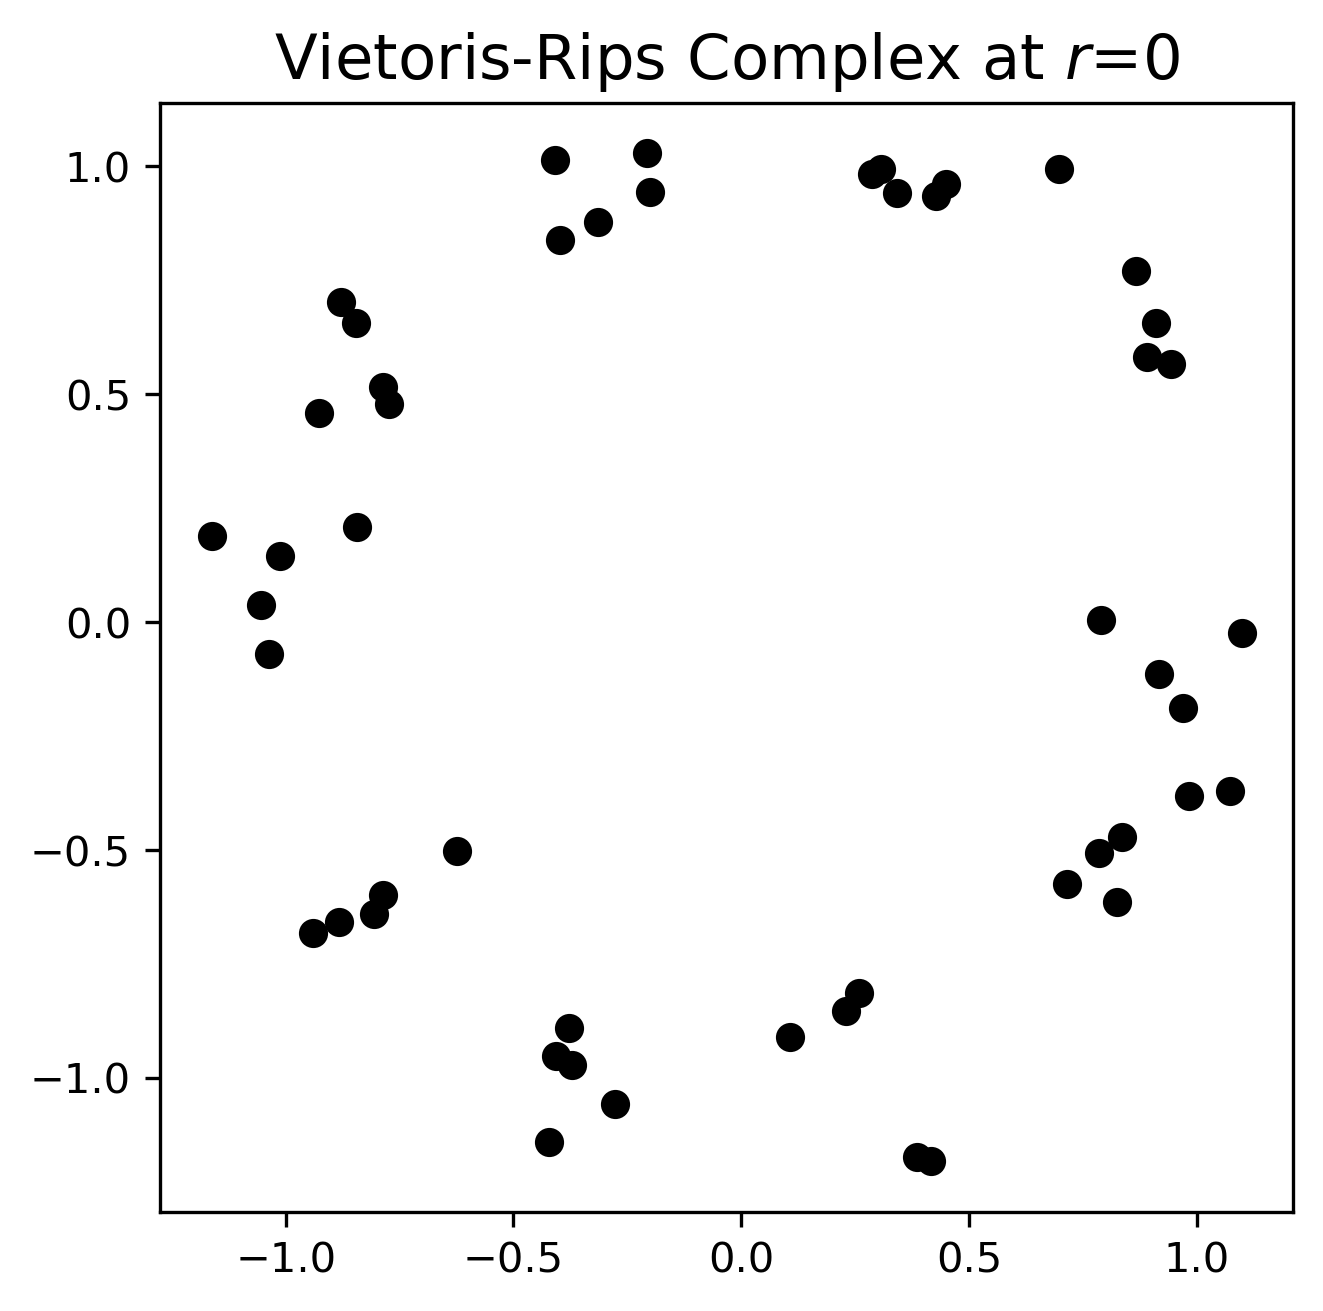
\includegraphics[width=\textwidth]{point_cloud_plot_r0.png}
    \end{subfigure}
    \hfill
    \begin{subfigure}[b]{0.22\textwidth}
        \centering
        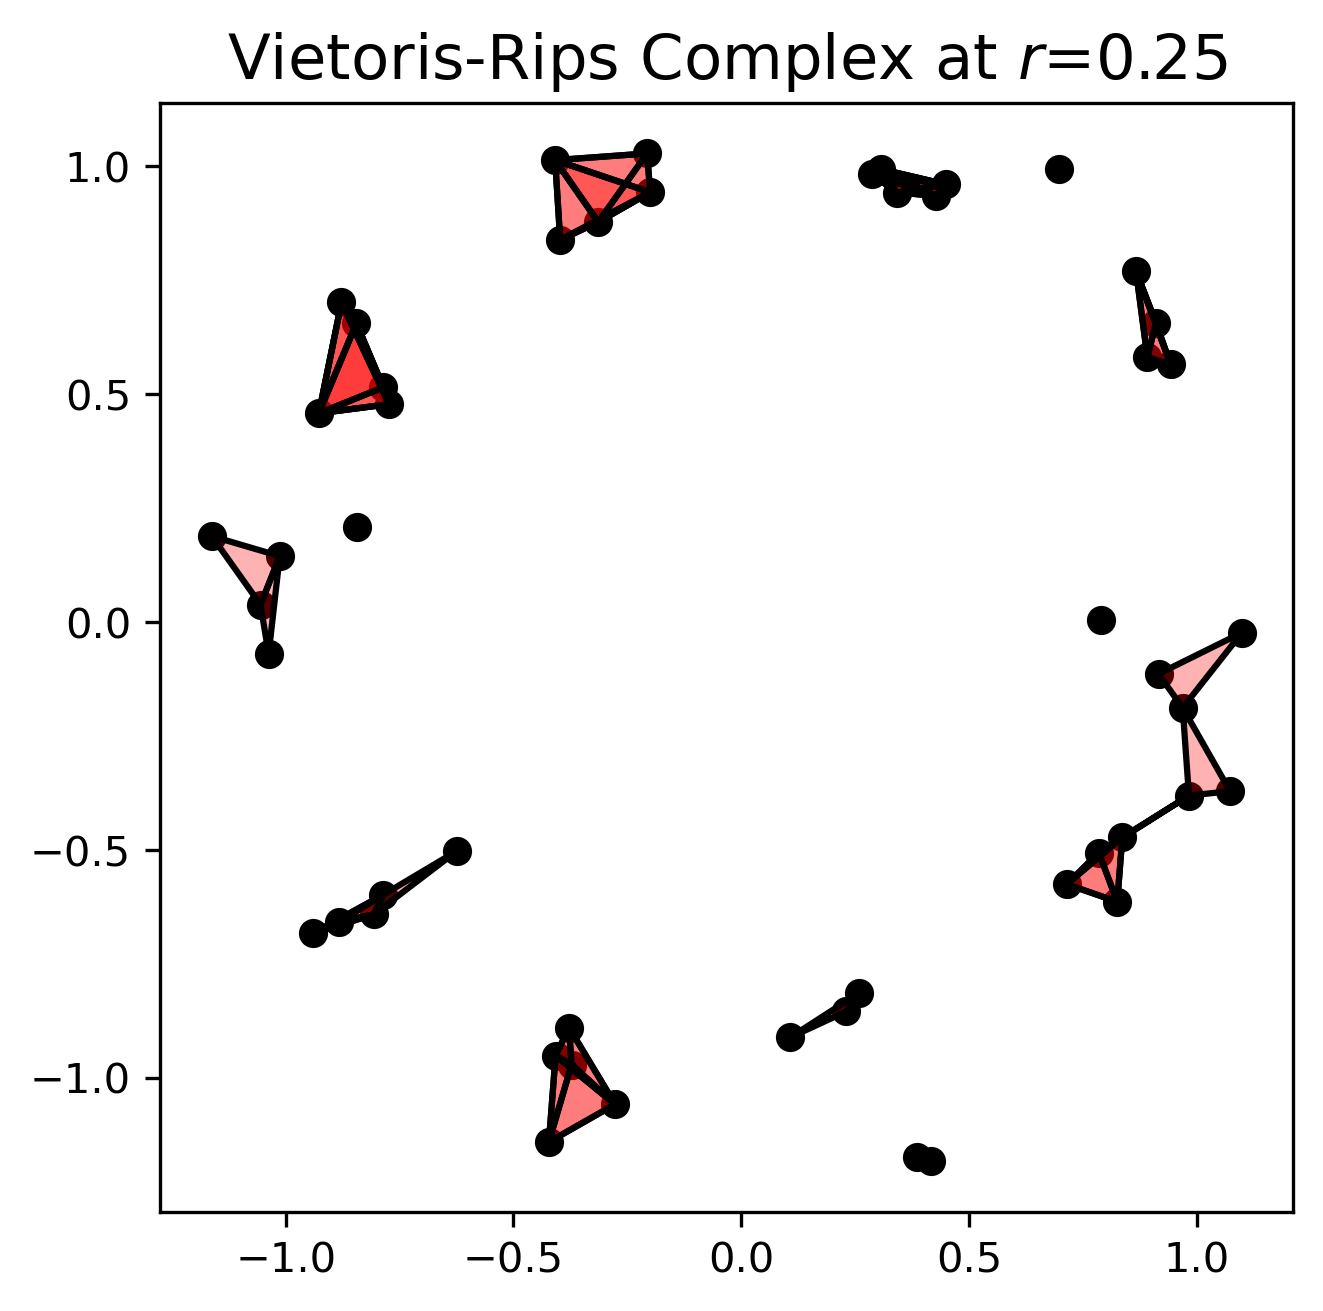
\includegraphics[width=\textwidth]{point_cloud_plot_r0_25.png}
    \end{subfigure}
        \hfill
    \begin{subfigure}[b]{0.22\textwidth}
        \centering
        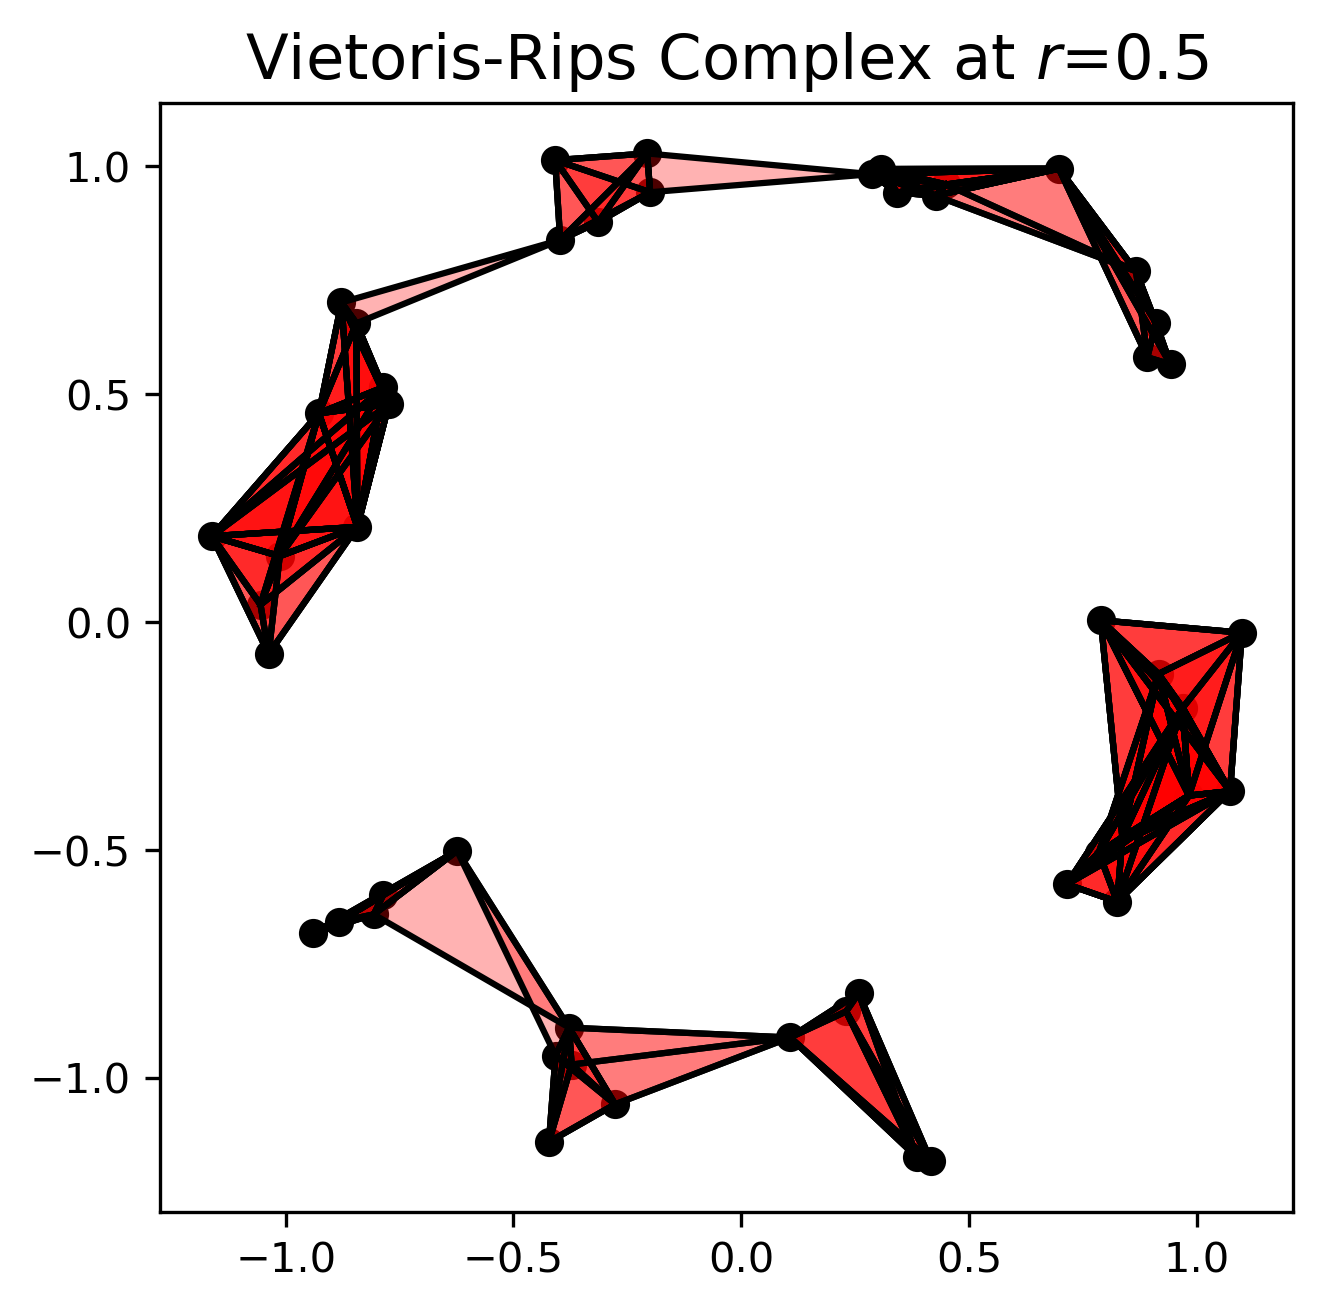
\includegraphics[width=\textwidth]{point_cloud_plot_r0_5.png}
    \end{subfigure}
        \hfill
    \begin{subfigure}[b]{0.22\textwidth}
        \centering
        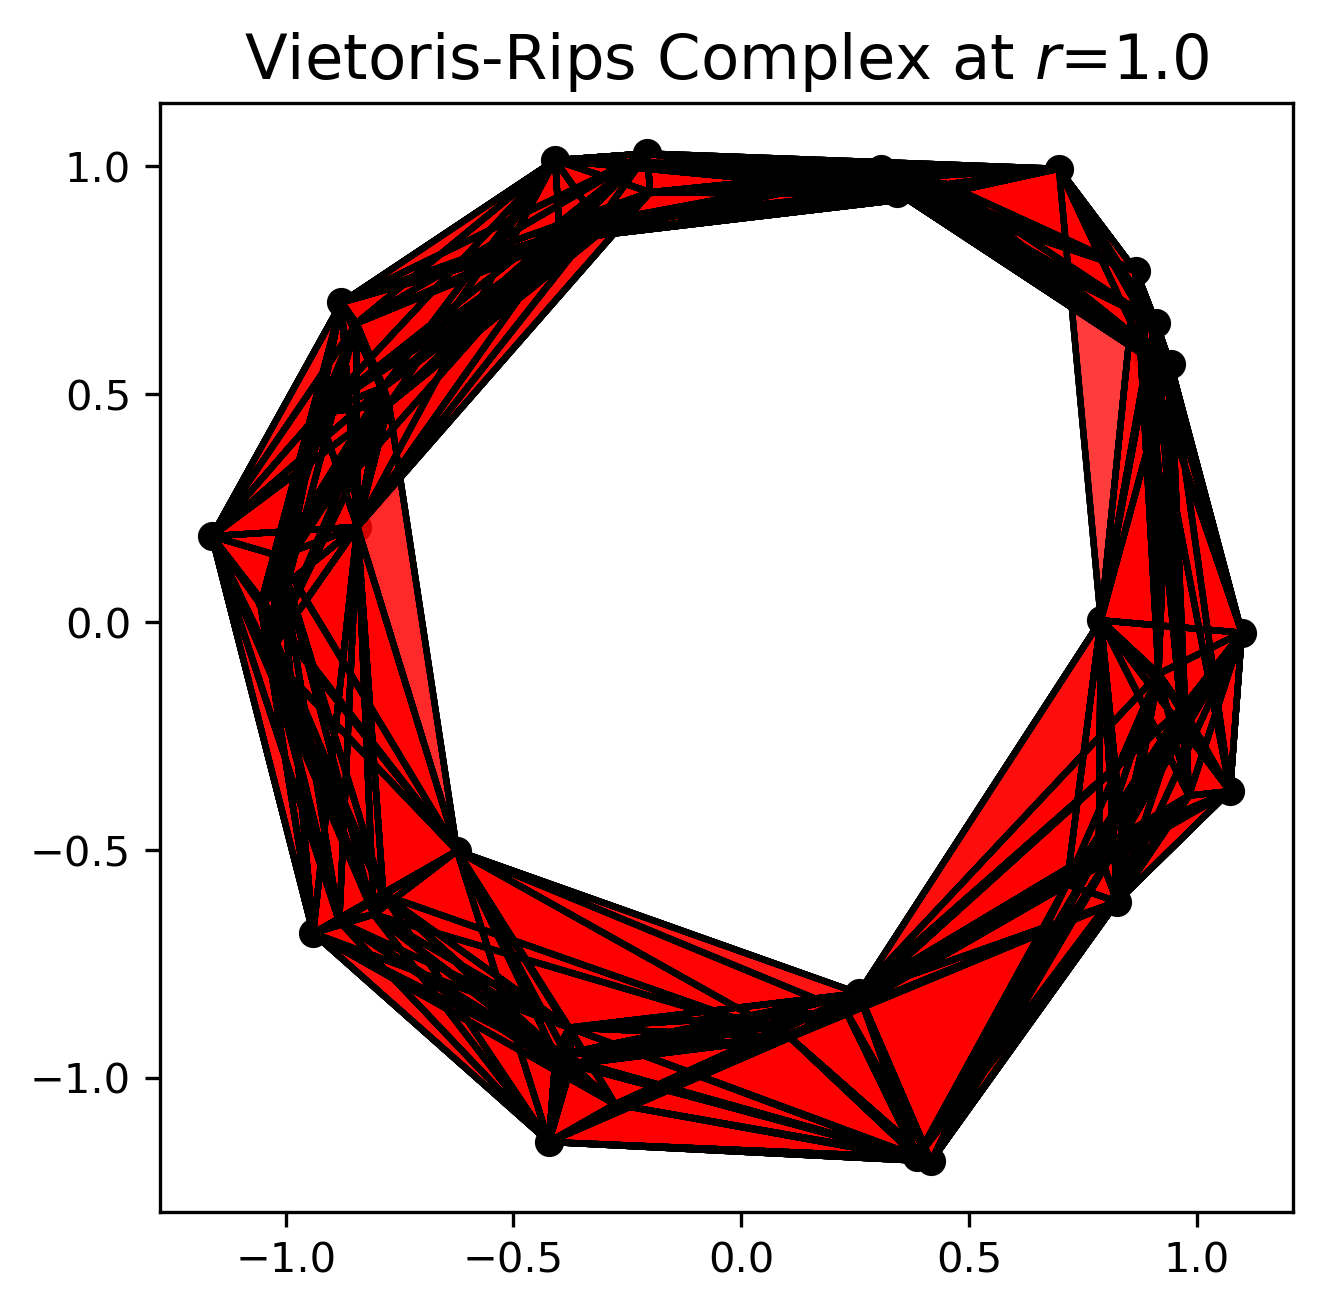
\includegraphics[width=\textwidth]{point_cloud_plot_r1_0.png}
    \end{subfigure}
    \caption{Vietoris-Rips complex of a point cloud as radius $r$ increases.}
    \label{fig:point_cloud_radii}
\end{figure}
\end{example}

\begin{example}[Persistence Diagram of a Vietoris-Rips Complex of a Point Cloud]
This example uses a randomly generated point cloud to create a persistence diagram from a Vietoris-Rips complex. When $r=0.5$, the persistence diagram shows three points at $d=\infty$ for $H_0$. This corresponds to the three connected components in the filtered simplicial complex. The points below infinity on the $y$-axis show the death times of points as they get added to one of the three connected components. Notice how there are only points on the $y$-axis: as Figure \ref{fig:point_cloud_radii} shows, all points are present when $r=0$, this means each point in the complex has a birth time of $0$.
\begin{figure}[H]
    \centering
    \begin{subfigure}[b]{0.45\textwidth}
        \centering
        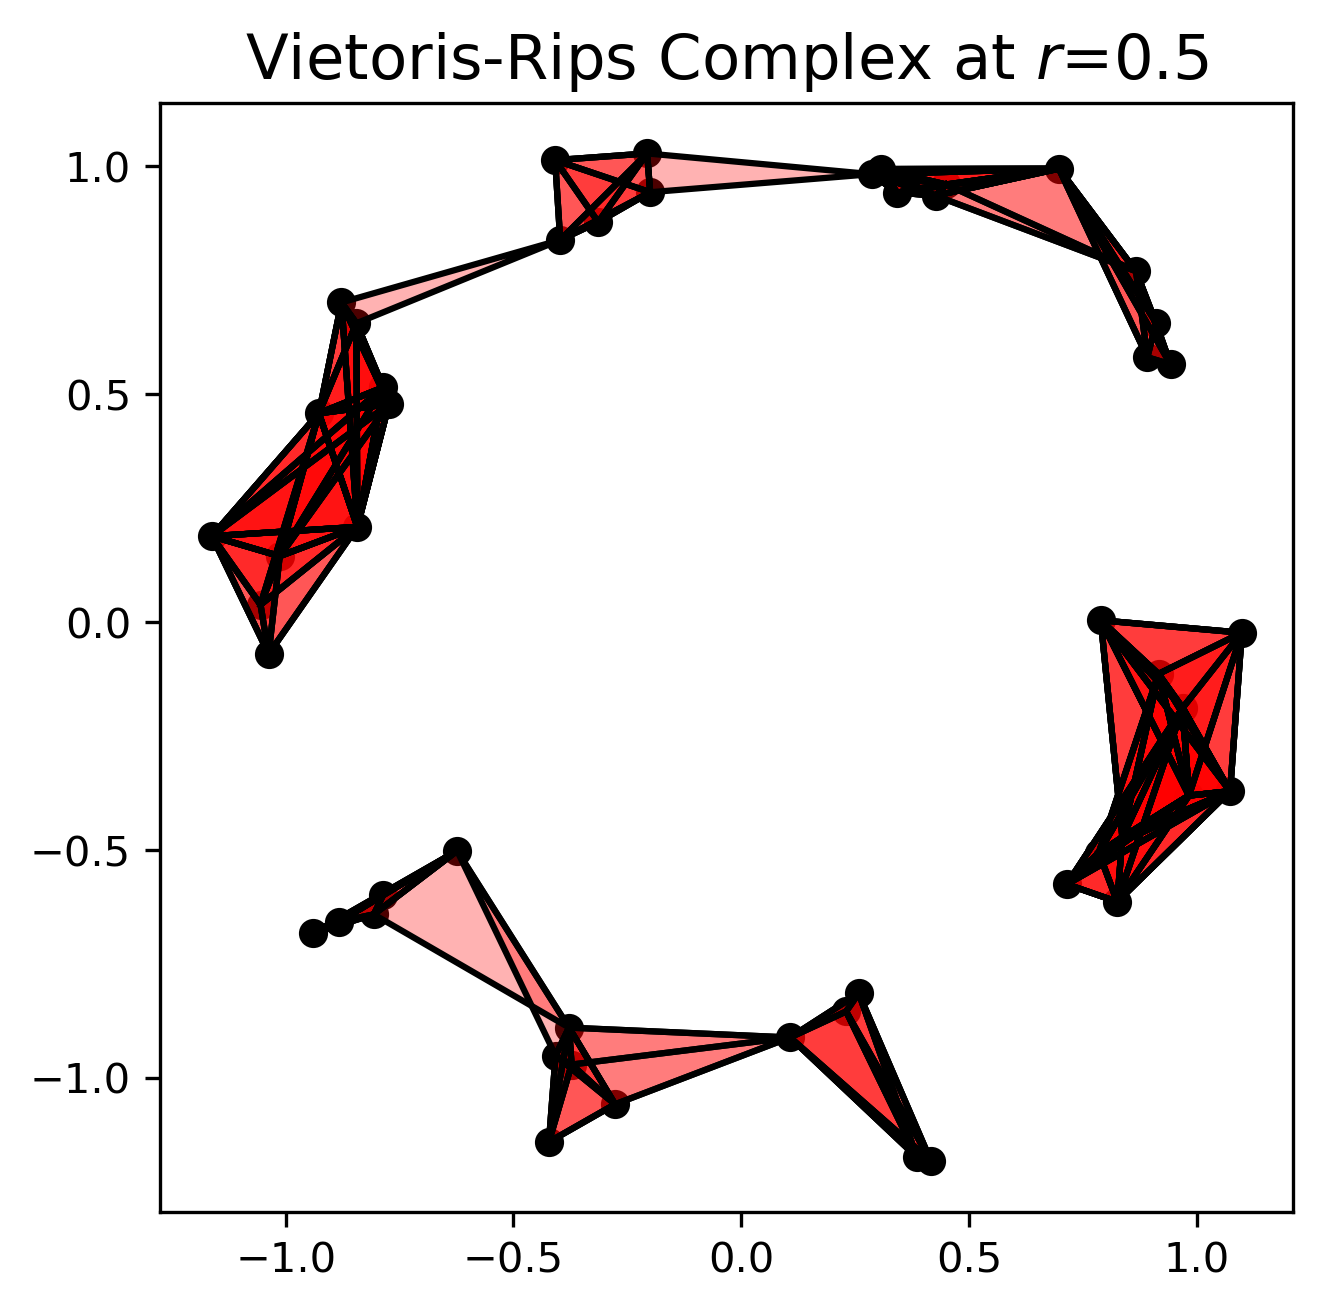
\includegraphics[width=\textwidth]{point_cloud_plot_r0_5.png}
    \end{subfigure}
    \hfill
    \begin{subfigure}[b]{0.45\textwidth}
        \centering
        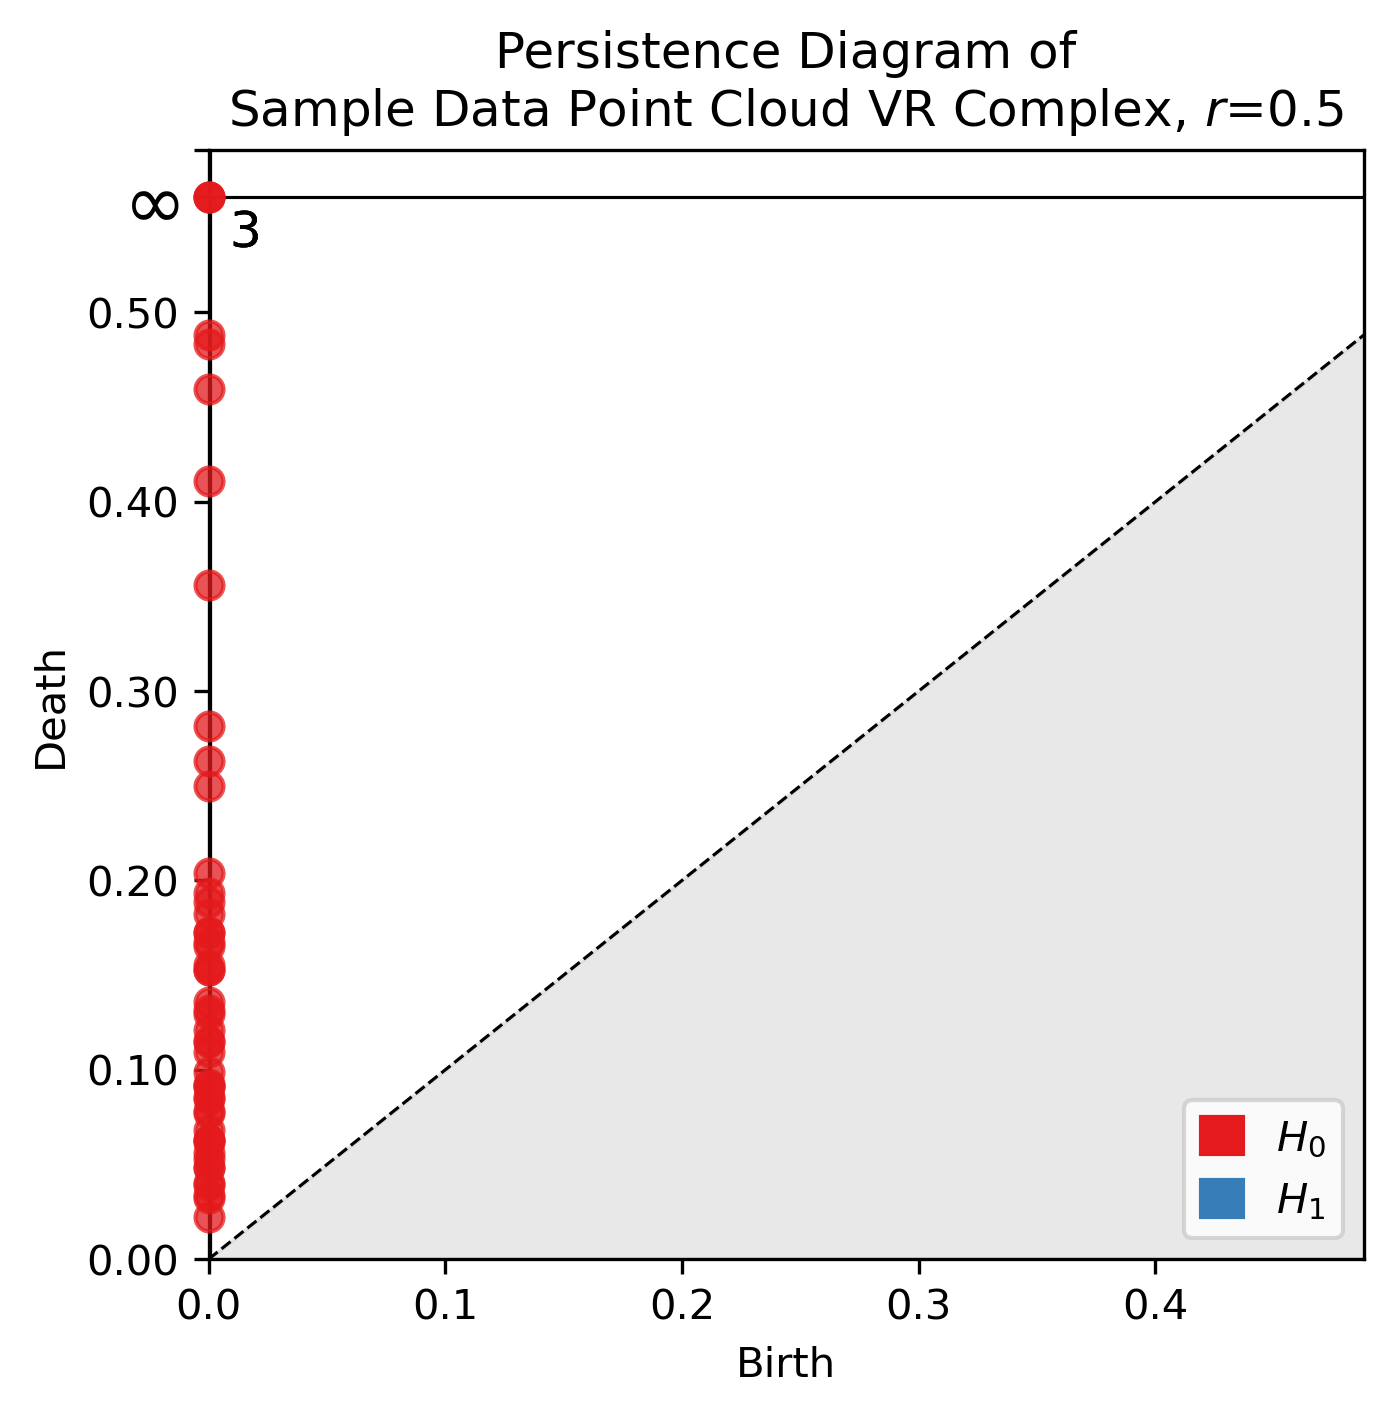
\includegraphics[width=\textwidth]{point_cloud_persdia_vr_0_5.png}
    \end{subfigure}
    \caption{Plot of a point cloud and persistence diagram of its Vietoris-Rips complex.}
    \label{fig:point_cloud_persdia}
\end{figure}
\end{example}

\newpage
\par The Čech and Vietoris-Rips complexes can be very computationally expensive, so an alternative filtered simplicial complex, the Alpha Complex, will need to be applied to the STL file data. Before we can define the Alpha Complex, we need to define an essential component of it, the Delaunay Triangulation.


\begin{definition}[Delaunay Triangulation] A \textit{Delaunay triangulation} on a vector space is the dual of its Voronoi cells (Def \ref{def:voronoi}). The triangulation is created by creating a connection between points whenever their voronoi cells intersect \cite{deltri}.
\end{definition}
\begin{figure}[H]
    \centering
    \begin{subfigure}[b]{0.45\textwidth}
        \centering
        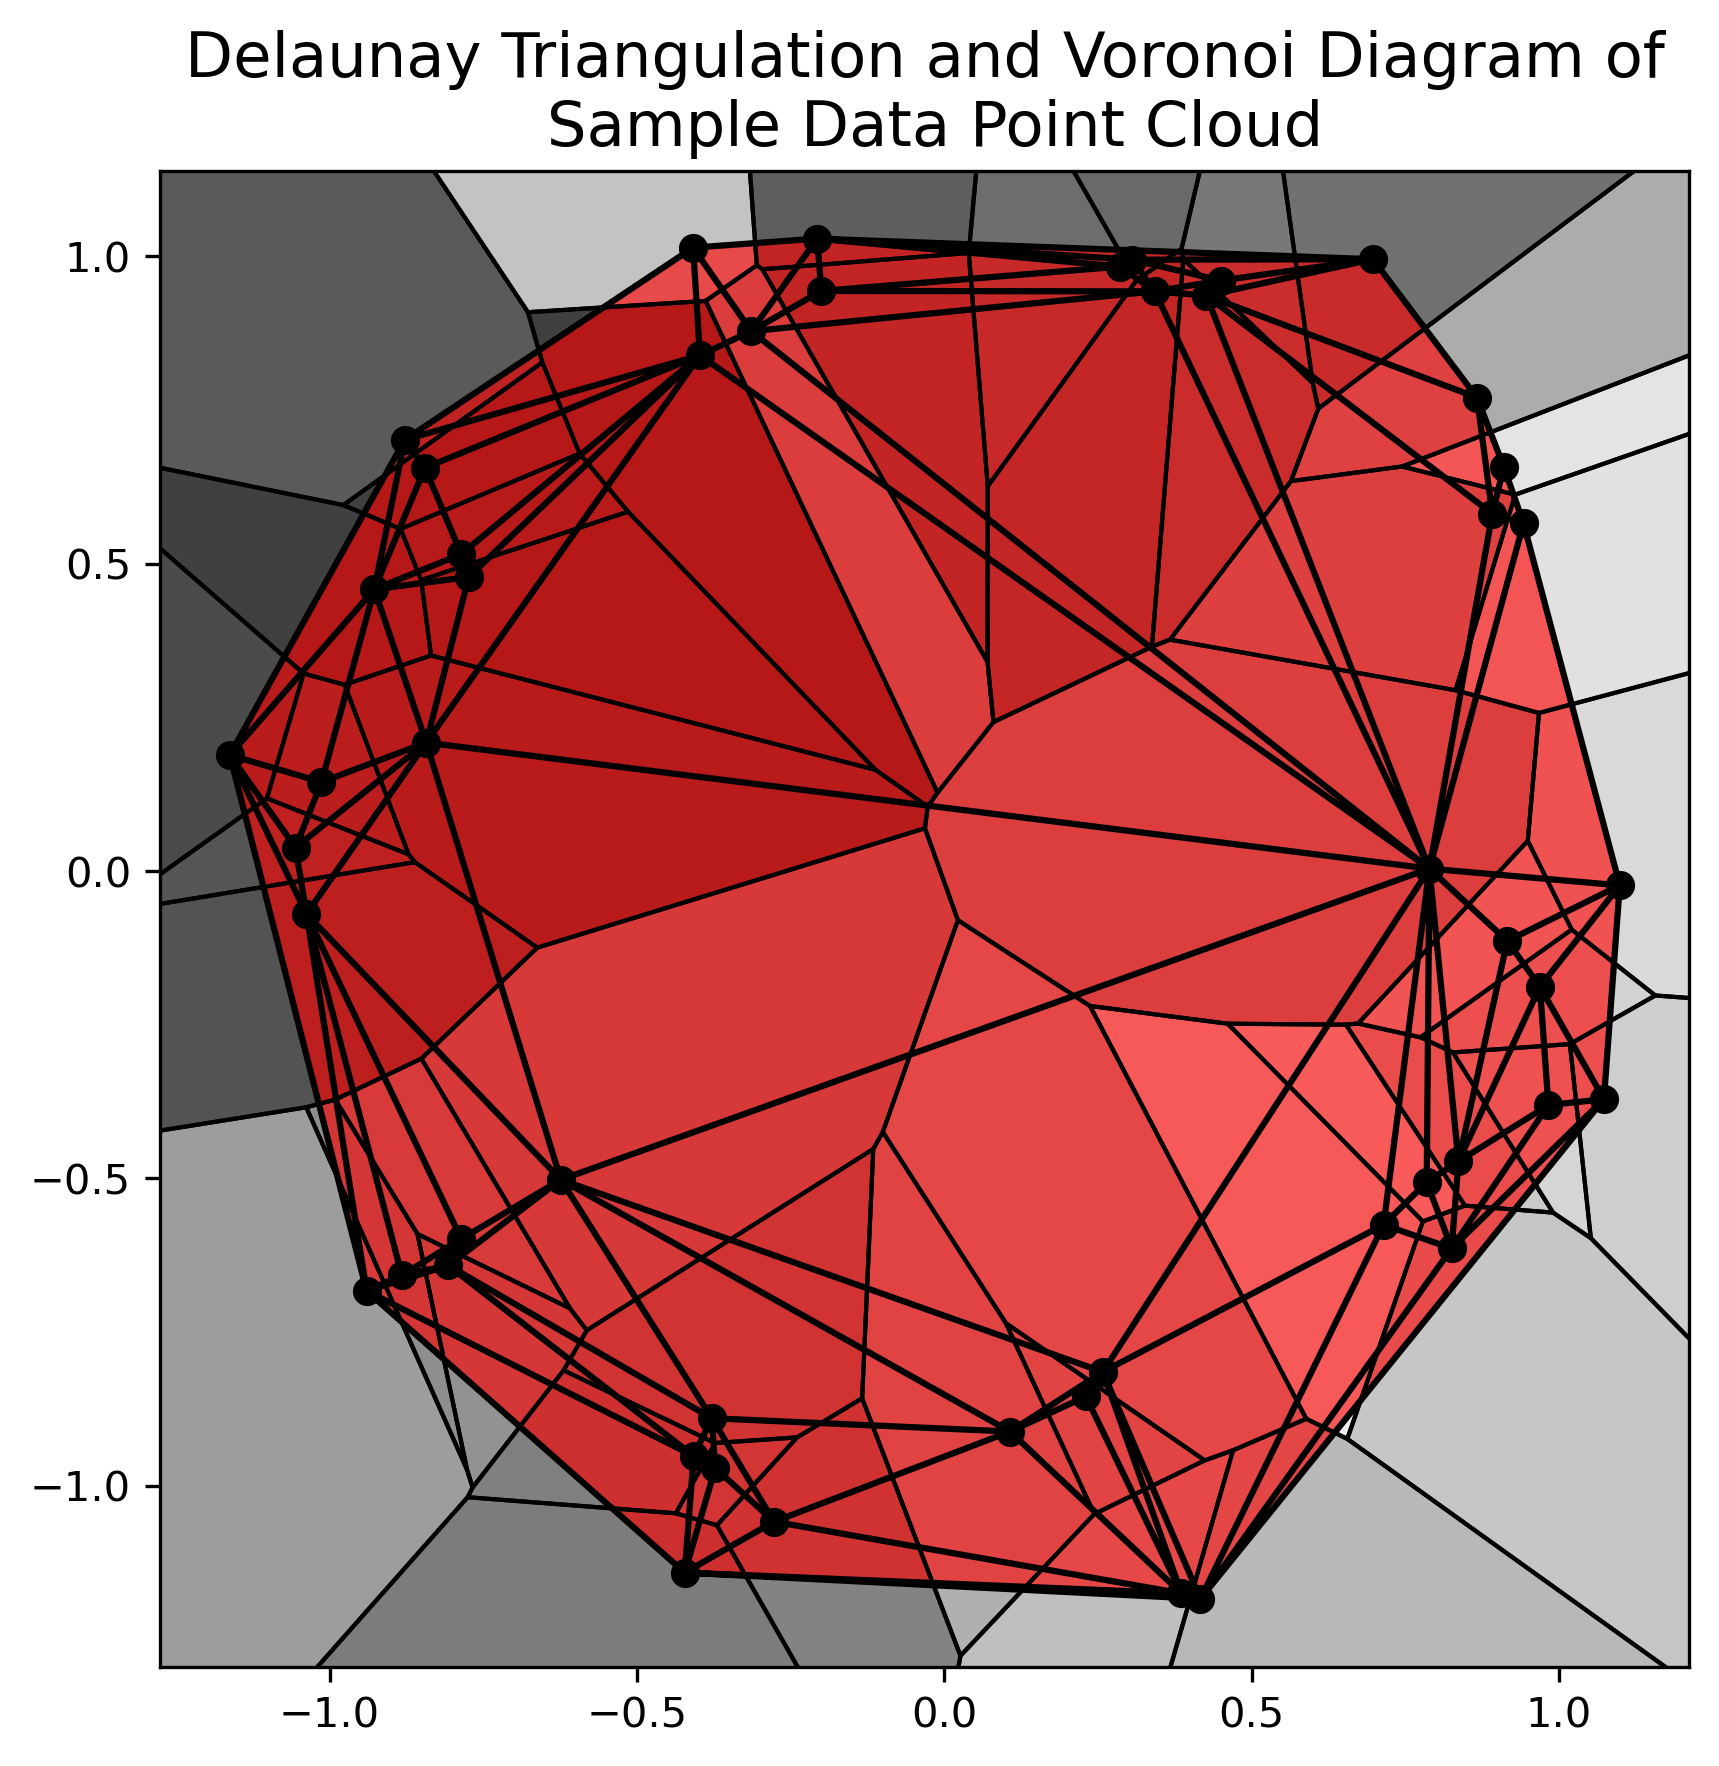
\includegraphics[width=\textwidth]{point_cloud_plot_del.png}
    \end{subfigure}
    \caption{Plot of a Delaunay Complex and Voronoi Cells applied to a point cloud.}
    \label{fig:point_cloud_del_persdia}
\end{figure}

\begin{definition}[Alpha Complexes]
The Alpha complex (or $\alpha$-complex) exists within a finite metric space $(X, d)$ which is isometrically embedded in $\mathbb{R}^{m}$ (or another larger metric space, $(Y, d)$) with Euclidean distance. The alpha complex builds upon the Delaunay Triangulation with its use of Voronoi cells by introducing a radius parameter for an open metric ball. 
$$\alpha_{r}(X)=\{\sigma \subseteq X \mid \cap_{x\in \sigma} (B_{r}(X) \cap \mathsf{Vor}_{x}) \not= \emptyset\}$$
At $r=0$, the filtered simplicial complex consists only of the set of points in the metric space as individual connected components. As $r$ increases, the balls grow up to the boundary of or beyond their Voronoi cell. When two balls intersect, a connected component between those two points is formed. This continues until $r$ grows to create a simplex equivalent to the Delaunay triangulation.
\end{definition}

\newpage
\begin{example}[Alpha Complex applied to a Point Cloud]\label{ex:point_cloud_alpha}
\par This example shows an Alpha complex created with the python library \verb"gudhi", which defines its growing radii parameter as $r^{2}$ to birth and death times. To understand events at certain radii, we denote plots with $r^{2}$ for birth and death times, and $r$ for Euclidean distance.
\par Two holes were created with birth times of $r^{2}=0.2308$ and $r^{2}=0.3068$. The first hole dies at $r^{2}=0.8045$, while the second hole dies relatively quickly at $r^{2}=0.3069$. The second hole dies so quickly because . The hole then dies and is formed $r^{2}=0.0001$ later because .
\begin{figure}[H]
    \centering
    \begin{subfigure}[b]{0.28\textwidth}
        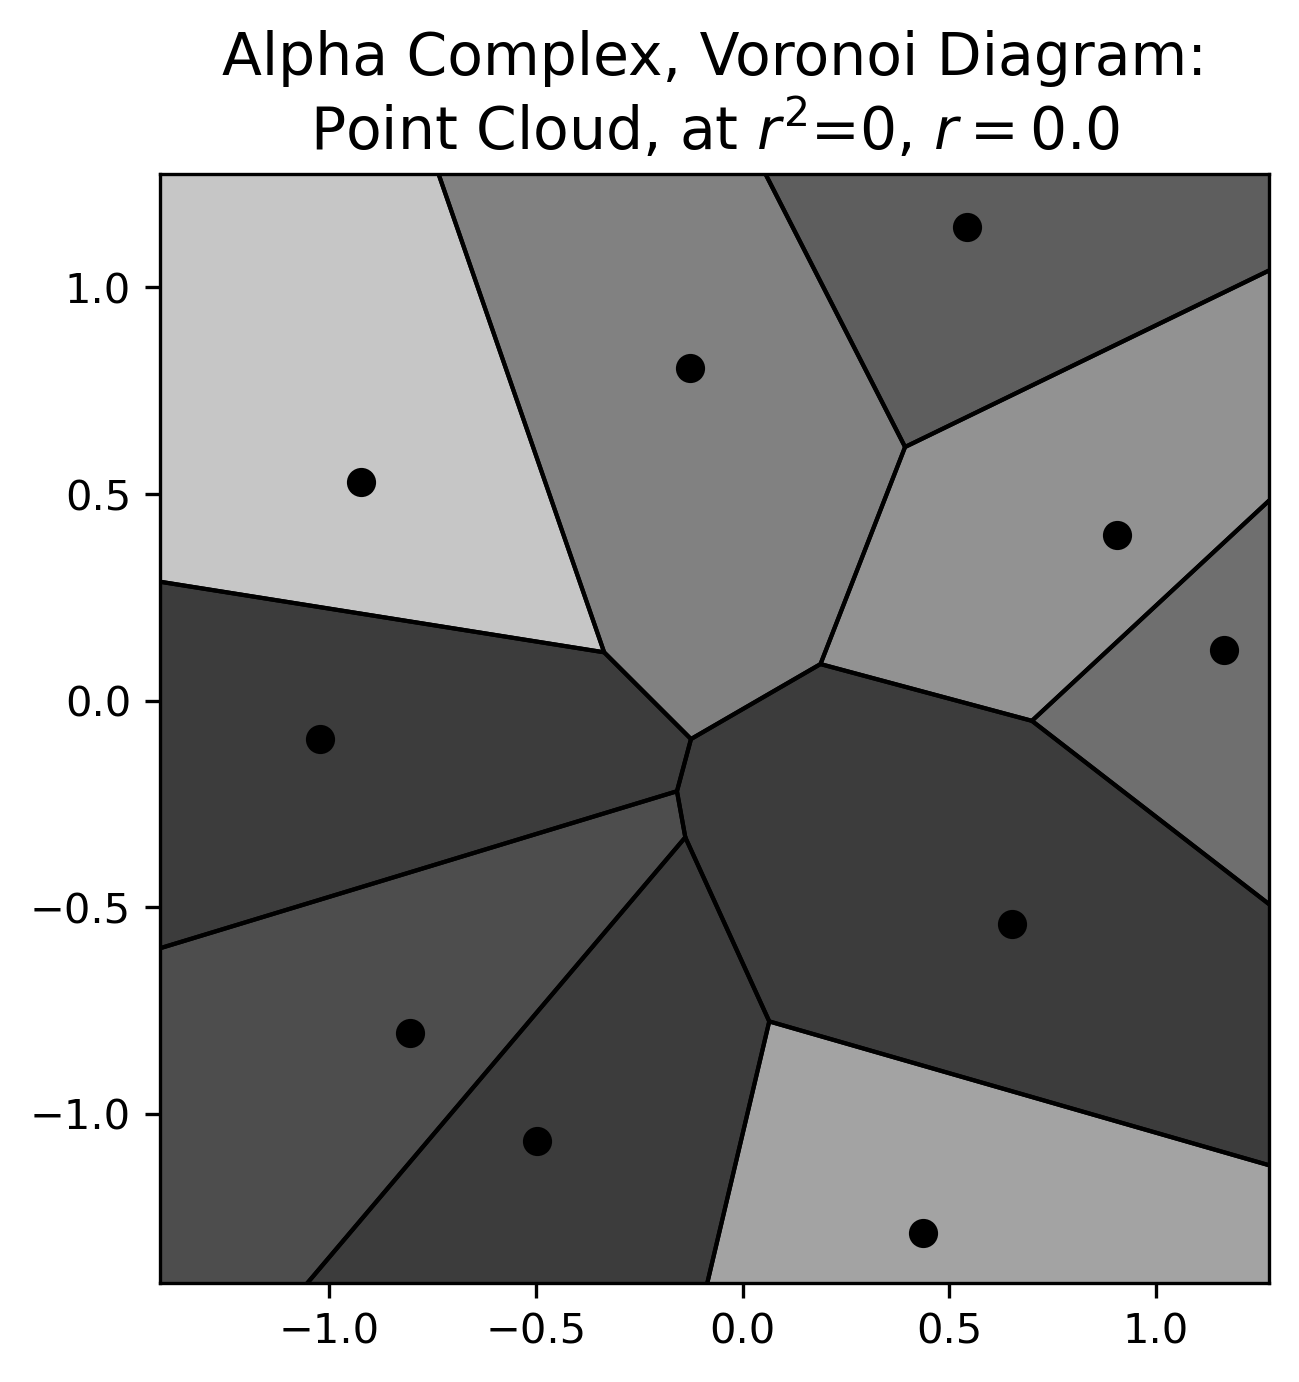
\includegraphics[width=\textwidth]{point_cloud_plot_alpha_0.png}
    \end{subfigure}
    \hfill
    \begin{subfigure}[b]{0.28\textwidth}
        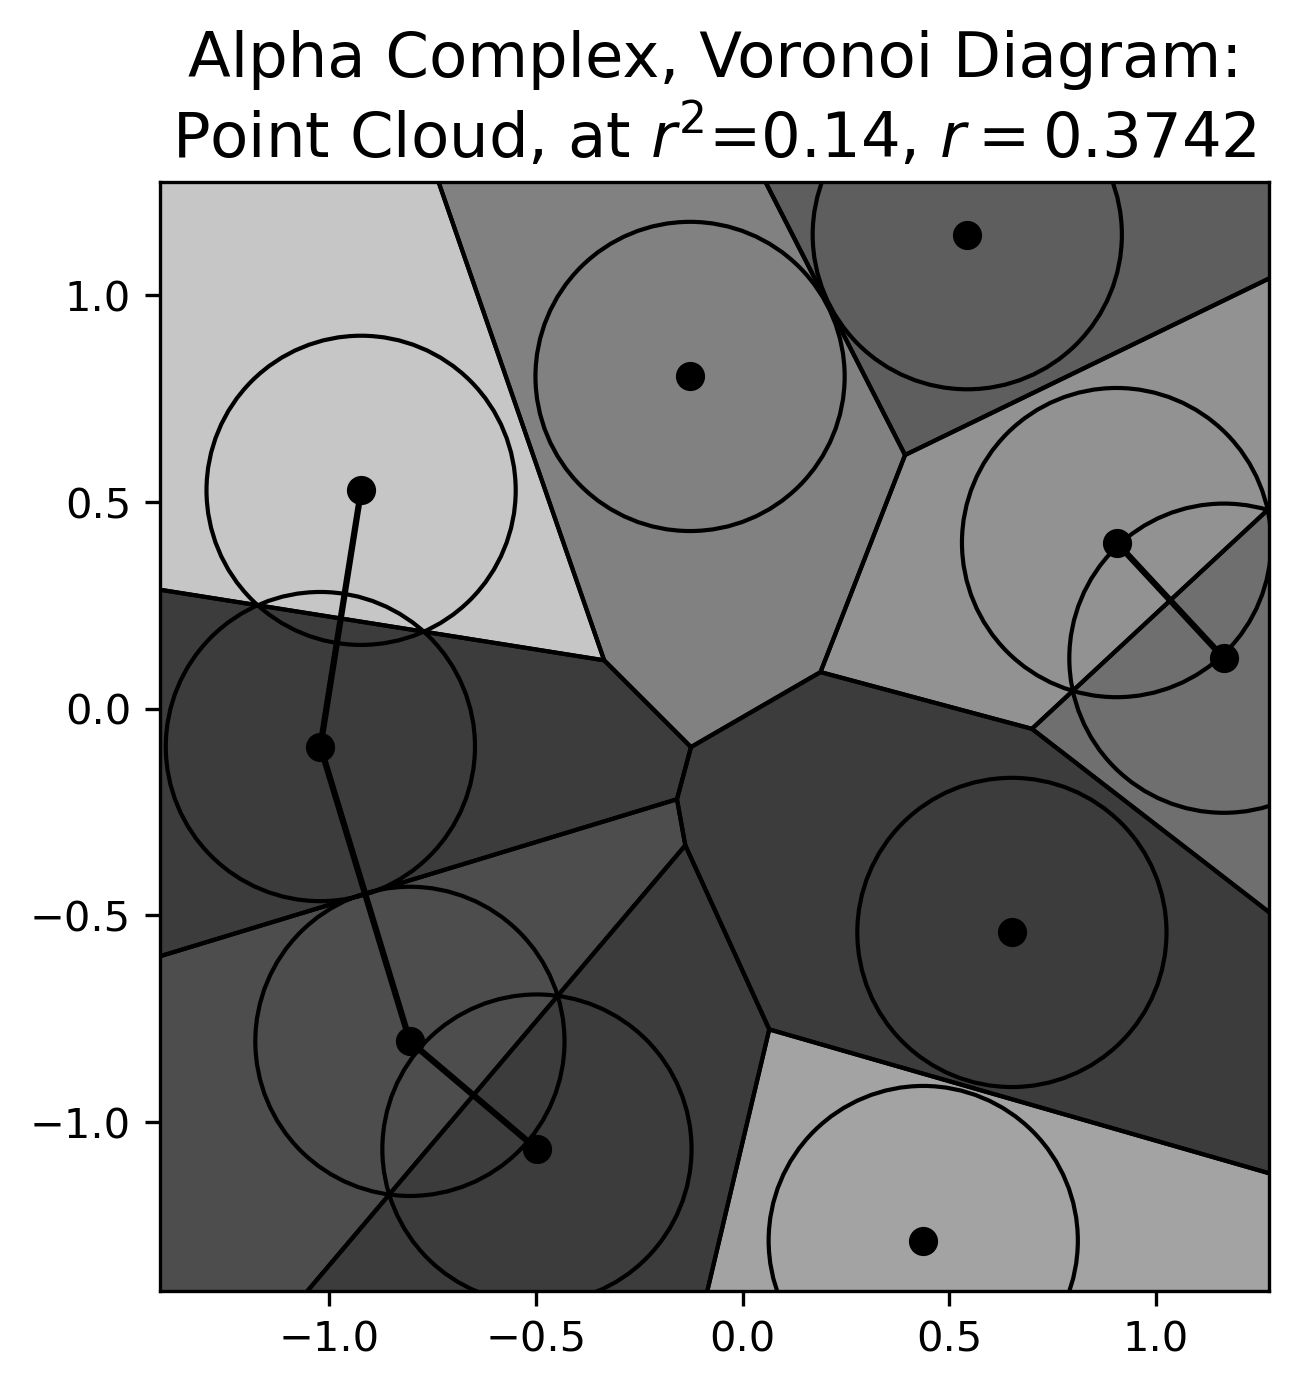
\includegraphics[width=\textwidth]{point_cloud_plot_alpha_1.png}
    \end{subfigure}
    \hfill
    \begin{subfigure}[b]{0.28\textwidth}
        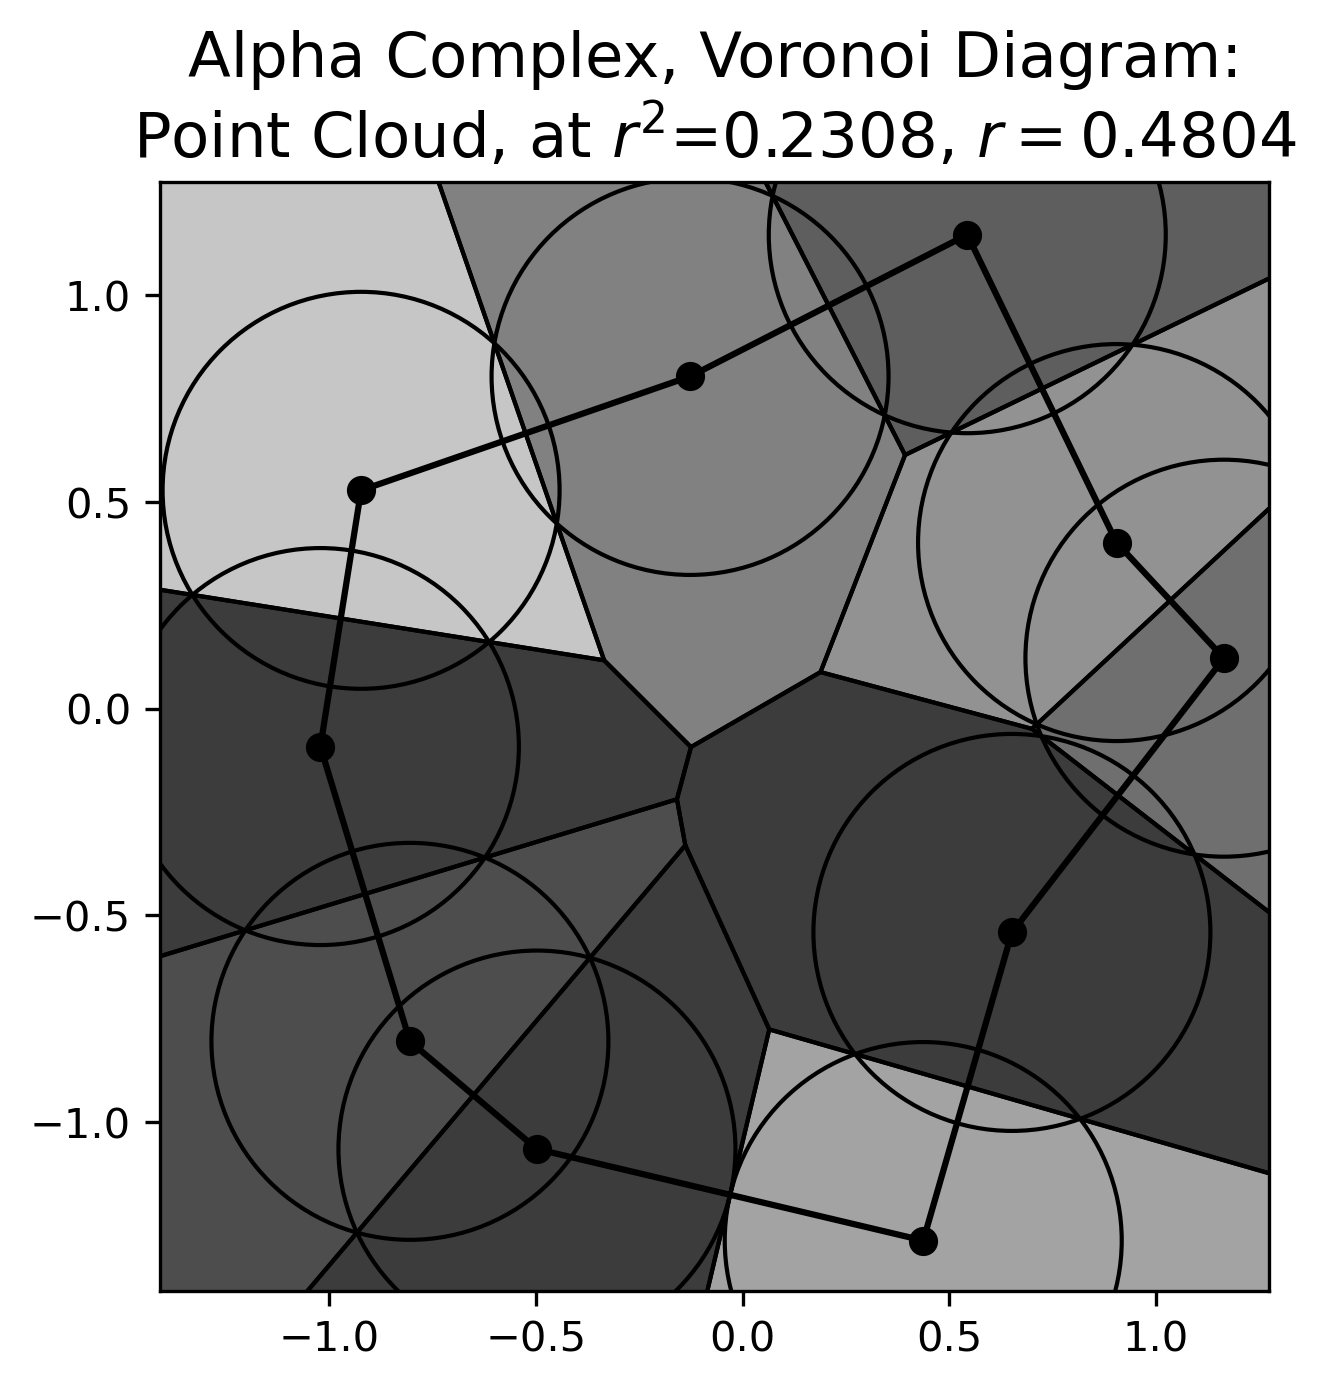
\includegraphics[width=\textwidth]{point_cloud_plot_alpha_2.png}
    \end{subfigure}
    \hfill
    \begin{subfigure}[b]{0.28\textwidth}
        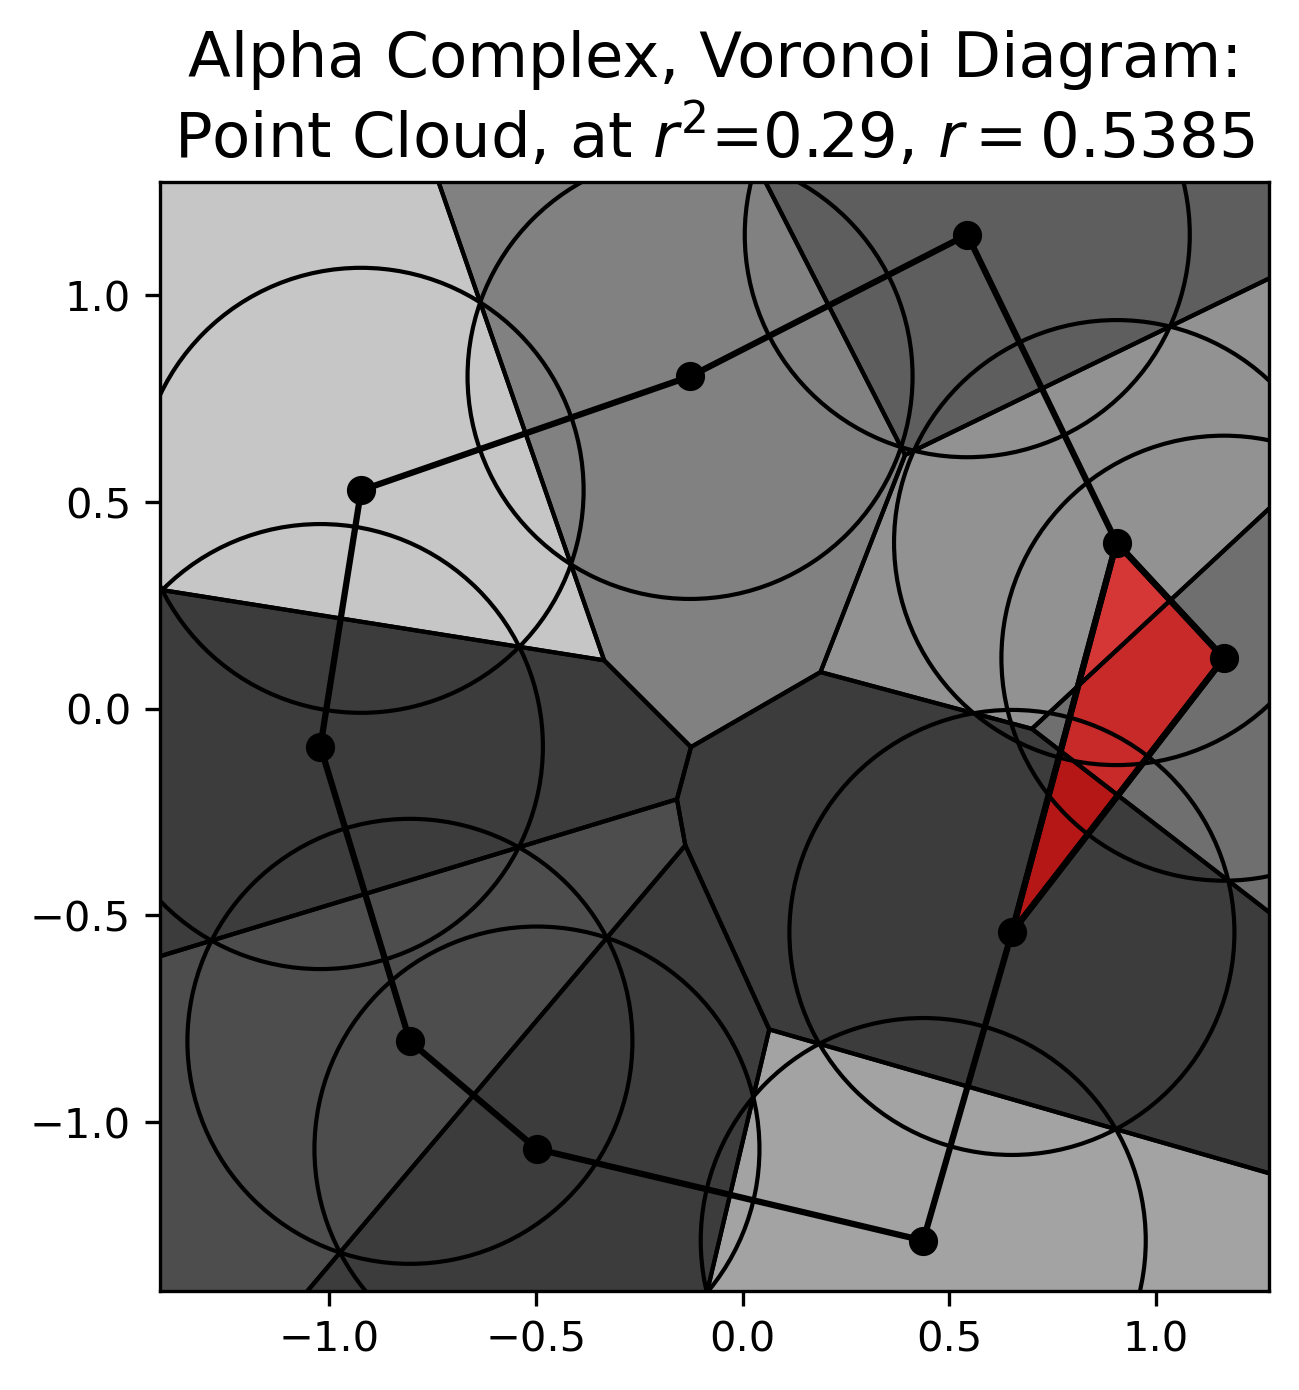
\includegraphics[width=\textwidth]{point_cloud_plot_alpha_3.png}
    \end{subfigure}
    \hfill
    \begin{subfigure}[b]{0.28\textwidth}
        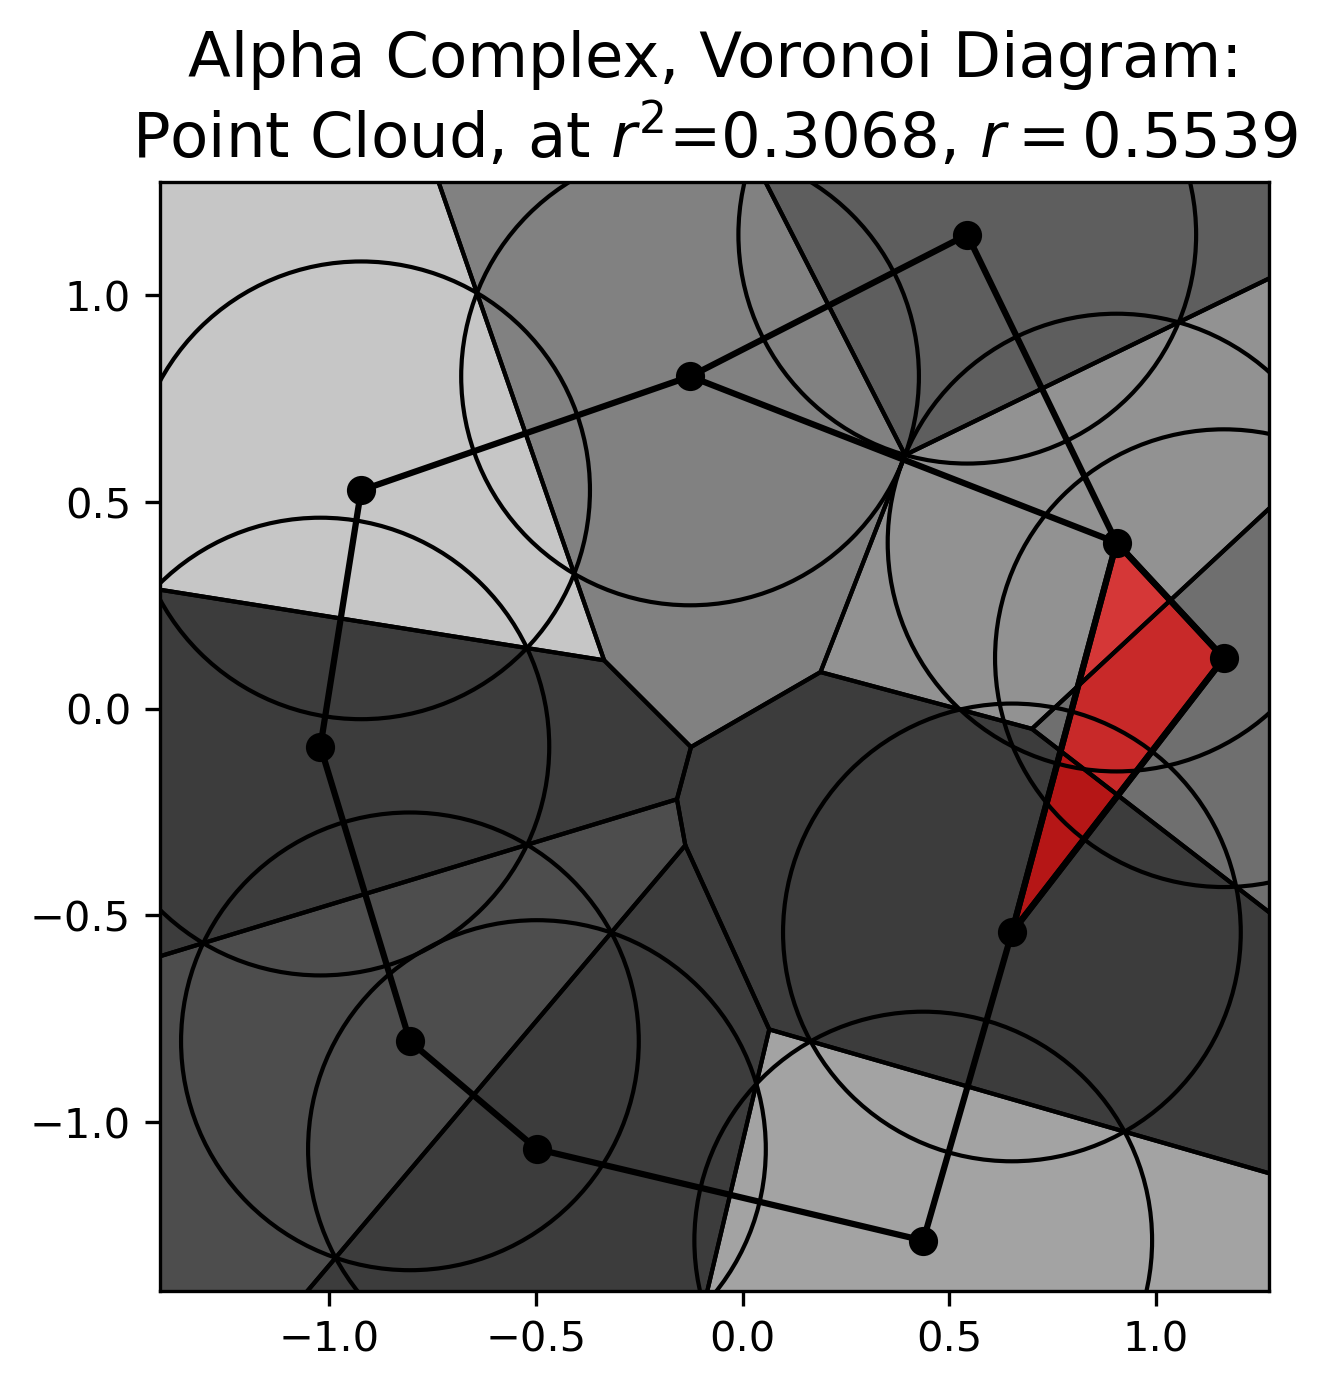
\includegraphics[width=\textwidth]{point_cloud_plot_alpha_4.png}
    \end{subfigure}
    \hfill
    \begin{subfigure}[b]{0.28\textwidth}
        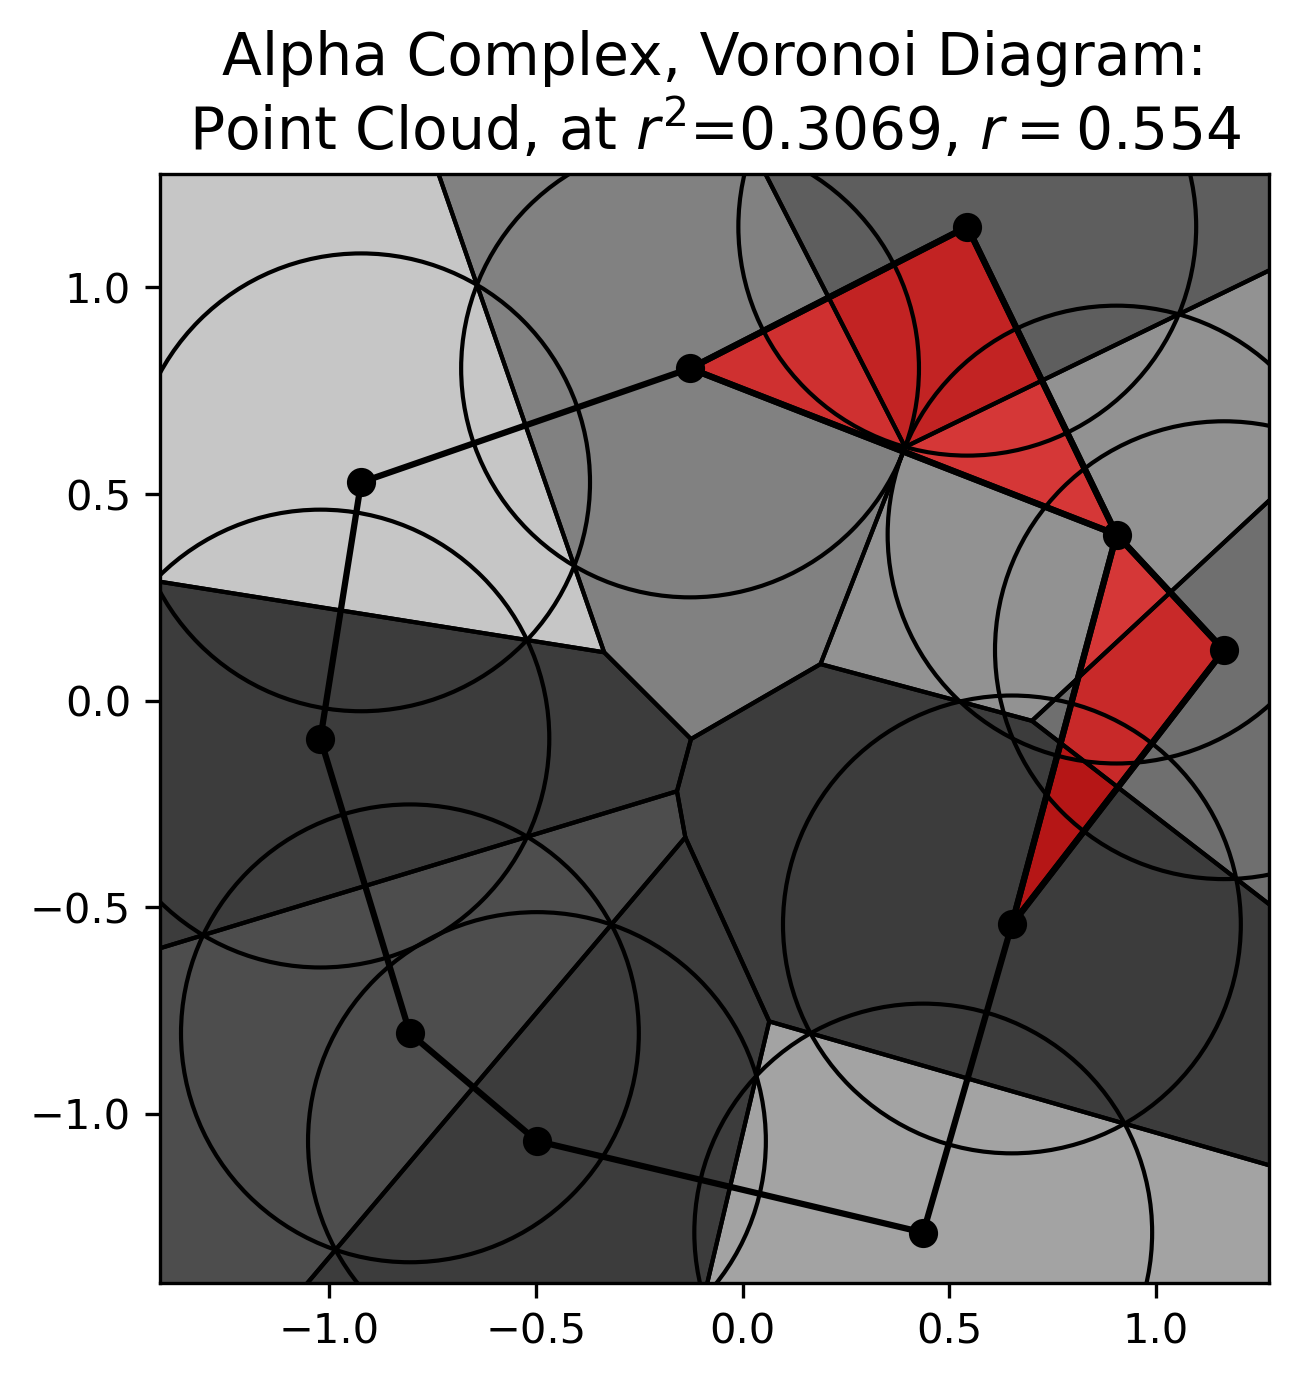
\includegraphics[width=\textwidth]{point_cloud_plot_alpha_5.png}
    \end{subfigure}
    \hfill
    \begin{subfigure}[b]{0.28\textwidth}
        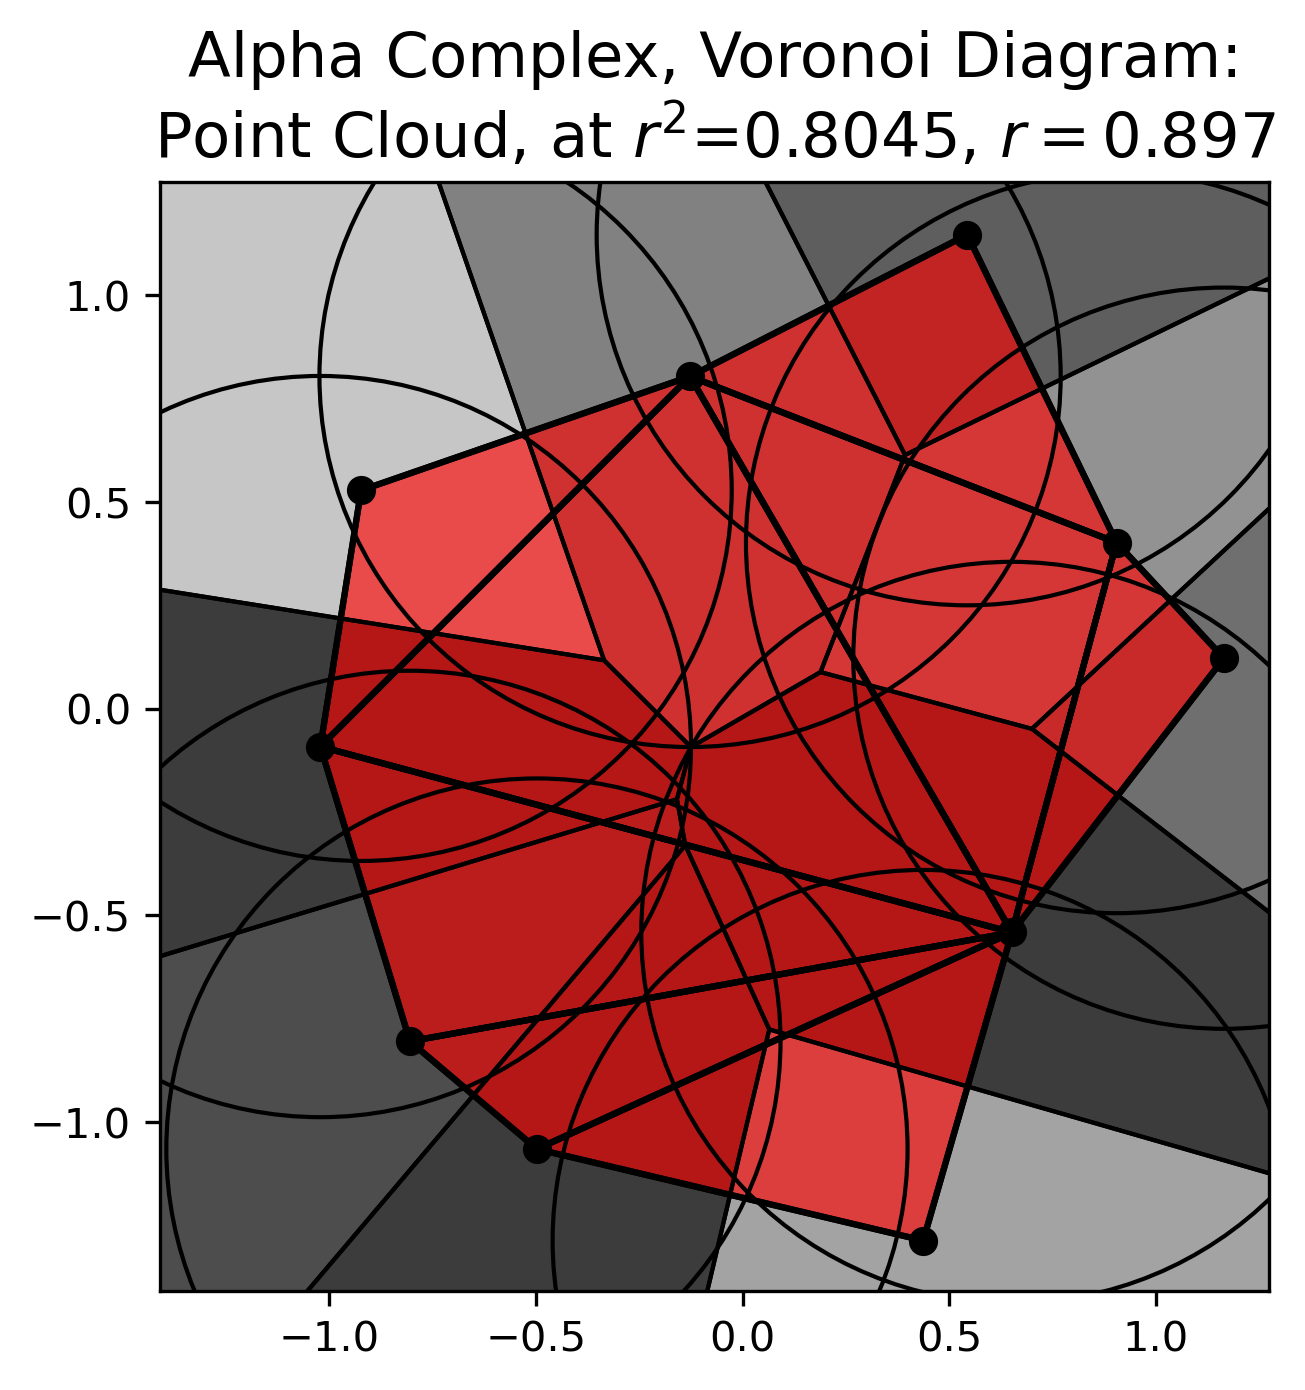
\includegraphics[width=\textwidth]{point_cloud_plot_alpha_6.png}
    \end{subfigure}
    \hfill
    \begin{subfigure}[b]{0.28\textwidth}
        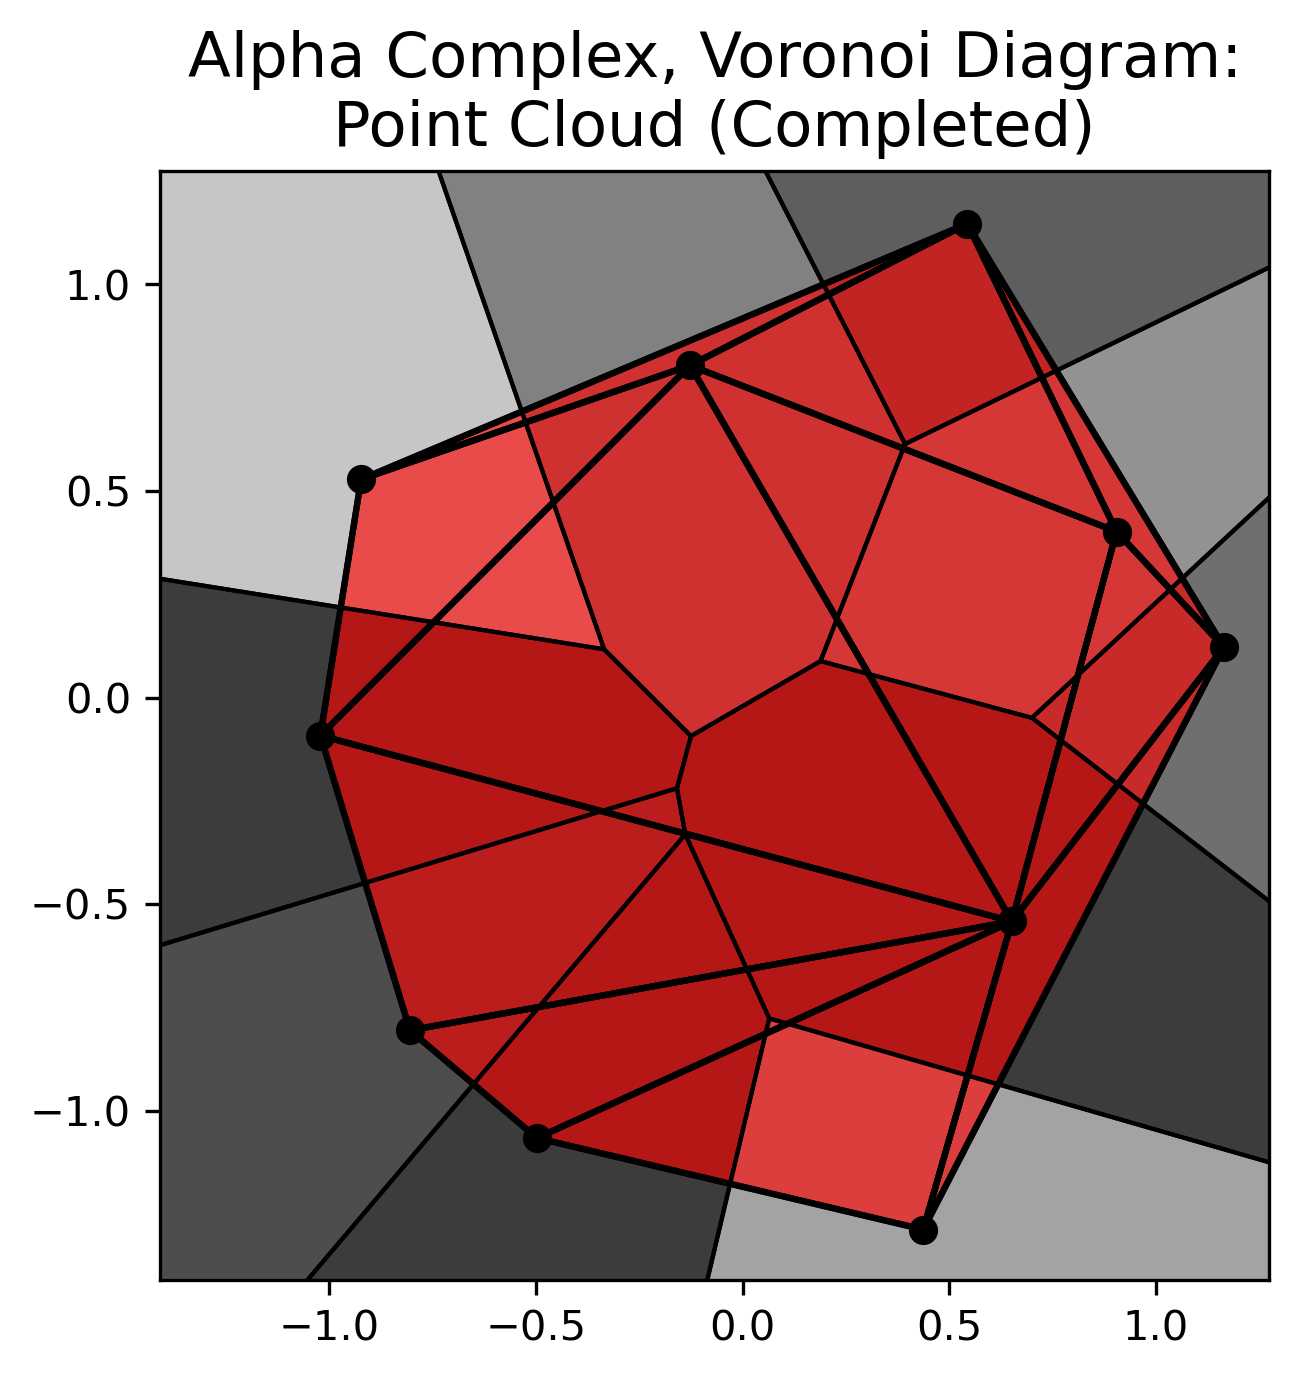
\includegraphics[width=\textwidth]{point_cloud_plot_alpha_voronoi.png}
    \end{subfigure}
    \hfill
    \begin{subfigure}[b]{0.28\textwidth}
        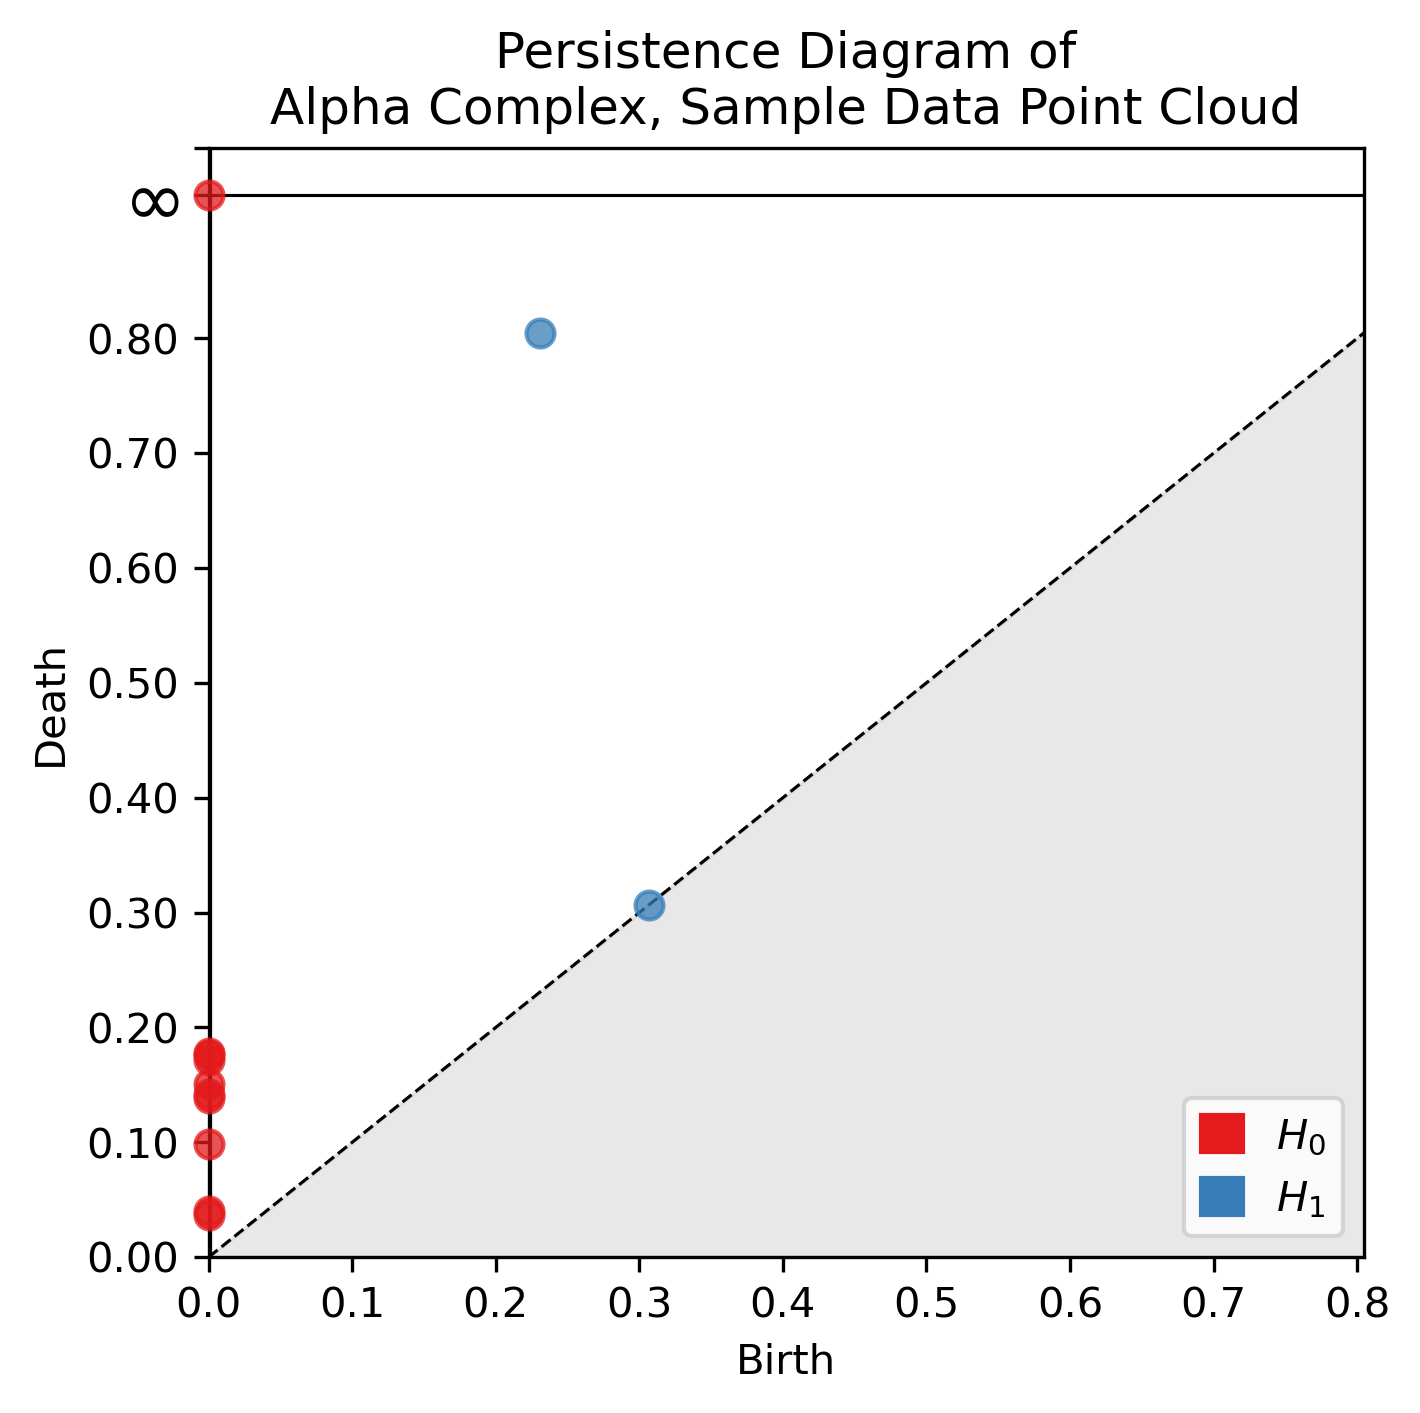
\includegraphics[width=\textwidth]{point_cloud_persdia_alpha_voronoi.png}
    \end{subfigure}

    \caption{Progression of the Alpha complex on a point cloud and the persistence diagram of the completed complex.}
    \label{fig:point_cloud_alpha_complex}
\end{figure}
\end{example}

\newpage
\begin{example}[Persistence Diagram of an Image]
This example uses a grayscale image of a white square with a black circle in the center to create a persistence diagram from an Alpha complex. Although the image seems like a bullet point in a blank area, thanks to the nature of the grayscale data, the white pixels in the image contain values of 1 and the black pixels contain no data, or values of 0. In other words, the black circle is a hole in the data which can be seen as a point in $H_1$ with a birth time of 0. On a persistence diagram, the points along or relatively close to the diagonal line which are not on the $y$-axis can be considered noise and disregarded.
\begin{figure}[H]
    \centering
    \begin{subfigure}[b]{0.45\textwidth}
        \centering
        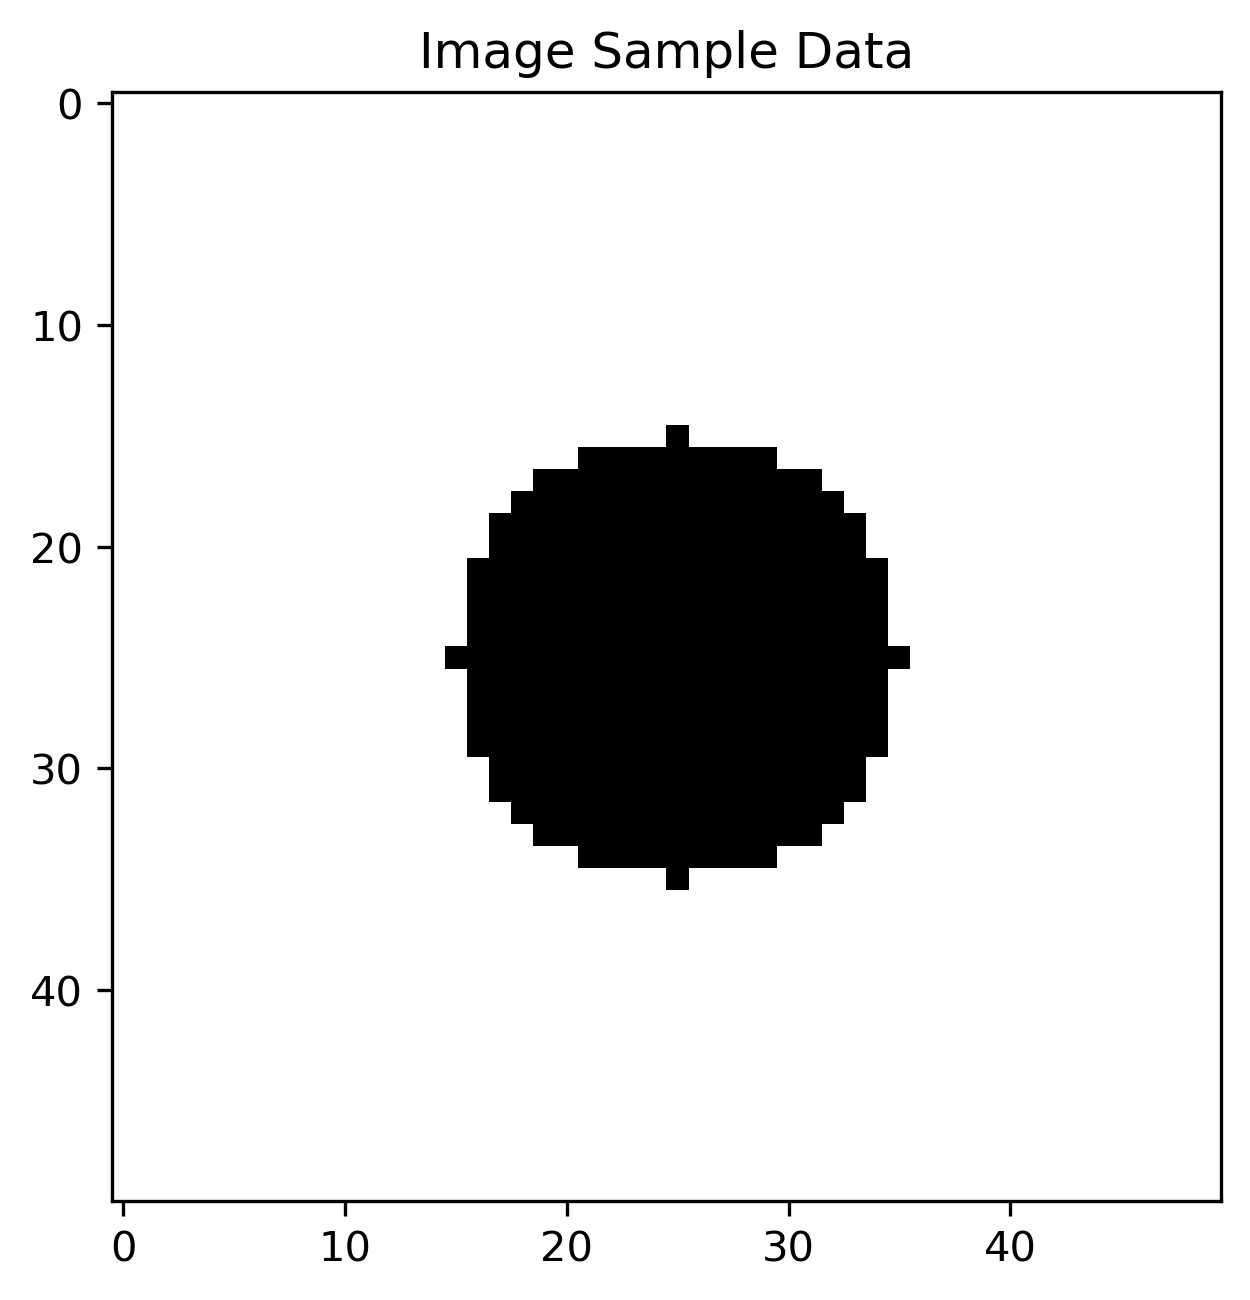
\includegraphics[width=\textwidth]{image_data_plot.png}
    \end{subfigure}
    \hfill
    \begin{subfigure}[b]{0.45\textwidth}
        \centering
        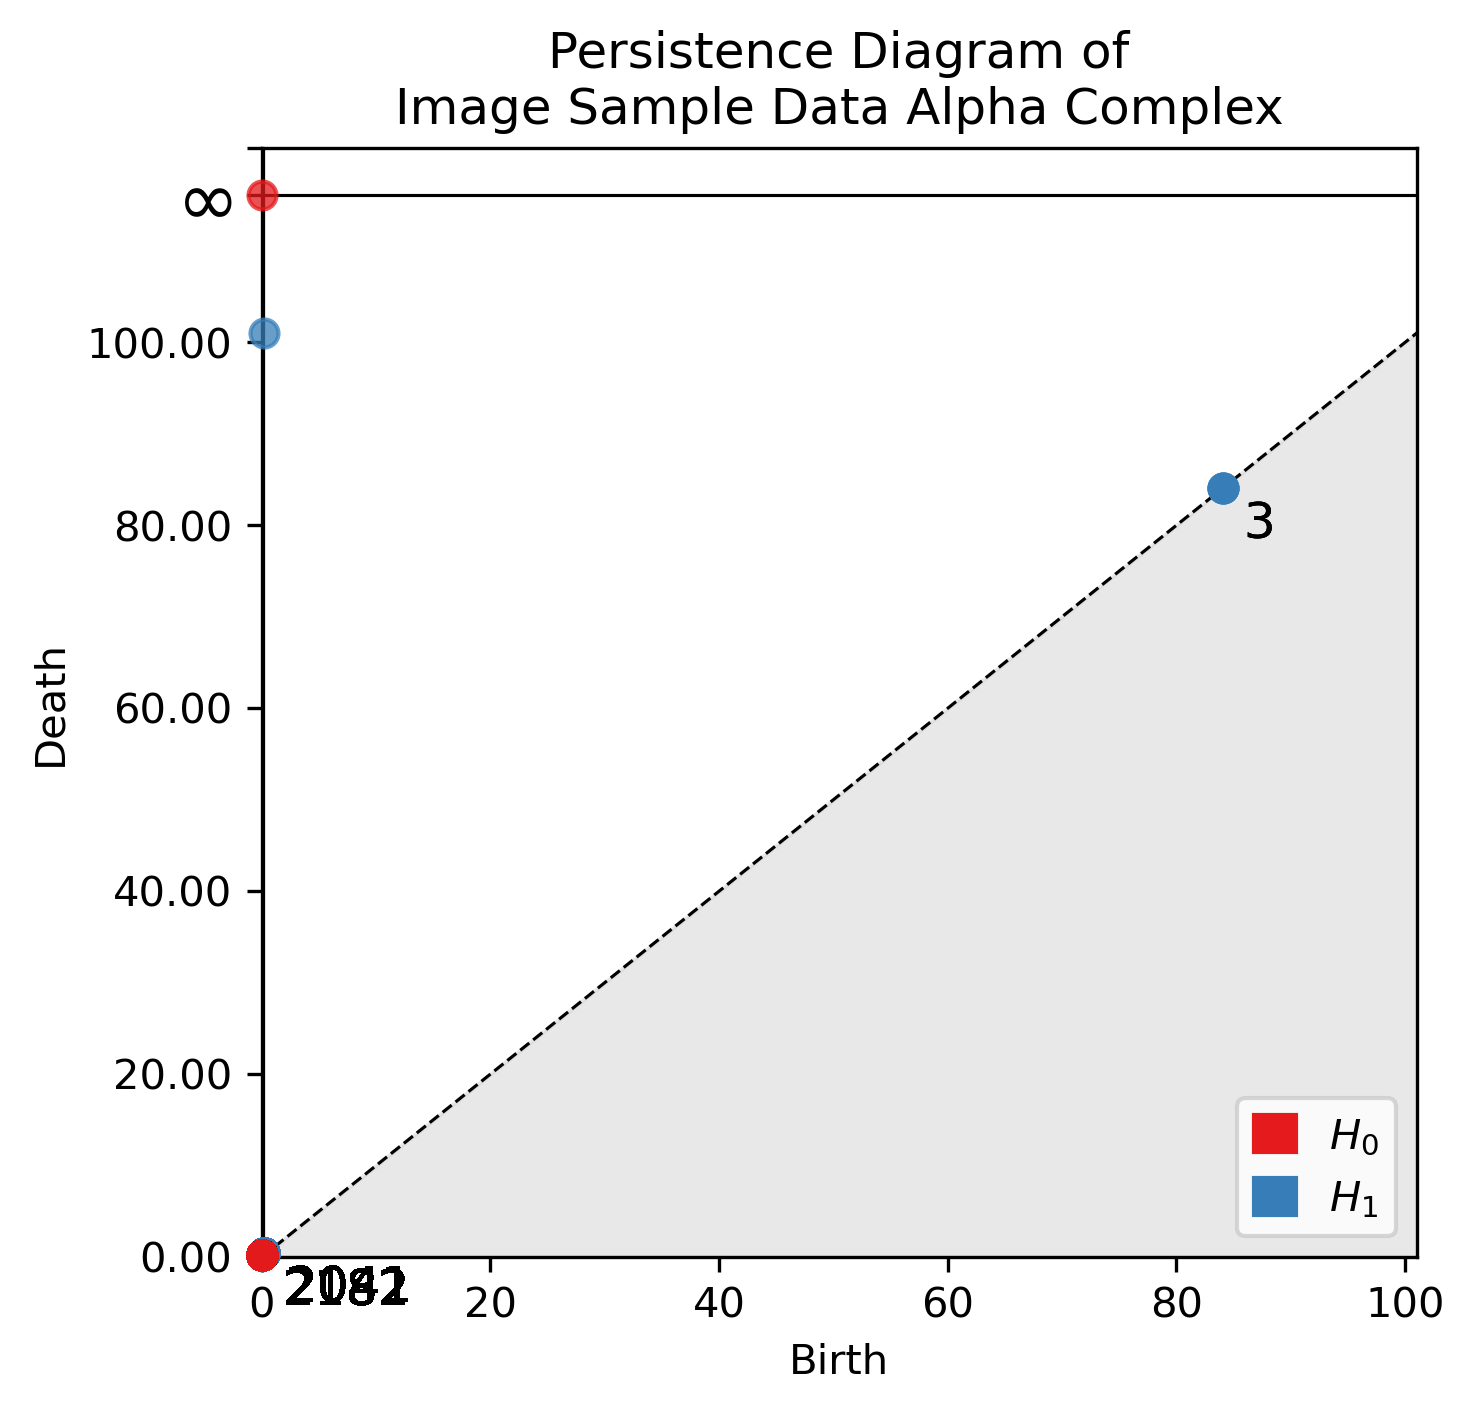
\includegraphics[width=\textwidth]{image_data_persdia.png}
    \end{subfigure}
    \caption{Plot of a white square with a hole and persistence diagram of its Alpha Complex.}
    \label{fig:image_data_persdia}
\end{figure}
\end{example}

\newpage
\section{Triangulation}
\par The Alpha complex is the ideal filtered simplicial complex to use when analyzing the homology of 3D objects as it can show us when connected components and holes are born and die in the persistent homology of the object. This is possible in part due to the Delaunay triangulation, but an alternative method, the Constrained Delaunay Triangulation, will be used in its place to achieve the best possible results.

delaunay complex is formed by intersection of voronoi cells regarldess of original edges

\begin{definition}[Constrained Delaunay Triangulation]
\label{def:cdt}
 \cite{chew1987constrained}
\end{definition}

\begin{definition}[Gabriel]
empty circumsphere means gabriel \cite{gabriel} circle around 
\end{definition}

\begin{figure}[H]
    \begin{center}
    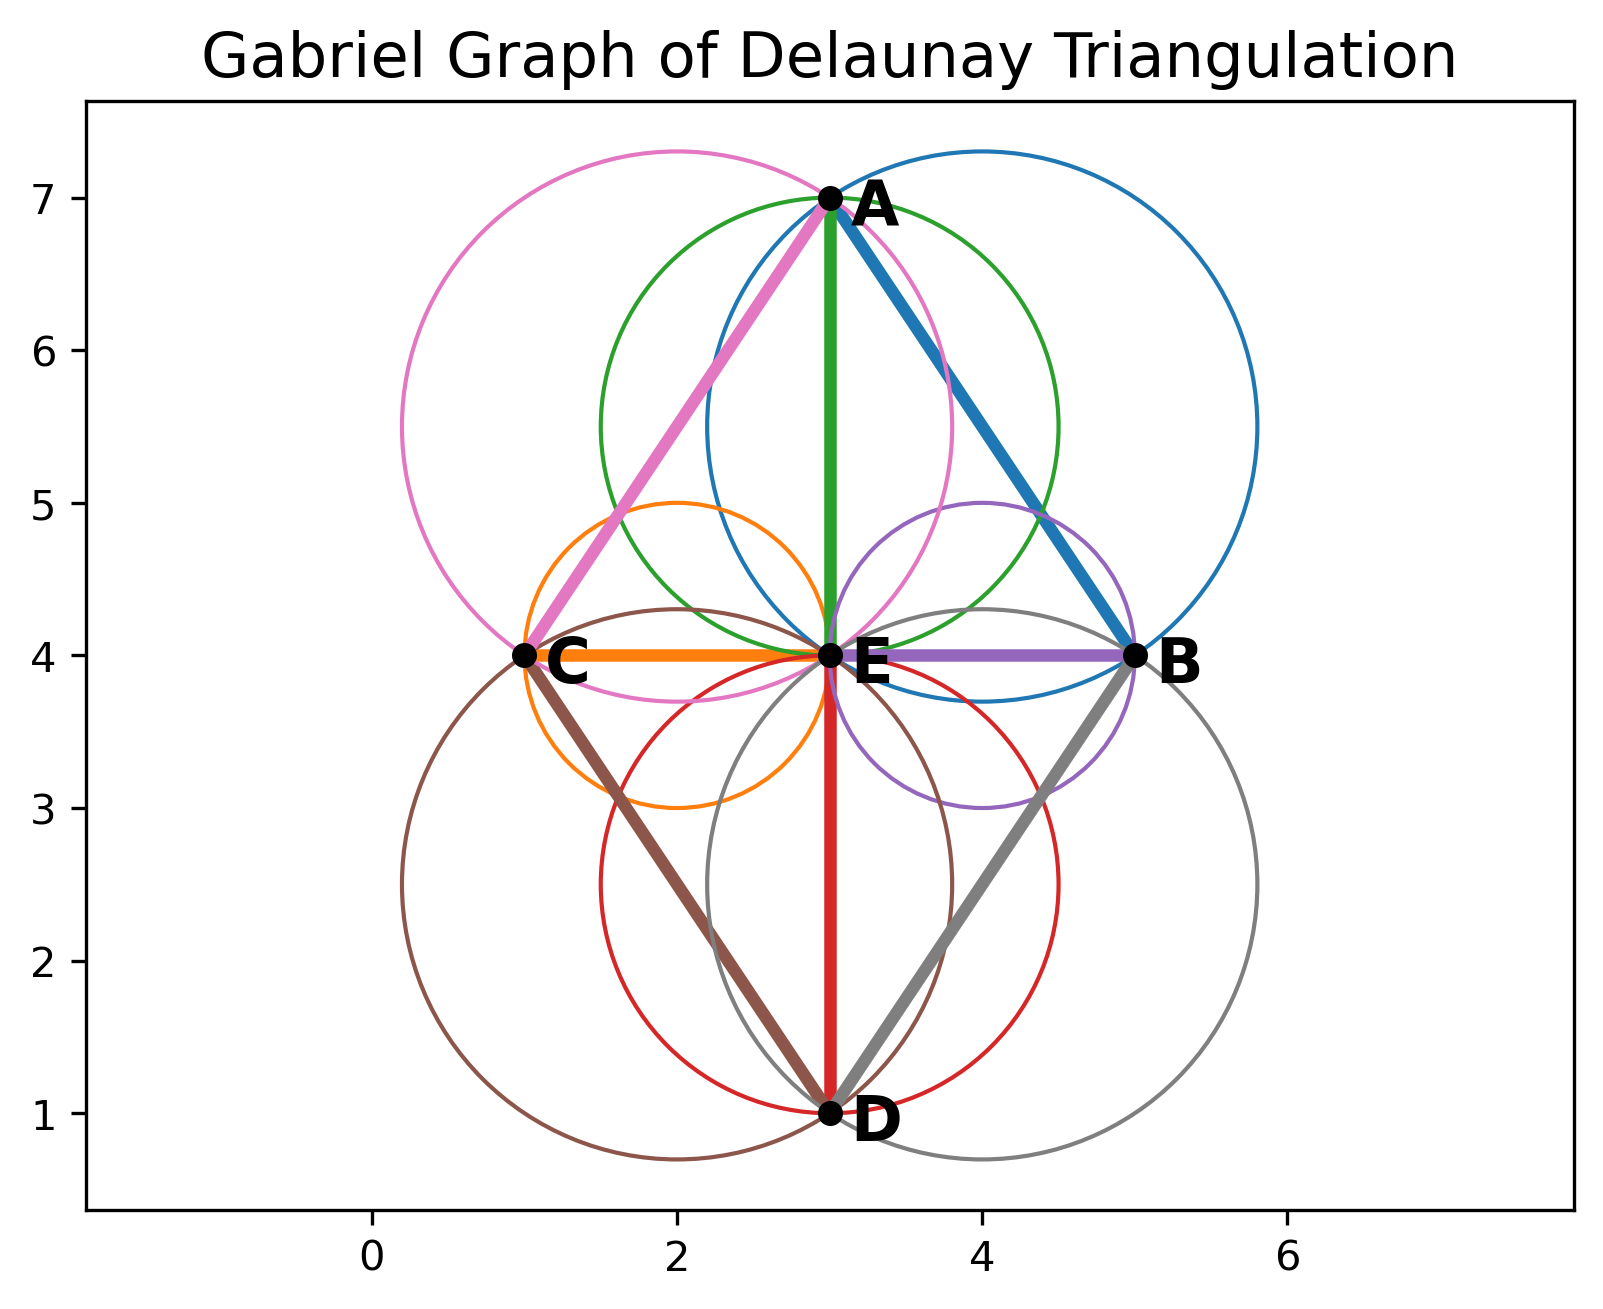
\includegraphics[width=0.55\textwidth]{gabriel_circles.png}
    \caption{Gabriel graph applied to a Delaunay triangulation of random points.}
    \label{fig:ast_tetrahedron}
    \end{center}
\end{figure}

\newpage
\section{Background on the STL Filetype}
An STL file is a filetype created for use with 3D data generated by computer-aided design (CAD) programs for 3D printing and other rapid-prototyping applications. STL is ancronym which can be an abbreviation for Stereolithography, Standard Triangle Language, or Standard Tesselation Language. These files are built through triangulation: every set of points creates a triangle which acts as a facet of the object. These triangles are 'filled-in' 2-simplices, and will be fundamental in analyzing the topology of STL files. In terms of the contents of an ASCII STL file, a facet should not be confused with a face: a facet must be a triangle, while a face of a polyhedron can be subdivided into multiple facets to achieve triangulation. The information in an STL file can be encoded using binary or in ASCII as a .ast (ASCII STL) file. For our purposes, we will be using .ast files to extract and analyze 3D object data. \cite{analysis_of_stl}

\begin{figure}[H]
    \begin{center}
    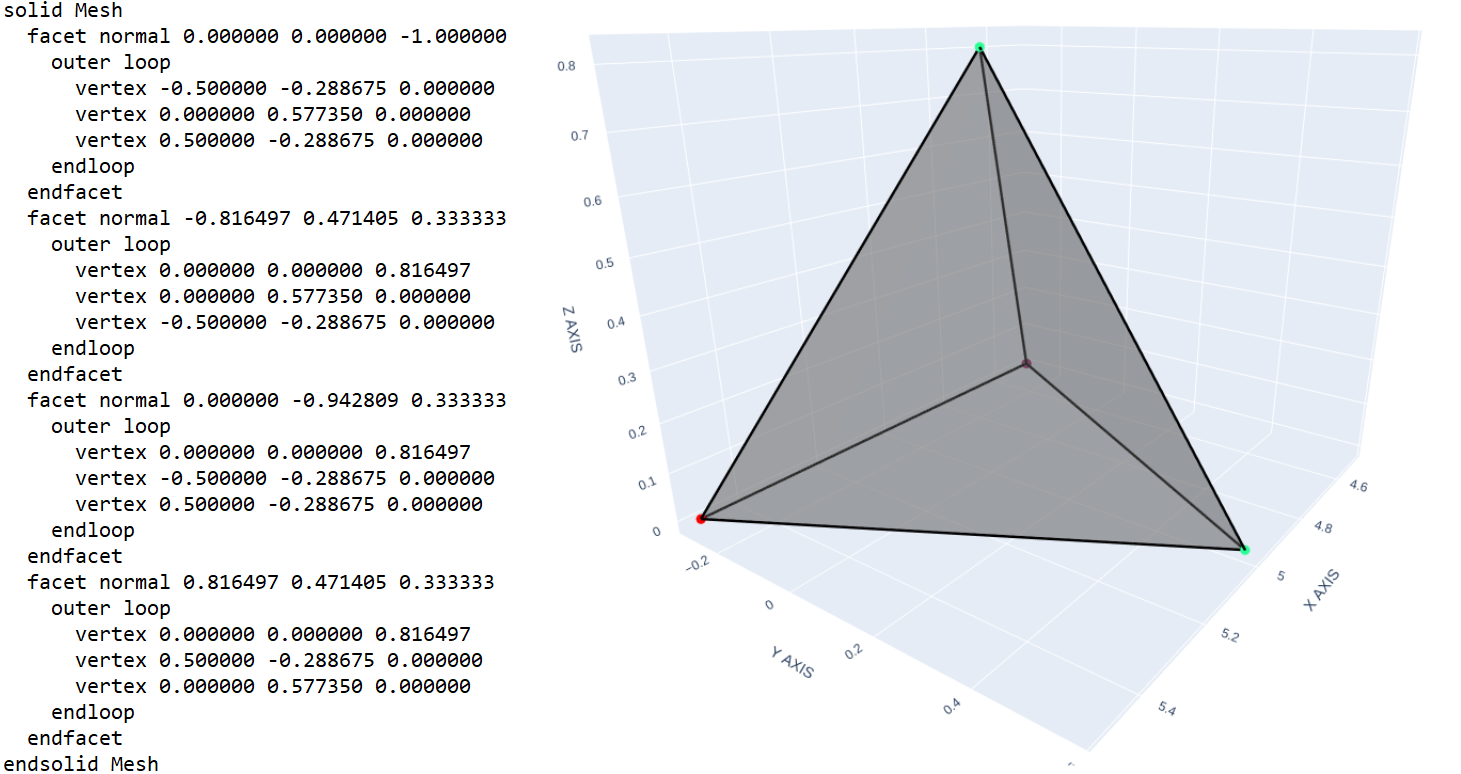
\includegraphics[height=2.9in]{tetrahedron_ast_code_and_plot.png}
    \caption{The contents and 3D plot of an ASCII STL file for a tetrahedron.}
    \label{fig:ast_tetrahedron}
    \end{center}
\end{figure}
\vspace{-7.5mm}

STL files contain descriptions of individual vertices, each of which are encapsulated its facet with its normal vector, as seen in the example tetrahedron, Fig \ref{fig:ast_tetrahedron}. The contents of an STL file do not specify topological information, such as connections to other vertices, which vertices make up a face, etc. Instead, STL files describe each vertex as many times as it appears in the file until the overall shape is built.

To analyze the topological data within STL files, the .ast files are parsed for four strings which are used to denote the beginning and end of the description of facets and vertices: 'facet normal', 'end facet', 'outer loop', and 'end loop', respectively. The data between these strings was then converted into a tuple using python.


\chapter{Methods}\label{chap:methods}

explain method big good

\section{Main Method}
\subsection{Creating a Mesh from an STL file}
\par To compute the persistence of variations of the "truth" of an STL file, the data must be processed and transformed with meshing in order to be properly analyzed.
\par Although STL files contain a mesh upon being created, this mesh is not adequate for our purposes. The mesh an STL file creates is not necessarily a Delaunay triangulation, so we need to create a mesh that meets the requirements of being Gabriel with a Constrained Delaunay Triangulation (CDT, see Def \ref{def:cdt}). 


\subsection{Creating and modifying an Alpha Complex}
\par Creating modified alpha complex (refer to background) by adjusting filtration values to 0 when 

\subsection{Computing a Persistence Diagram}

\section{Implementation}

\subsection{Creating STL Files with FreeCAD}

\par STL files from online sources such as Thingiverse can be processed as well but as mentioned earlier, these files may be too complex and therefore very computationally expensive. 

\subsection{Parsing the STL File Data}

\cprotect\subsection{Creating a Constrained Delaunay Triangulation with \verb+meshpy+}

\par \verb"MeshPy" is a using \verb"tetgen" \cite{tetgen}

\subsubsection{Switch '-p'}
Tetrahedralizes a piecewise linear complex (PLC).

\subsubsection{Switch '-D'}
An option for the \verb"'p'" switch to generate a constrained Delaunay tetrahedralization.

\subsubsection{Switch '-q'}
Refines mesh to improve mesh quality

\cprotect\subsection{Creating and Modifying an Alpha Complex with \verb+gudhi+}
\par Now that we have a Delaunay triangulation mesh, we are ready to generate an Alpha Complex wihth \verb"gudhi"  - recall that every simplex in alpha complex is delaunay/gabriel therefore every simplex present in the triangulation is somewhere in alpha copmlex.
\par We need delauney triangulation so every simplex appears in alpha complex. The alpha complex can grow to include simplices which were not originally in the CDT mesh created by \verb"meshpy". The simplices will be compared with the CDT to check for which simplices were originally in the triangulation: all simplices that were originally present will be given a filtration of 0, indicating a birth time of $b=0$, while all other simplices will retain their assigned filtration.
a
\cprotect\subsection{Filtration Construction with \verb+gudhi+}
\par \verb"Gudhi" is a
change filtration so that every original simplex has a filtration value of 0 so it appears in $K_{0}$

\subsection{Persistence Diagram Construction}
\par 

\begin{example}
picture of cad object, then mesh, then persistence diagram
\end{example}

\chapter{Results}
\section{Two Cubes with Three Pockets Moving Closer}
\begin{multicols}{2}
A CAD pocket operation subtracts an area from a face. This can also create a hole which goes through an object's face. This operation was done to a cube on the top, front, and right faces to create three intersecting pockets through each face of the cube, as shown in \ref{fig:three_pocket_example}.
\columnbreak
\begin{figure}[H]
\begin{center}
	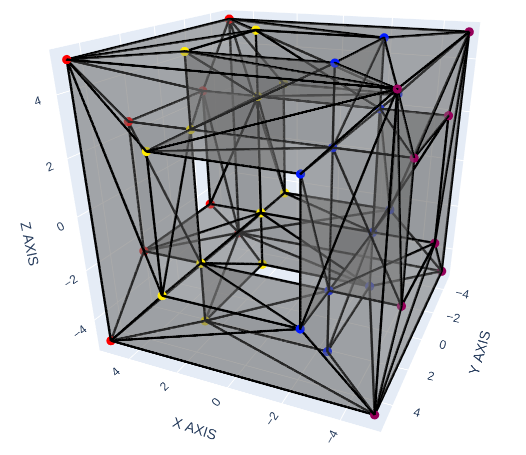
\includegraphics[height=1.1in]{one cube three pockets each.png}
    \caption{Cube with three pockets.}
\label{fig:three_pocket_example}
\end{center}
\end{figure}
\end{multicols}
\vspace{-7.5mm}
\begin{table}[H]
    \begin{center}
    \begin{tabular}{|c|c|}
    \toprule
    \tstack{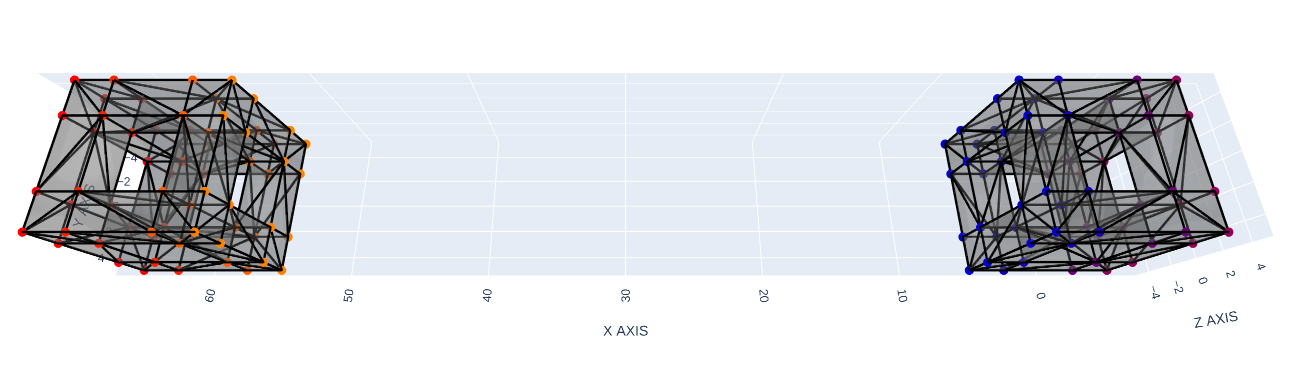
\includegraphics[height=0.75in]{Final Run, (two cubes, three pockets each, 50 mm apart) meshpy plotly screenshots.png}\\ {\fontsize{10}{12}\selectfont 50 mm apart}}  &
    \tstack{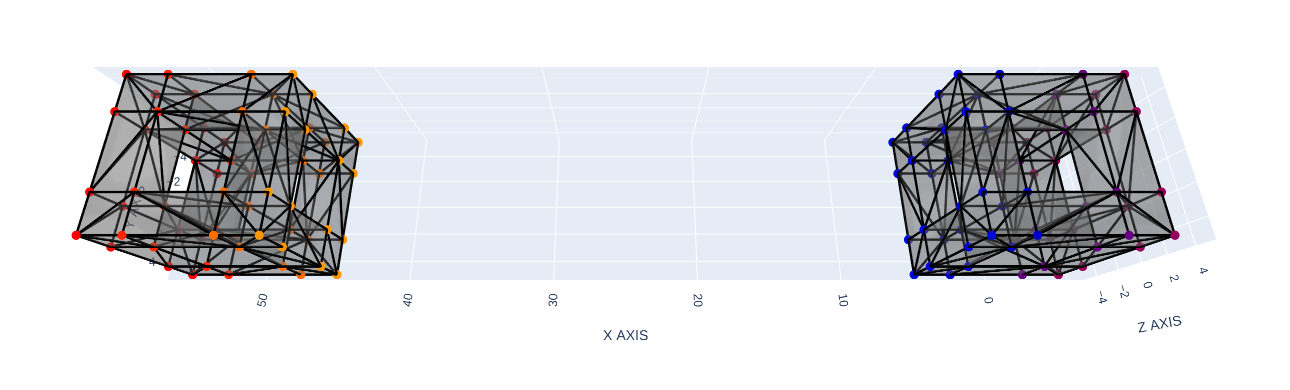
\includegraphics[height=0.75in]{Final Run, (two cubes, three pockets each, 40 mm apart) meshpy plotly screenshots.png}\\ {\fontsize{10}{12}\selectfont 40 mm apart}}  \\
    \midrule
	\tstack{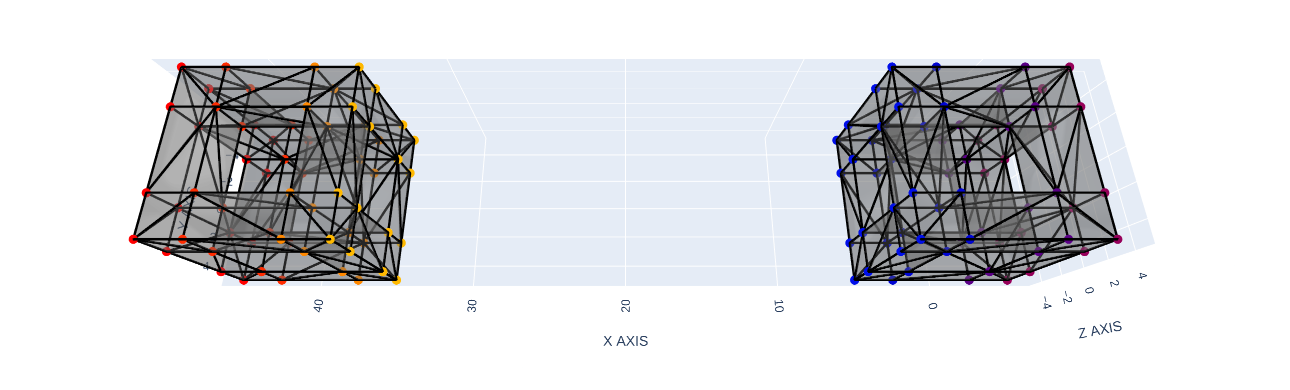
\includegraphics[height=0.75in]{Final Run, (two cubes, three pockets each, 30 mm apart) meshpy plotly screenshots.png}\\ {\fontsize{10}{12}\selectfont 30 mm apart}}   &
	\tstack{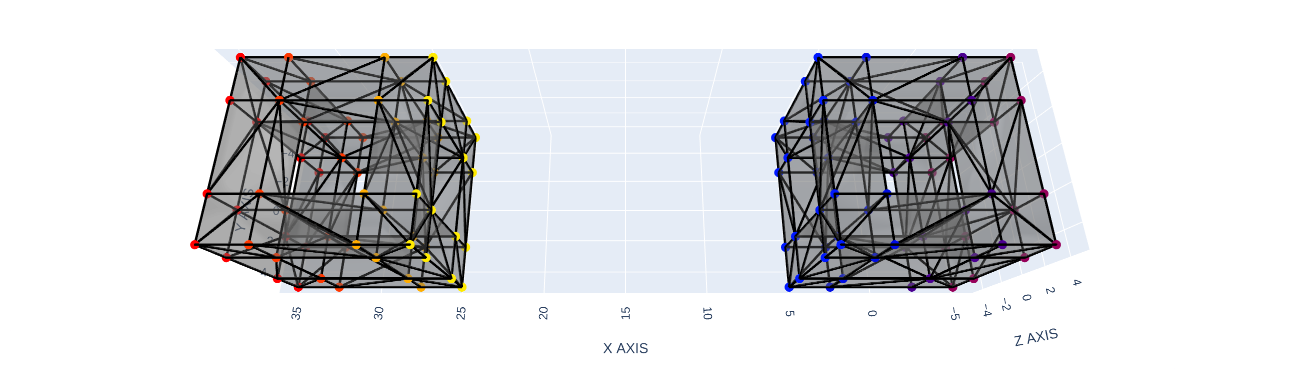
\includegraphics[height=0.75in]{Final Run, (two cubes, three pockets each, 20 mm apart) meshpy plotly screenshots.png}\\ {\fontsize{10}{12}\selectfont 20 mm apart}}  \\
	\midrule
    \tstack{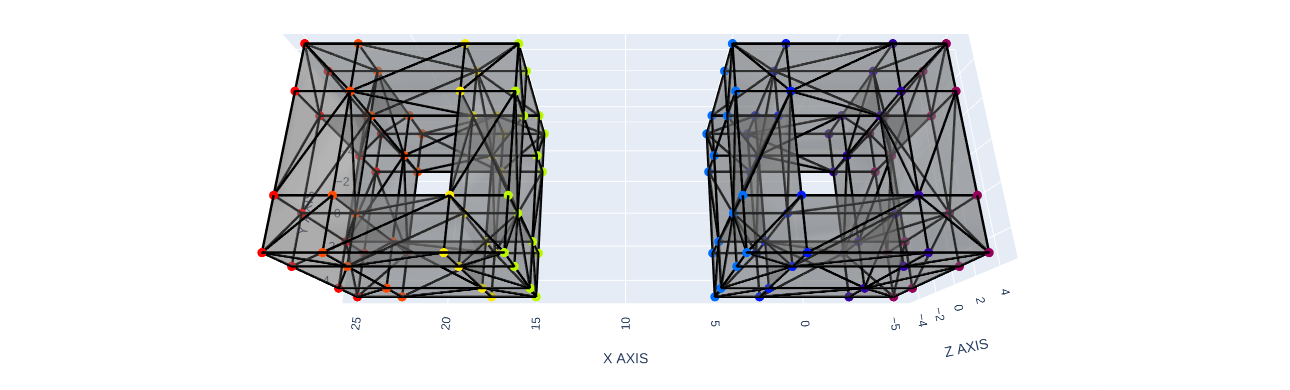
\includegraphics[height=0.75in]{Final Run, (two cubes, three pockets each, 10 mm apart) meshpy plotly screenshots.png}\\ {\fontsize{10}{12}\selectfont 10 mm apart}}  &
    \tstack{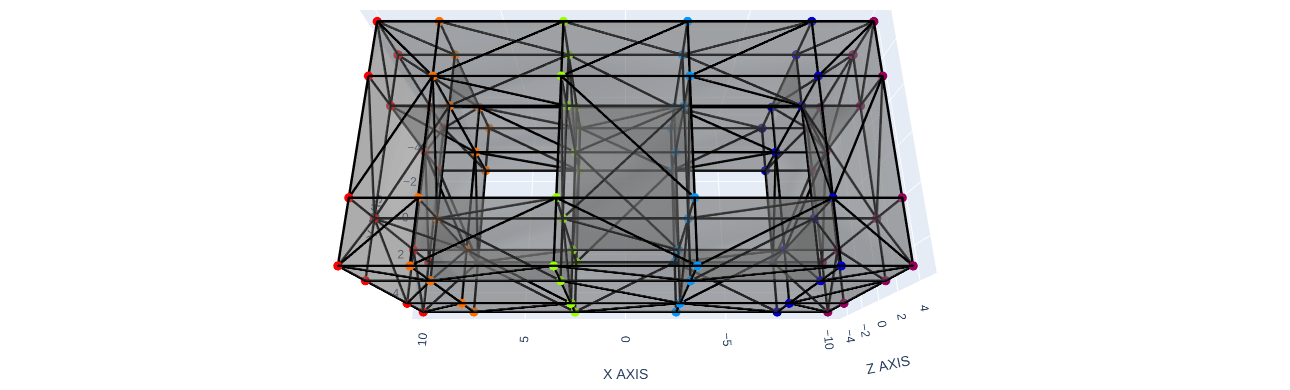
\includegraphics[height=0.75in]{Final Run, (two cubes, three pockets each, 00 mm apart) meshpy plotly screenshots.png}\\ {\fontsize{10}{12}\selectfont 00 mm apart}}  \\
    \bottomrule
    \end{tabular}
    \end{center}
    \caption{MeshPy Plots displayed with Plotly of two cubes with three CAD pocket operations that move closer together until combining.}
    \label{fig:cube_two_cubes_meshpy_table}
\end{table}

\begin{table}[H]
\begin{center}
    \begin{tabular}{cc}
         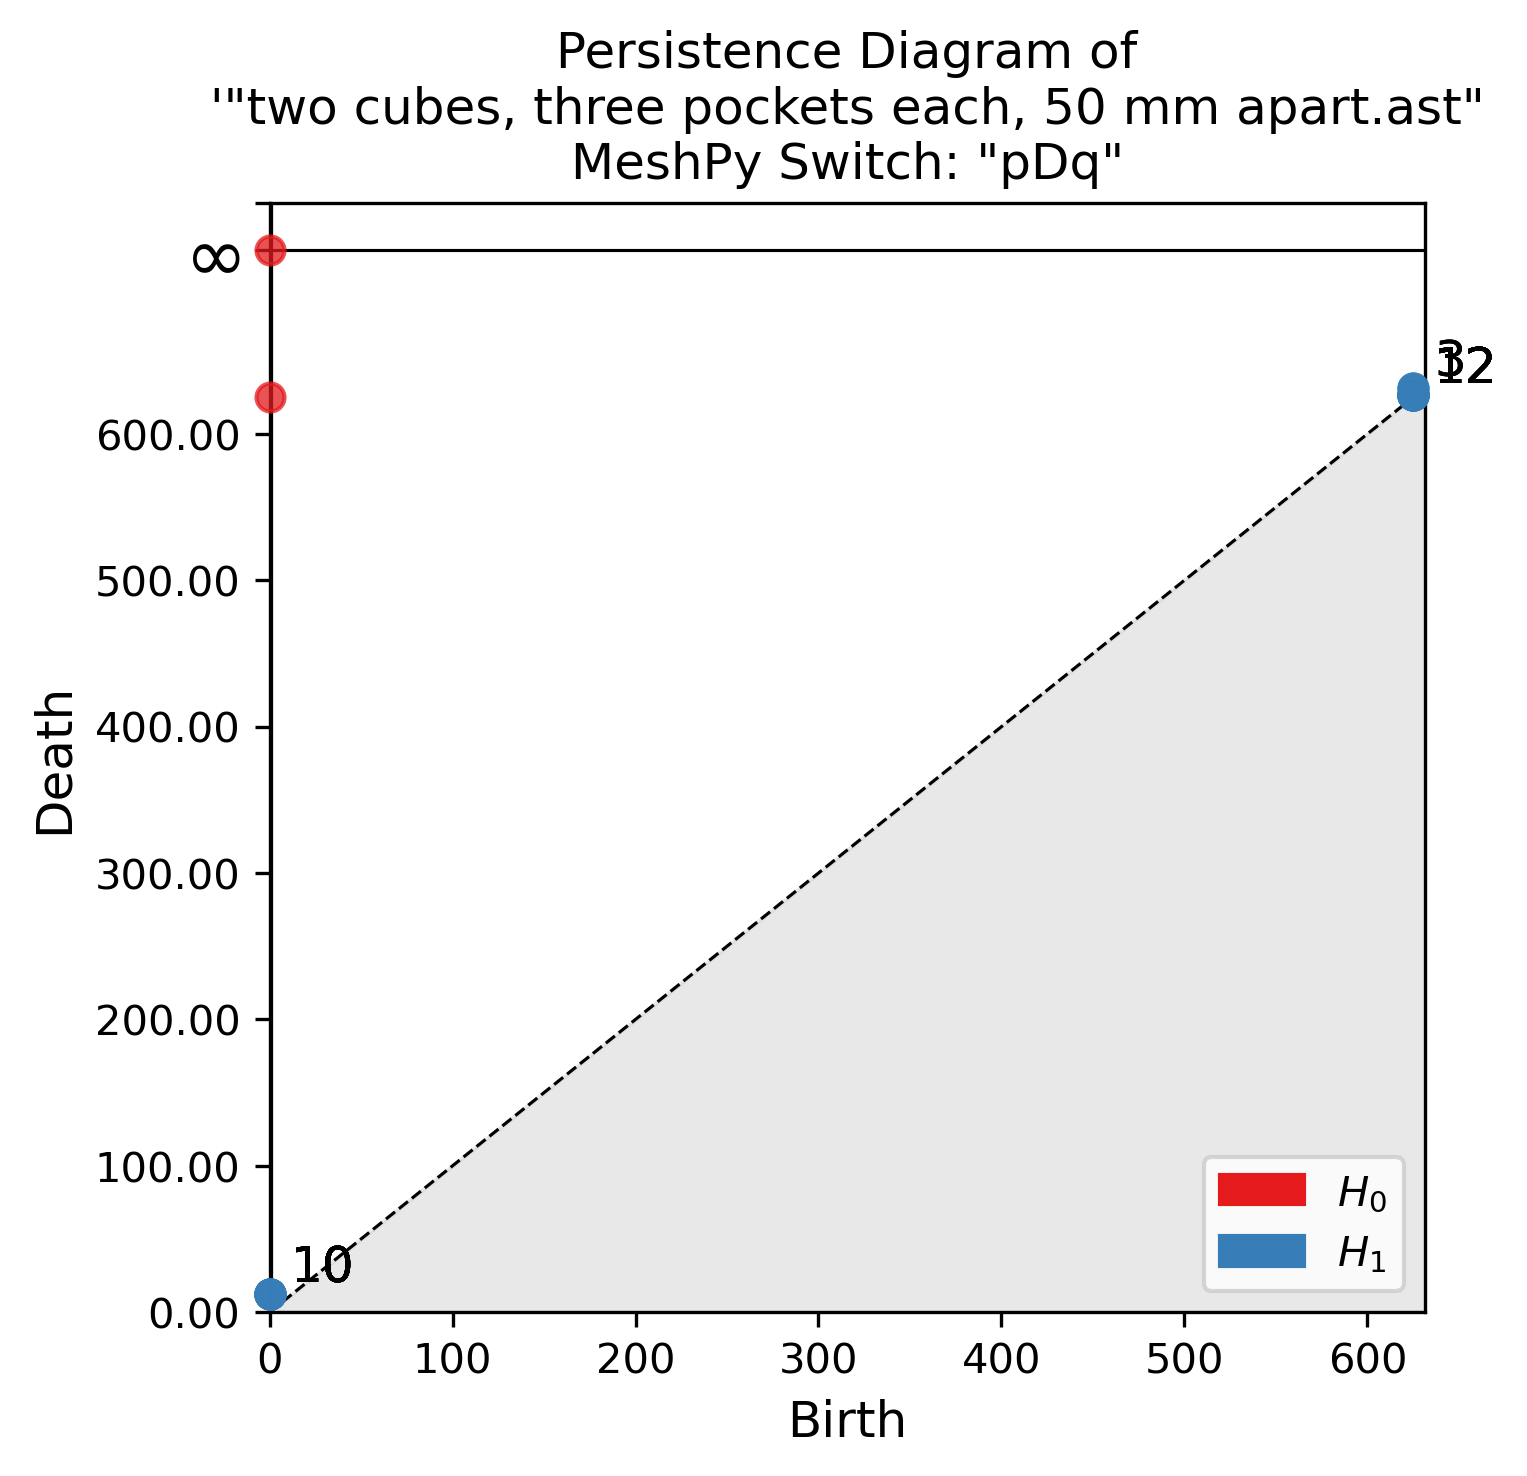
\includegraphics[width=2.5in]{Final Run, (two cubes, three pockets each, 50 mm apart) persdia.png} &
         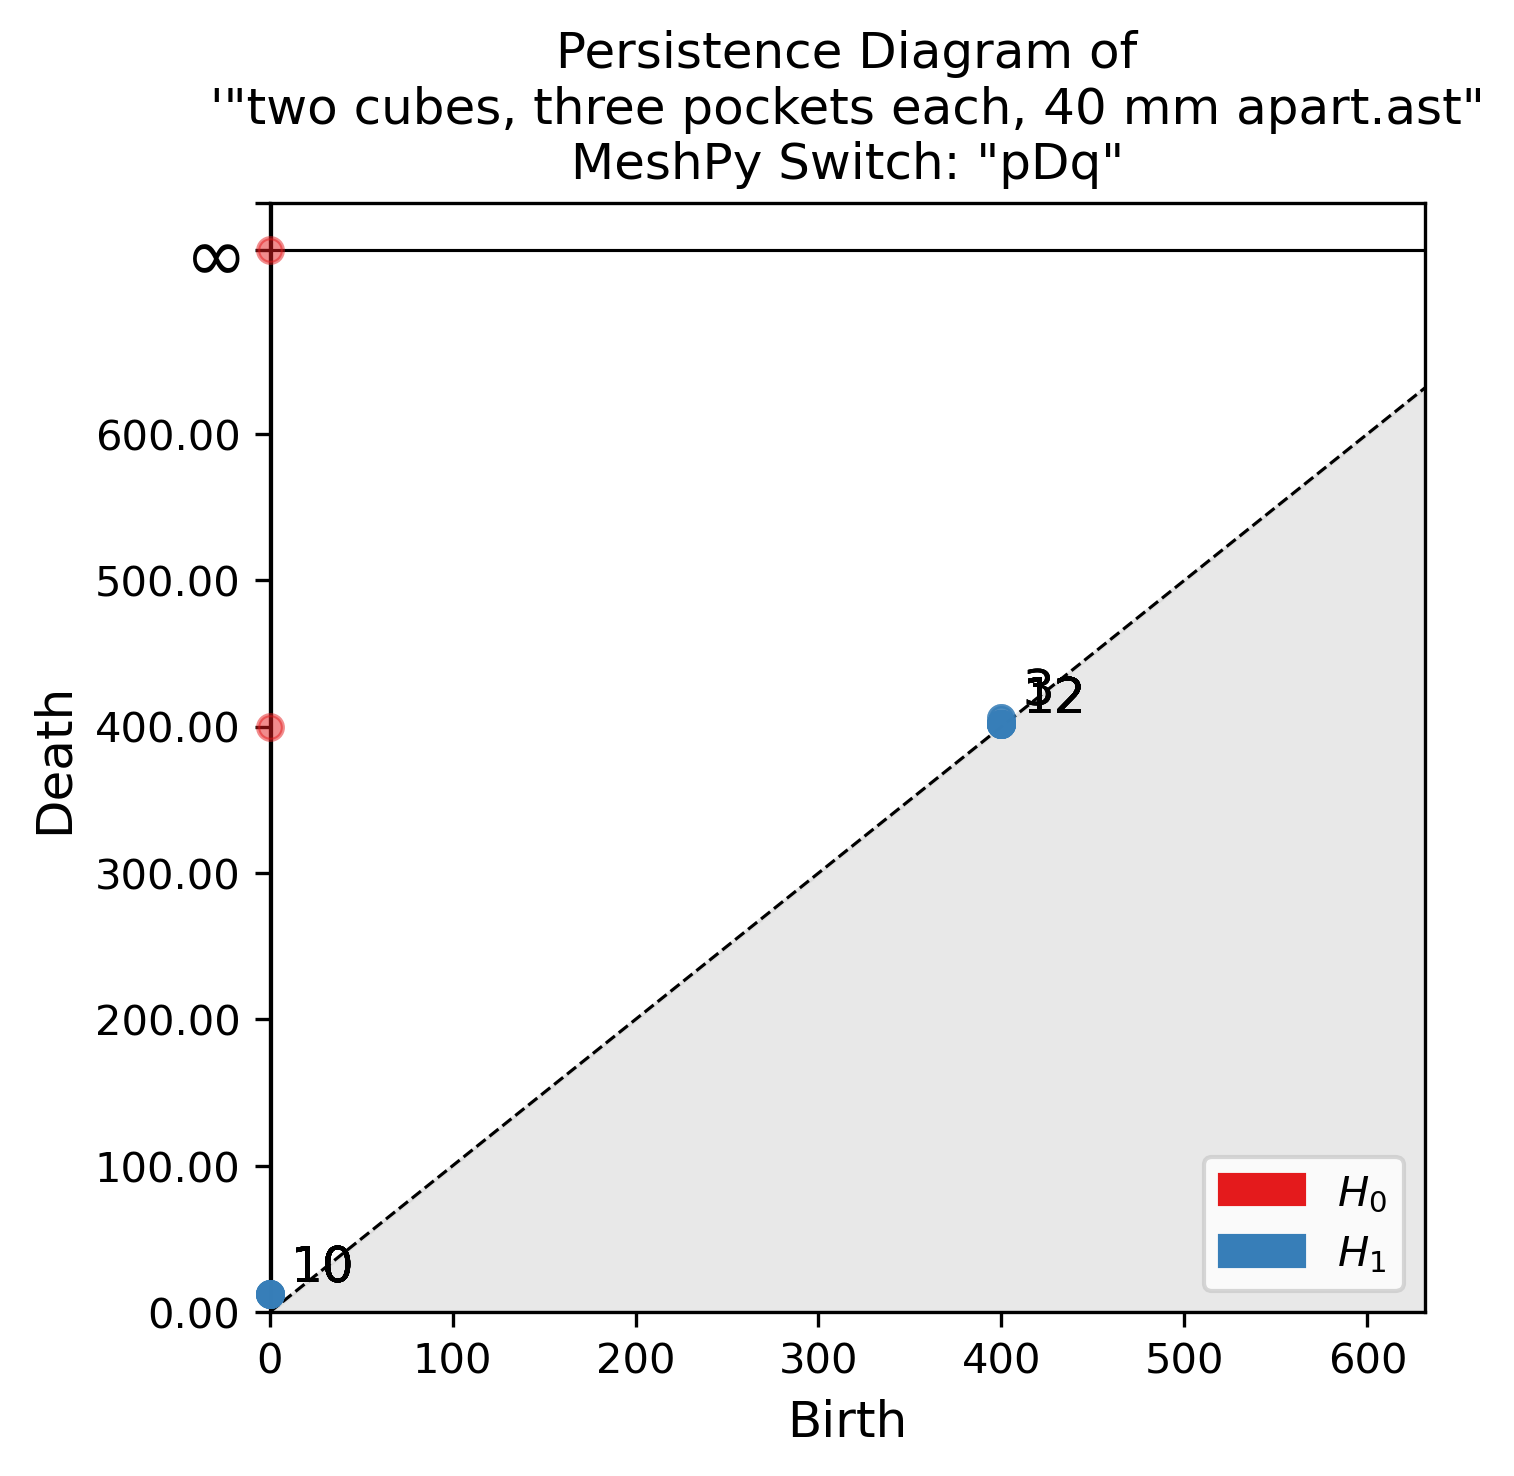
\includegraphics[width=2.5in]{Final Run, (two cubes, three pockets each, 40 mm apart) persdia.png} \\ 
         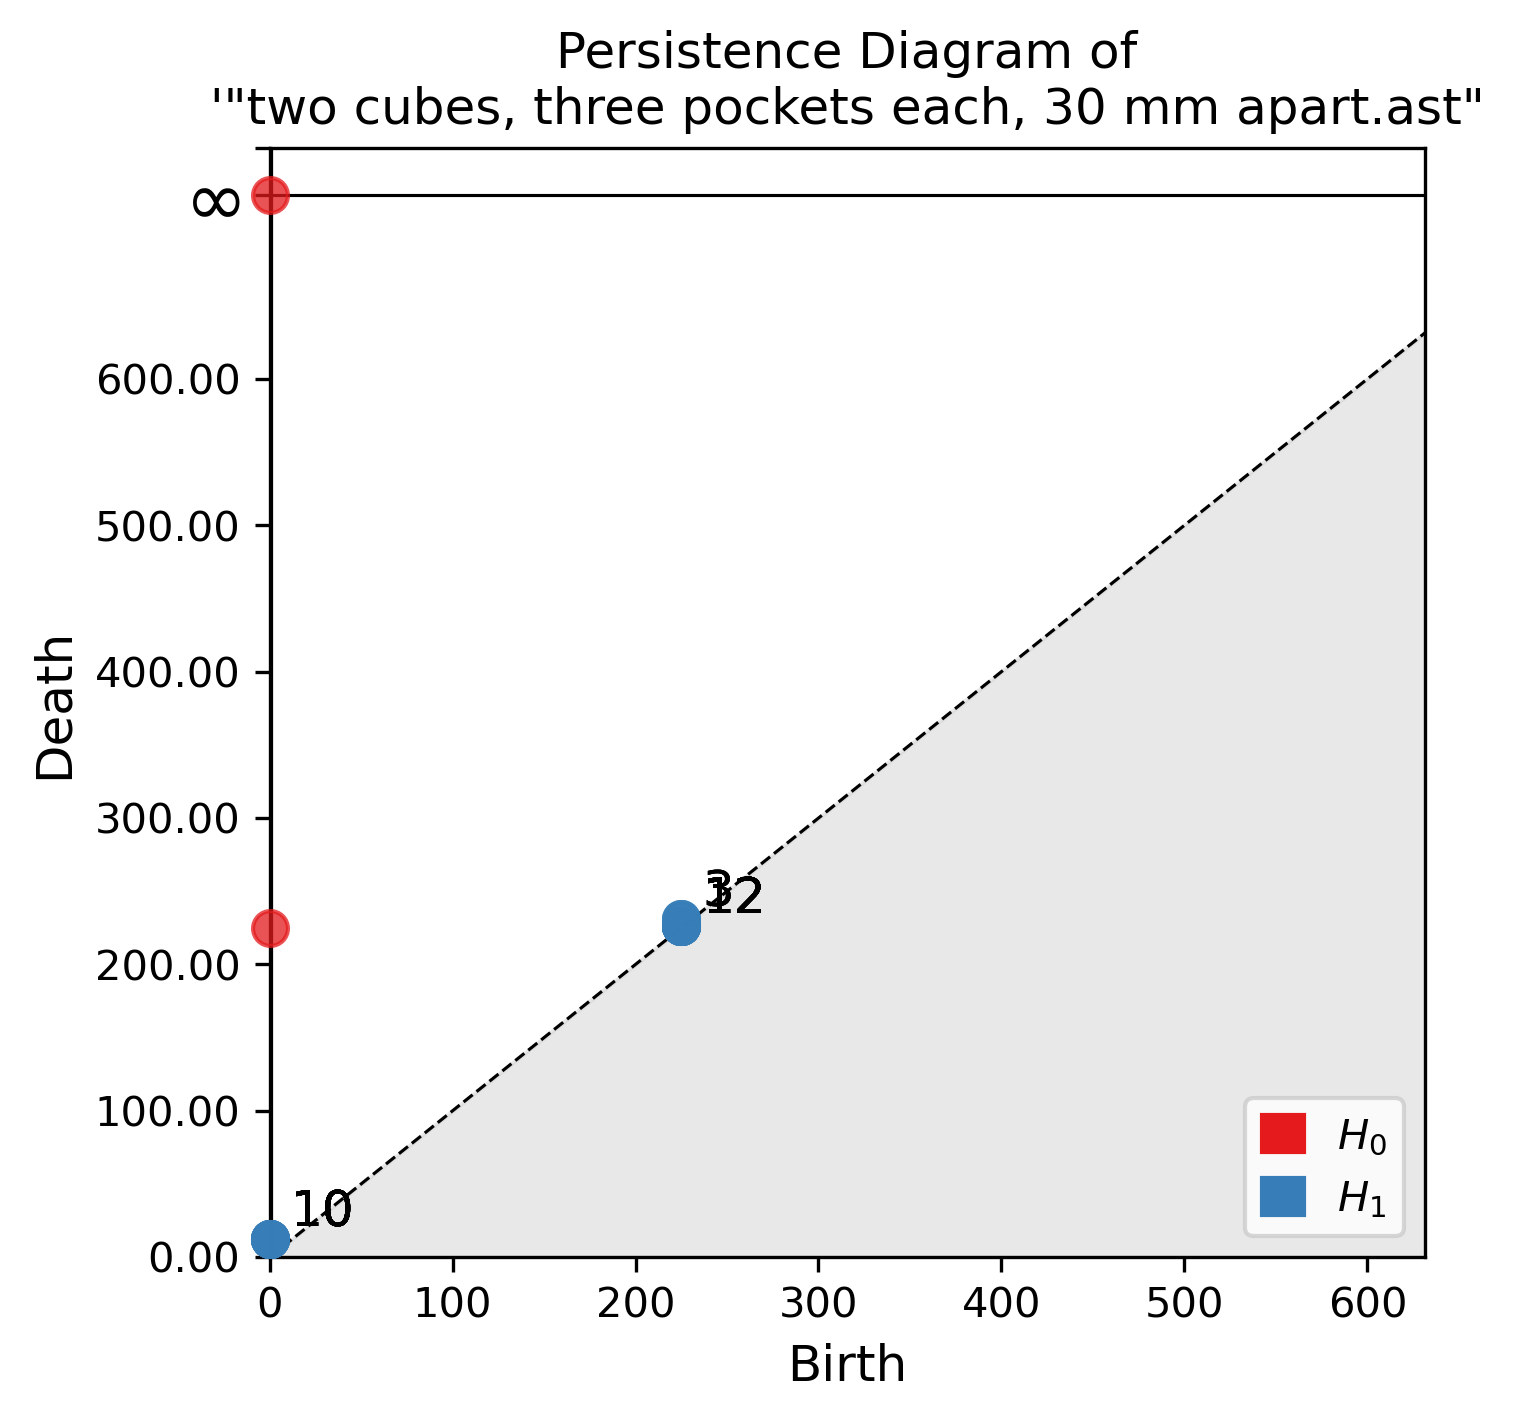
\includegraphics[width=2.5in]{Final Run, (two cubes, three pockets each, 30 mm apart) persdia.png} &
         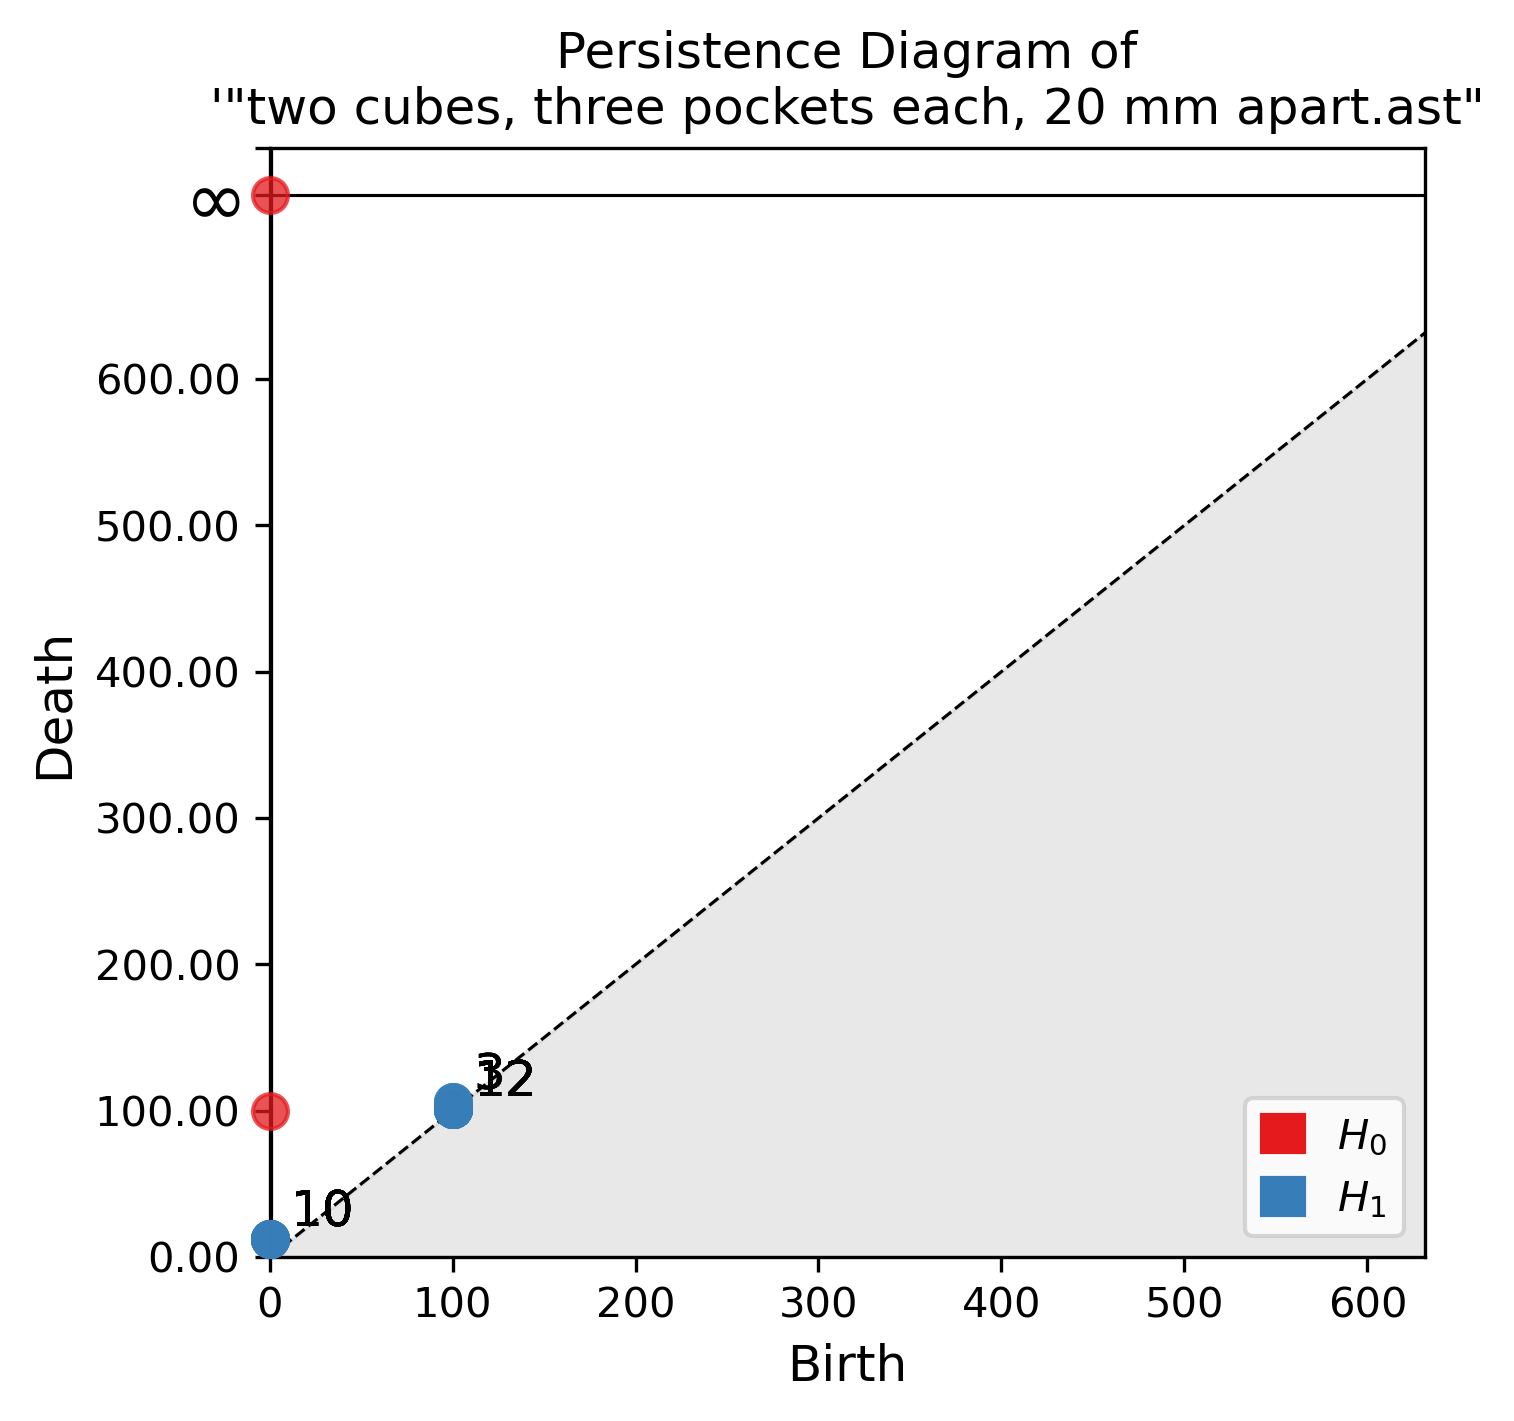
\includegraphics[width=2.5in]{Final Run, (two cubes, three pockets each, 20 mm apart) persdia.png} \\ 
         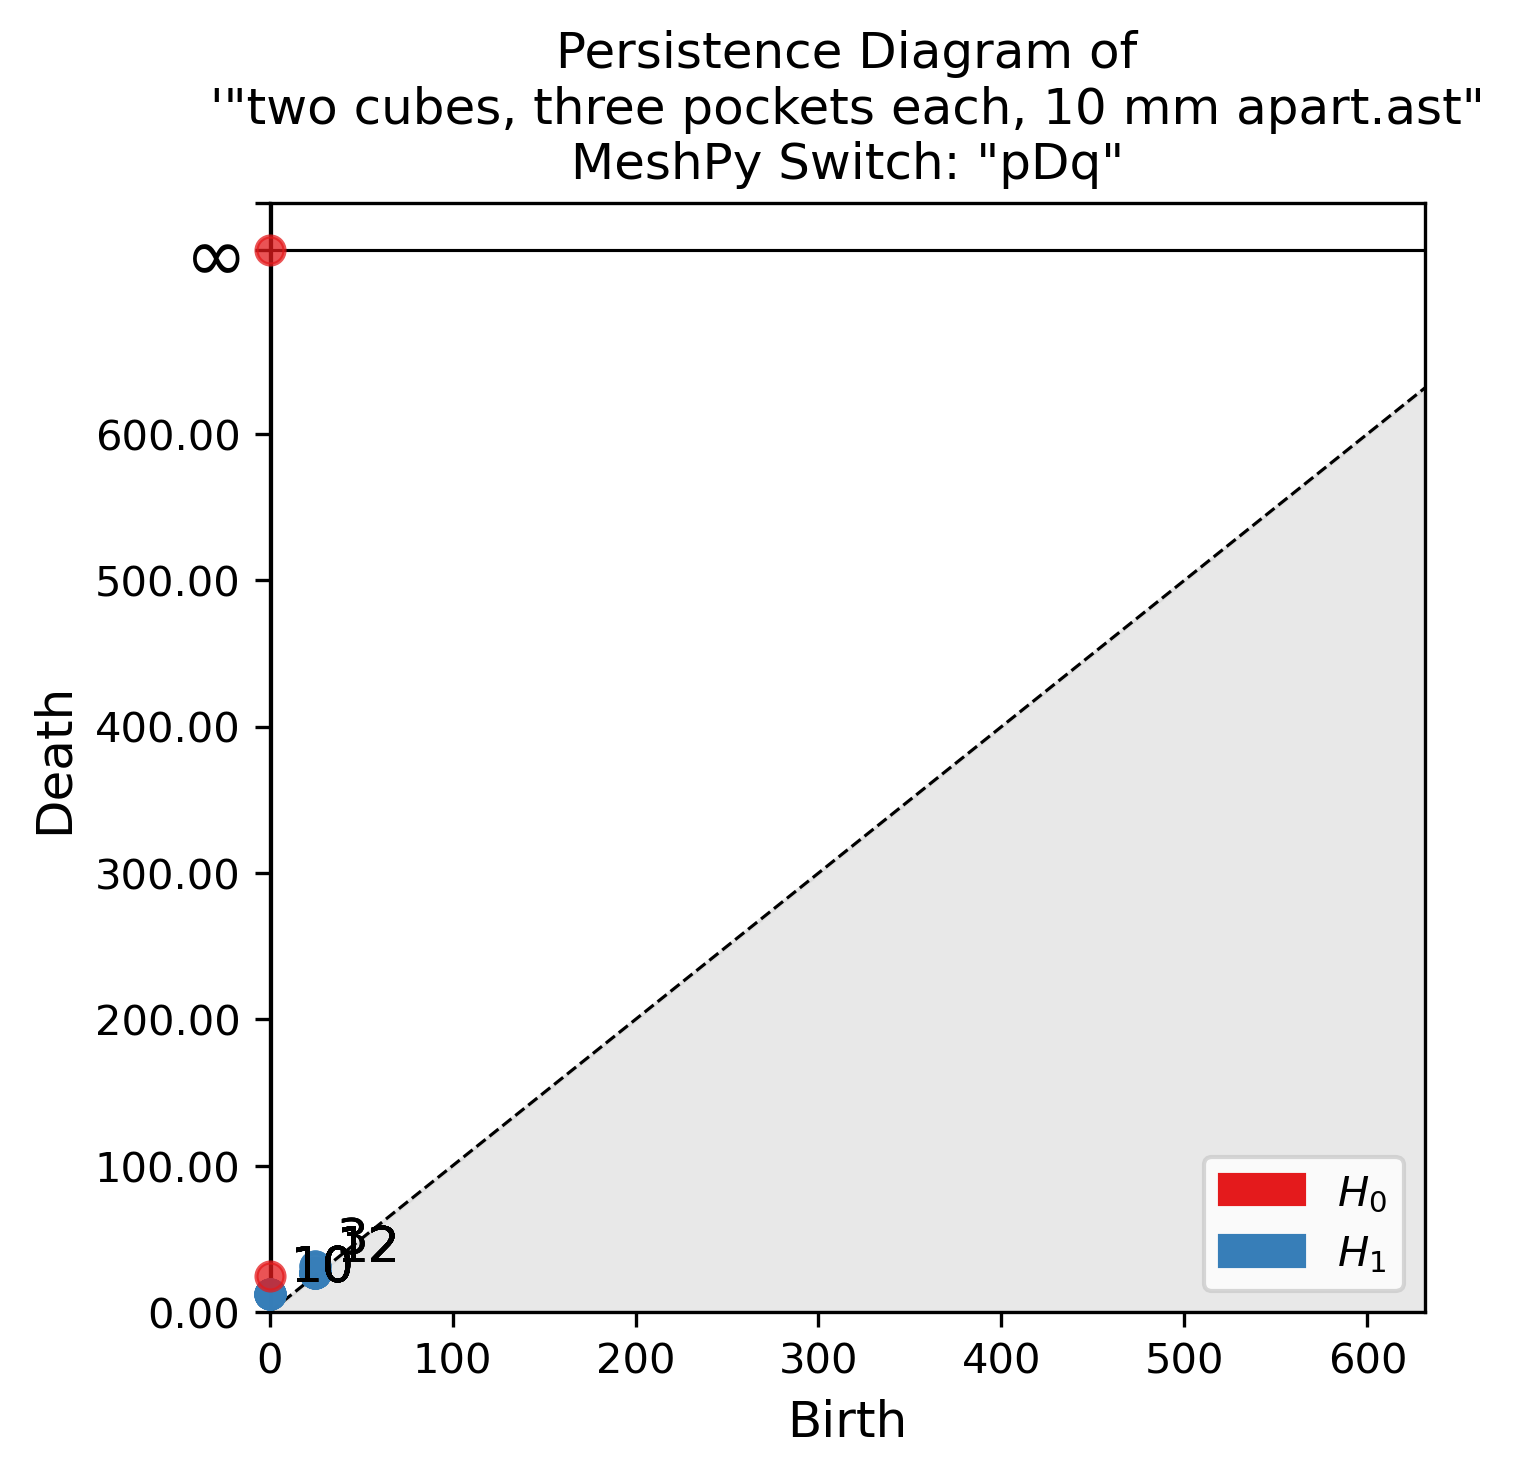
\includegraphics[width=2.5in]{Final Run, (two cubes, three pockets each, 10 mm apart) persdia.png} & 
         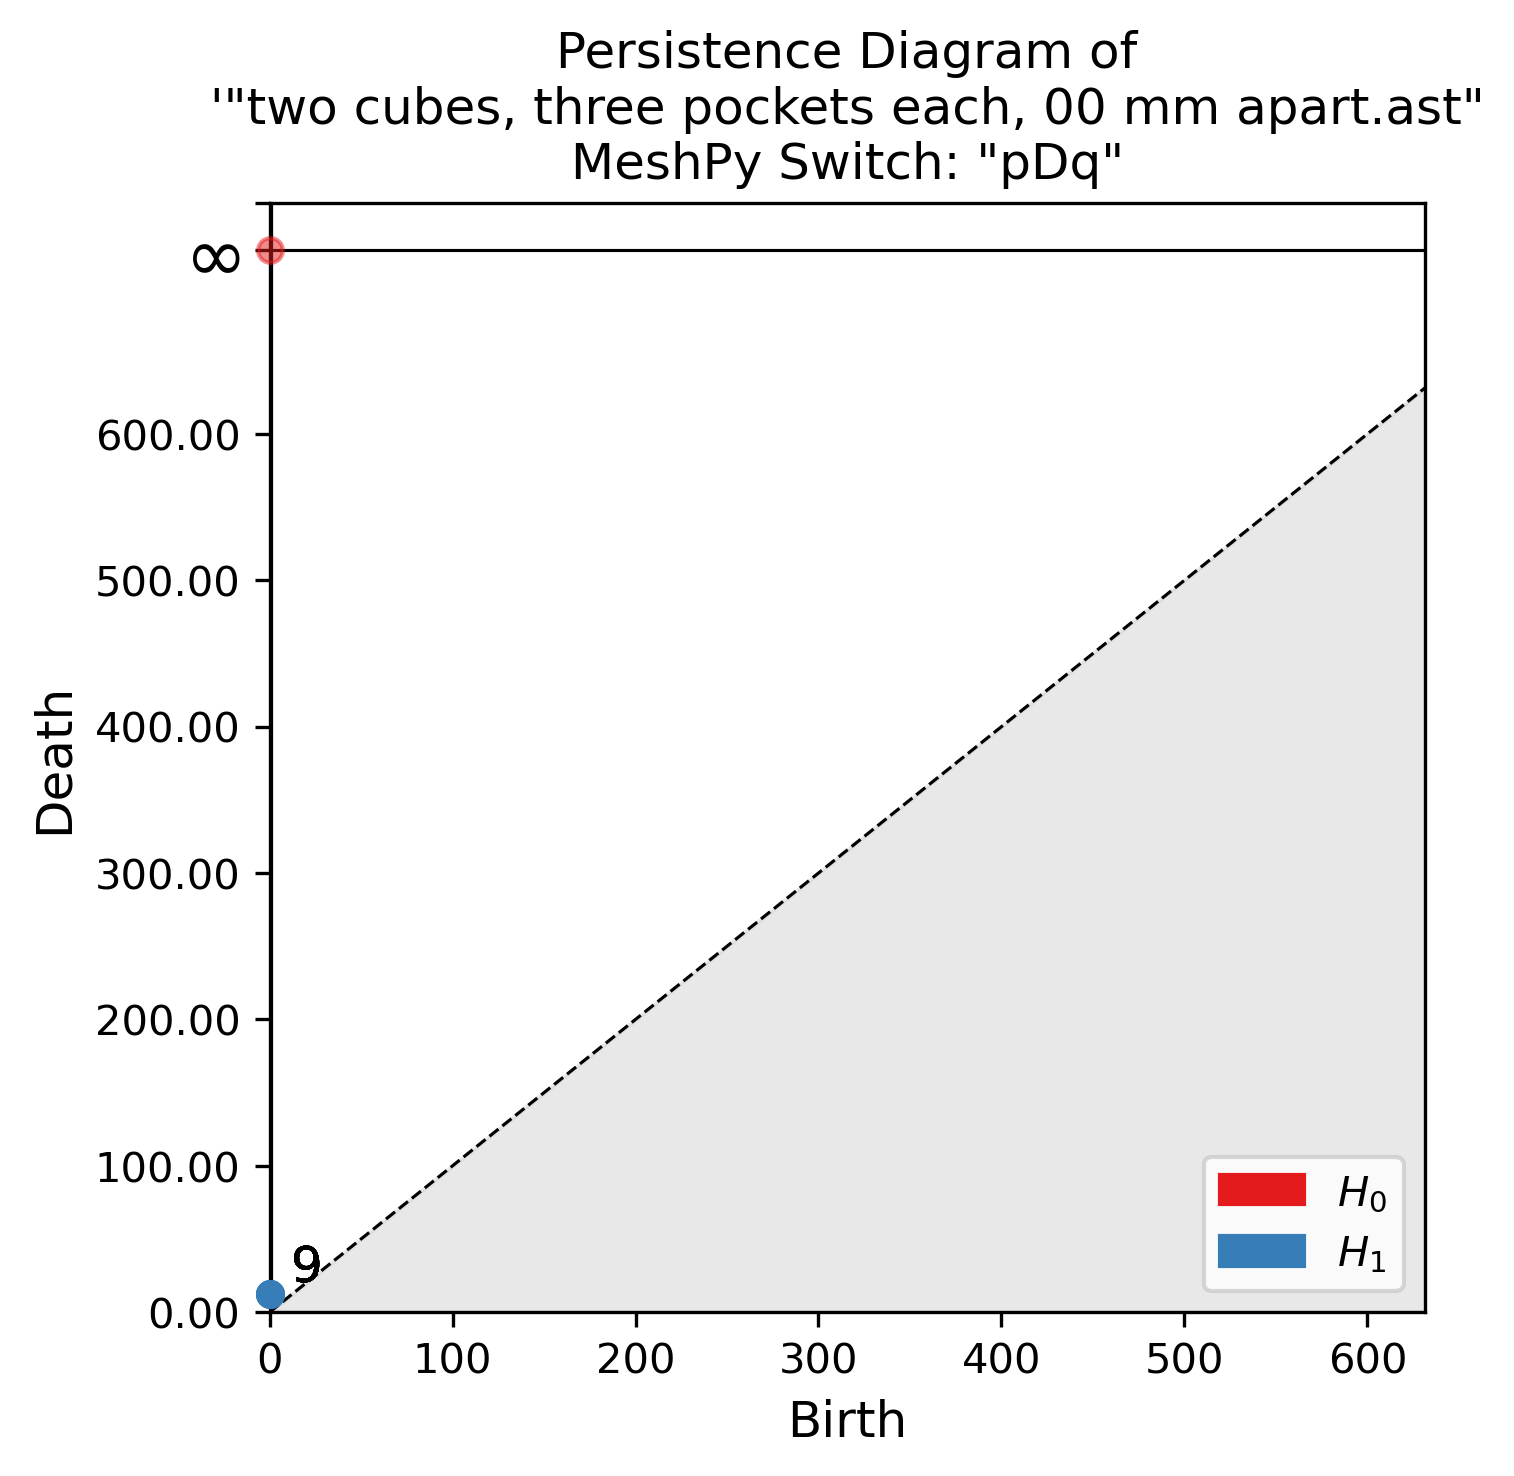
\includegraphics[width=2.5in]{Final Run, (two cubes, three pockets each, 00 mm apart) persdia.png} \\
\end{tabular}
\end{center}
    \caption{Persistence Diagrams of two cubes with three CAD pocket operations that move closer together until combining.}
    \label{fig:cube_two_cubes_persdia_table}
\end{table}

\subsection{Discussion}


\newpage
\section{Cube with Equilateral Triangle Hole}
An equilateral triangle was sketched onto the top face of a cube and a pocket operation was done through the cube. The equilateral triangle hole starts with an edge length of 8mm until it shrinks completely and dissapears.
\begin{table}[H]
	\begin{center}
    \begin{tabular}{|c|c|c|}
    	 \toprule
         \tstack{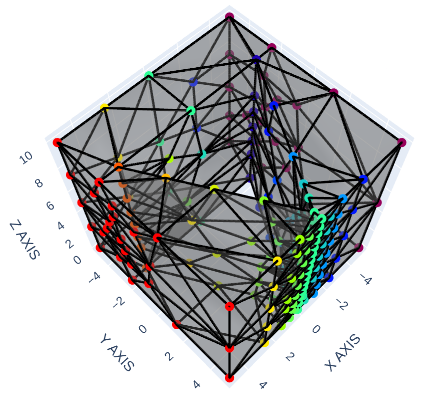
\includegraphics[width=1.75in]{Final Run, (cube - equilateral triangle hole 8 mm) meshpy plotly screenshot.png}\\ {\fontsize{10}{12}\selectfont Equilateral Triangle Hole, 8 mm}} &
         \tstack{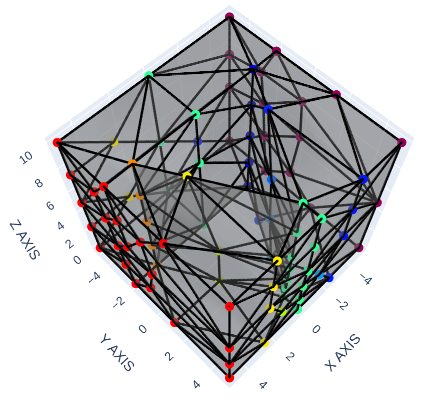
\includegraphics[width=1.75in]{Final Run, (cube - equilateral triangle hole 7 mm) meshpy plotly screenshot.png}\\ {\fontsize{10}{12}\selectfont Equilateral Triangle Hole, 7 mm}} &  
         \tstack{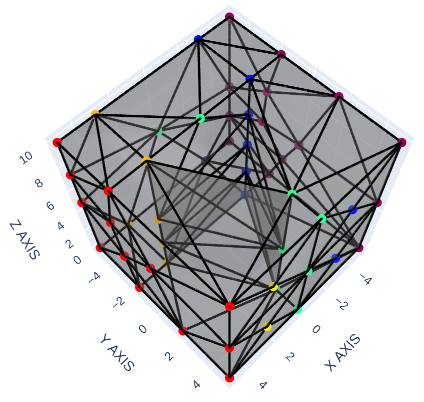
\includegraphics[width=1.75in]{Final Run, (cube - equilateral triangle hole 6 mm) meshpy plotly screenshot.png}\\ {\fontsize{10}{12}\selectfont Equilateral Triangle Hole, 6 mm}} \\
         \midrule
         \tstack{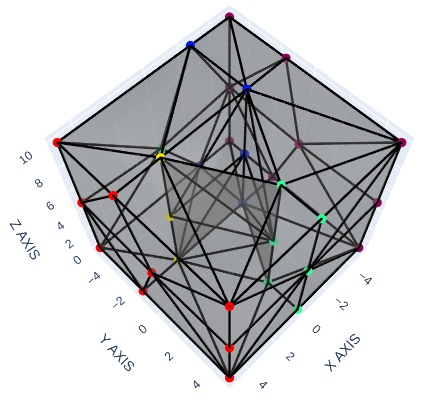
\includegraphics[width=1.75in]{Final Run, (cube - equilateral triangle hole 5 mm) meshpy plotly screenshot.png}\\ {\fontsize{10}{12}\selectfont Equilateral Triangle Hole, 5 mm}} & 
         \tstack{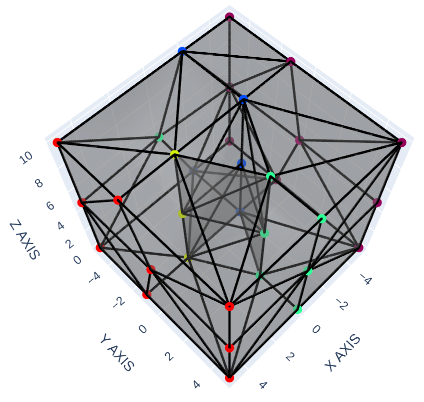
\includegraphics[width=1.75in]{Final Run, (cube - equilateral triangle hole 4 mm) meshpy plotly screenshot.png}\\ {\fontsize{10}{12}\selectfont Equilateral Triangle Hole, 4 mm}} & 
         \tstack{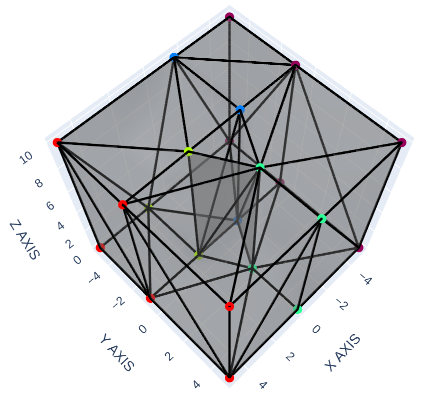
\includegraphics[width=1.75in]{Final Run, (cube - equilateral triangle hole 3 mm) meshpy plotly screenshot.png}\\ {\fontsize{10}{12}\selectfont Equilateral Triangle Hole, 3 mm}} \\
         \midrule
         \tstack{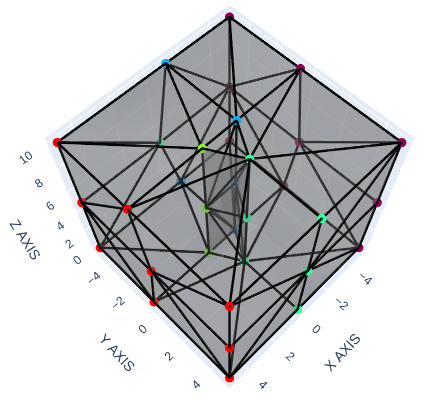
\includegraphics[width=1.75in]{Final Run, (cube - equilateral triangle hole 2 mm) meshpy plotly screenshot.png}\\ {\fontsize{10}{12}\selectfont Equilateral Triangle Hole, 2 mm}} & 
         \tstack{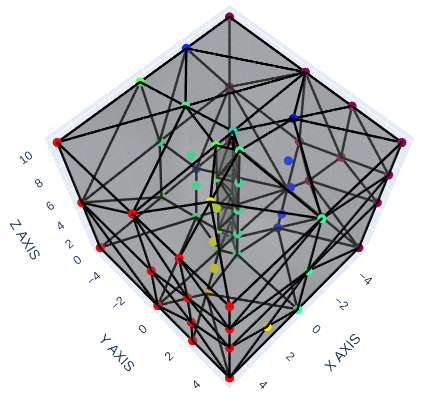
\includegraphics[width=1.75in]{Final Run, (cube - equilateral triangle hole 1 mm) meshpy plotly screenshot.png}\\ {\fontsize{10}{12}\selectfont Equilateral Triangle Hole, 1 mm}} & 
         \tstack{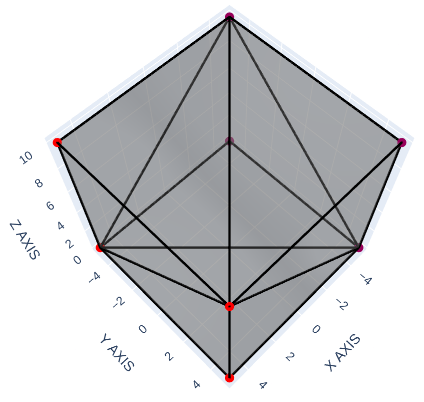
\includegraphics[width=1.75in]{Final Run, (cube - equilateral triangle hole 0 mm) meshpy plotly screenshot.png}\\ {\fontsize{10}{12}\selectfont Equilateral Triangle Hole, 0 mm}} \\
         \bottomrule
    \end{tabular}
    \end{center}
    \caption{MeshPy Plots displayed with Plotly of a cube with an equilateral triangle hole that decreases in size to the original shape.}
    \label{fig:cube_triangle_hole_meshpy_table}
\end{table}

\begin{table}[H]
\begin{center}
    \begin{tabular}{ccc}
         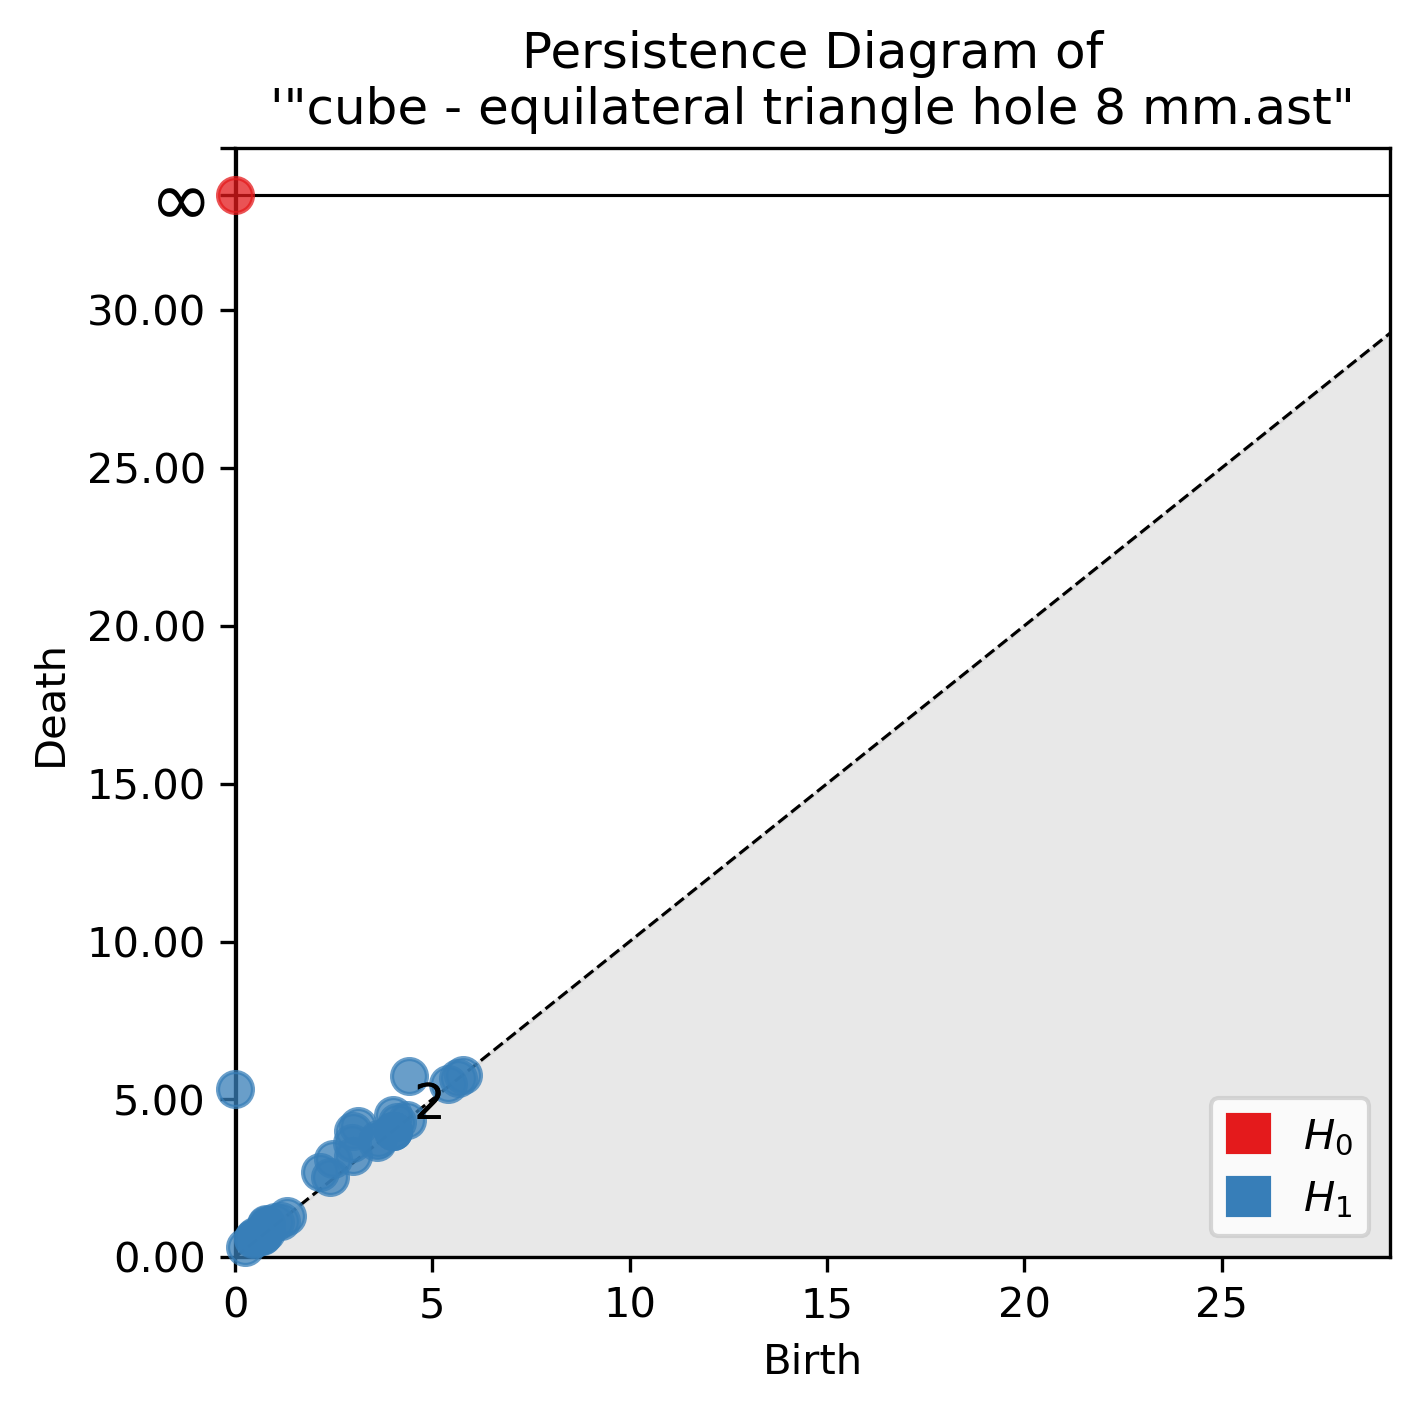
\includegraphics[width=1.875in]{Final Run, (cube - equilateral triangle hole 8 mm) persdia.png} &
         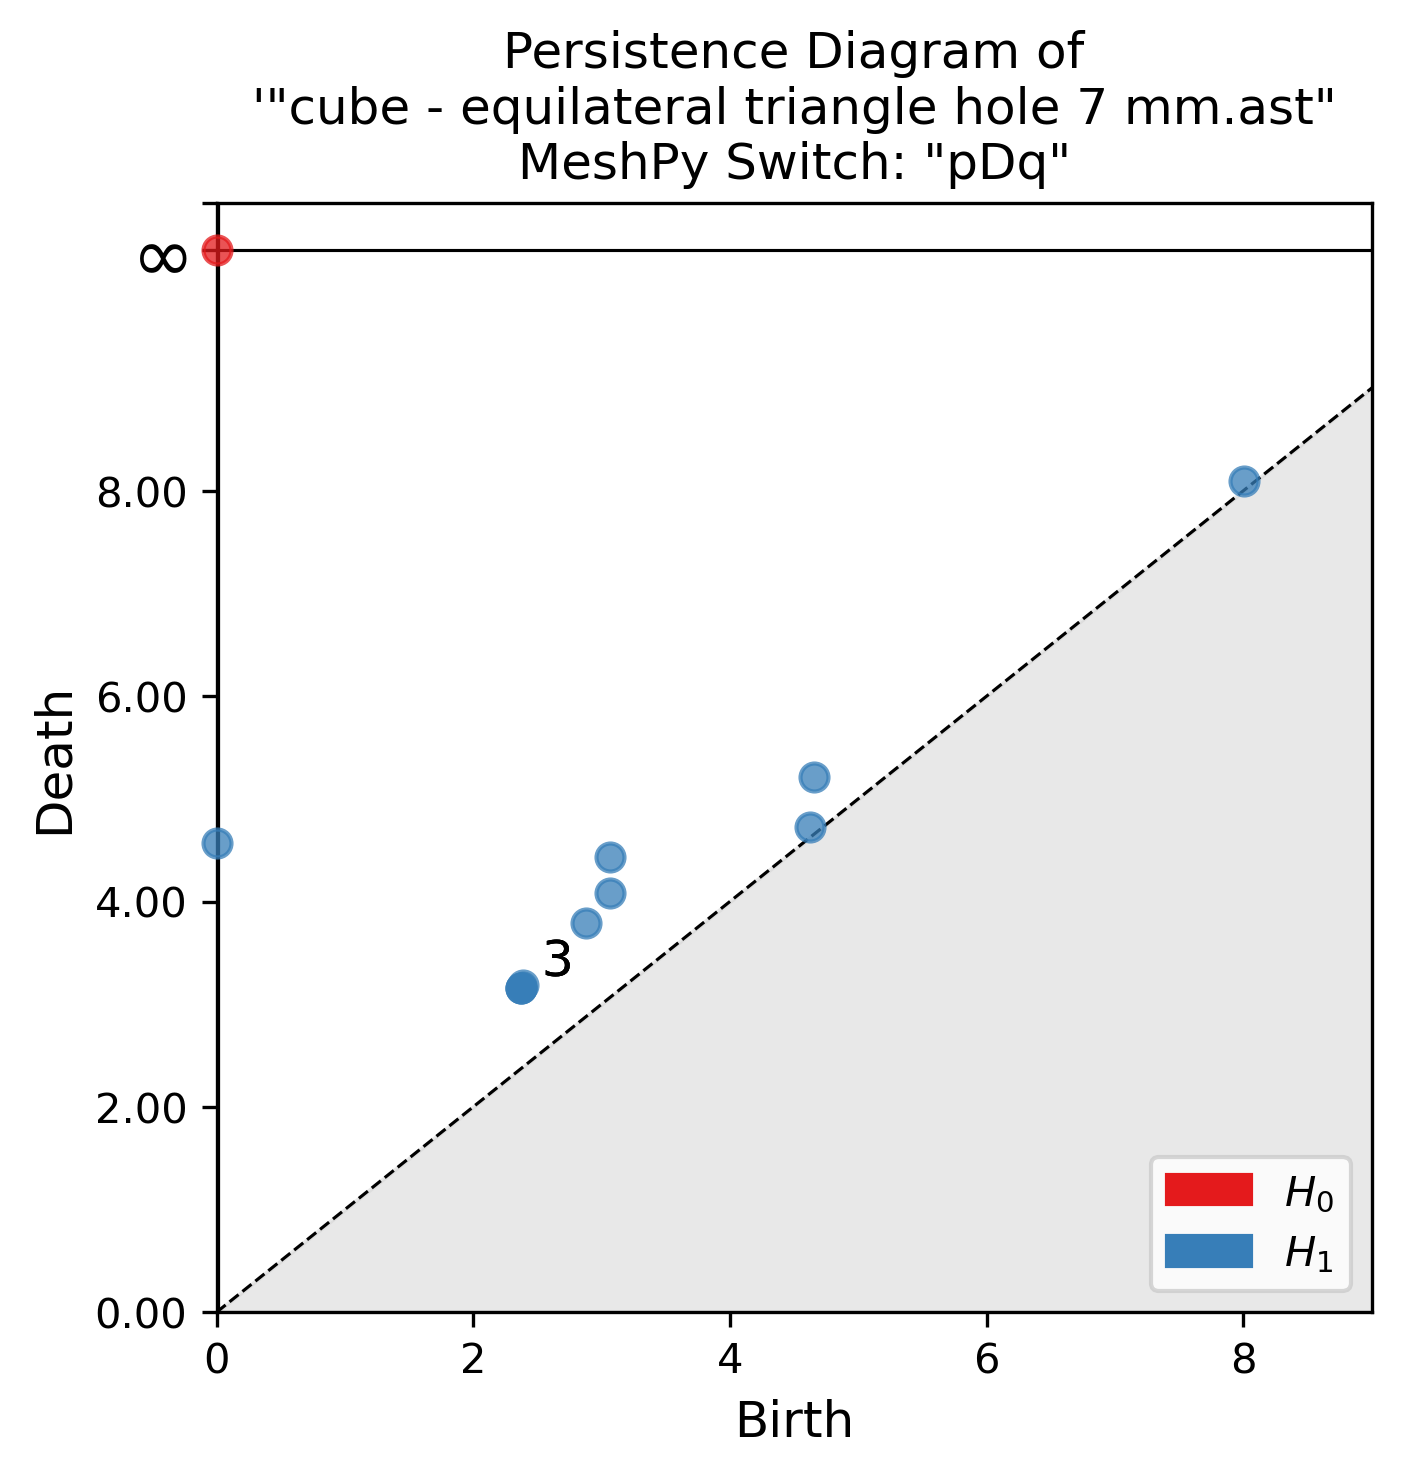
\includegraphics[width=1.875in]{Final Run, (cube - equilateral triangle hole 7 mm) persdia.png} &  
         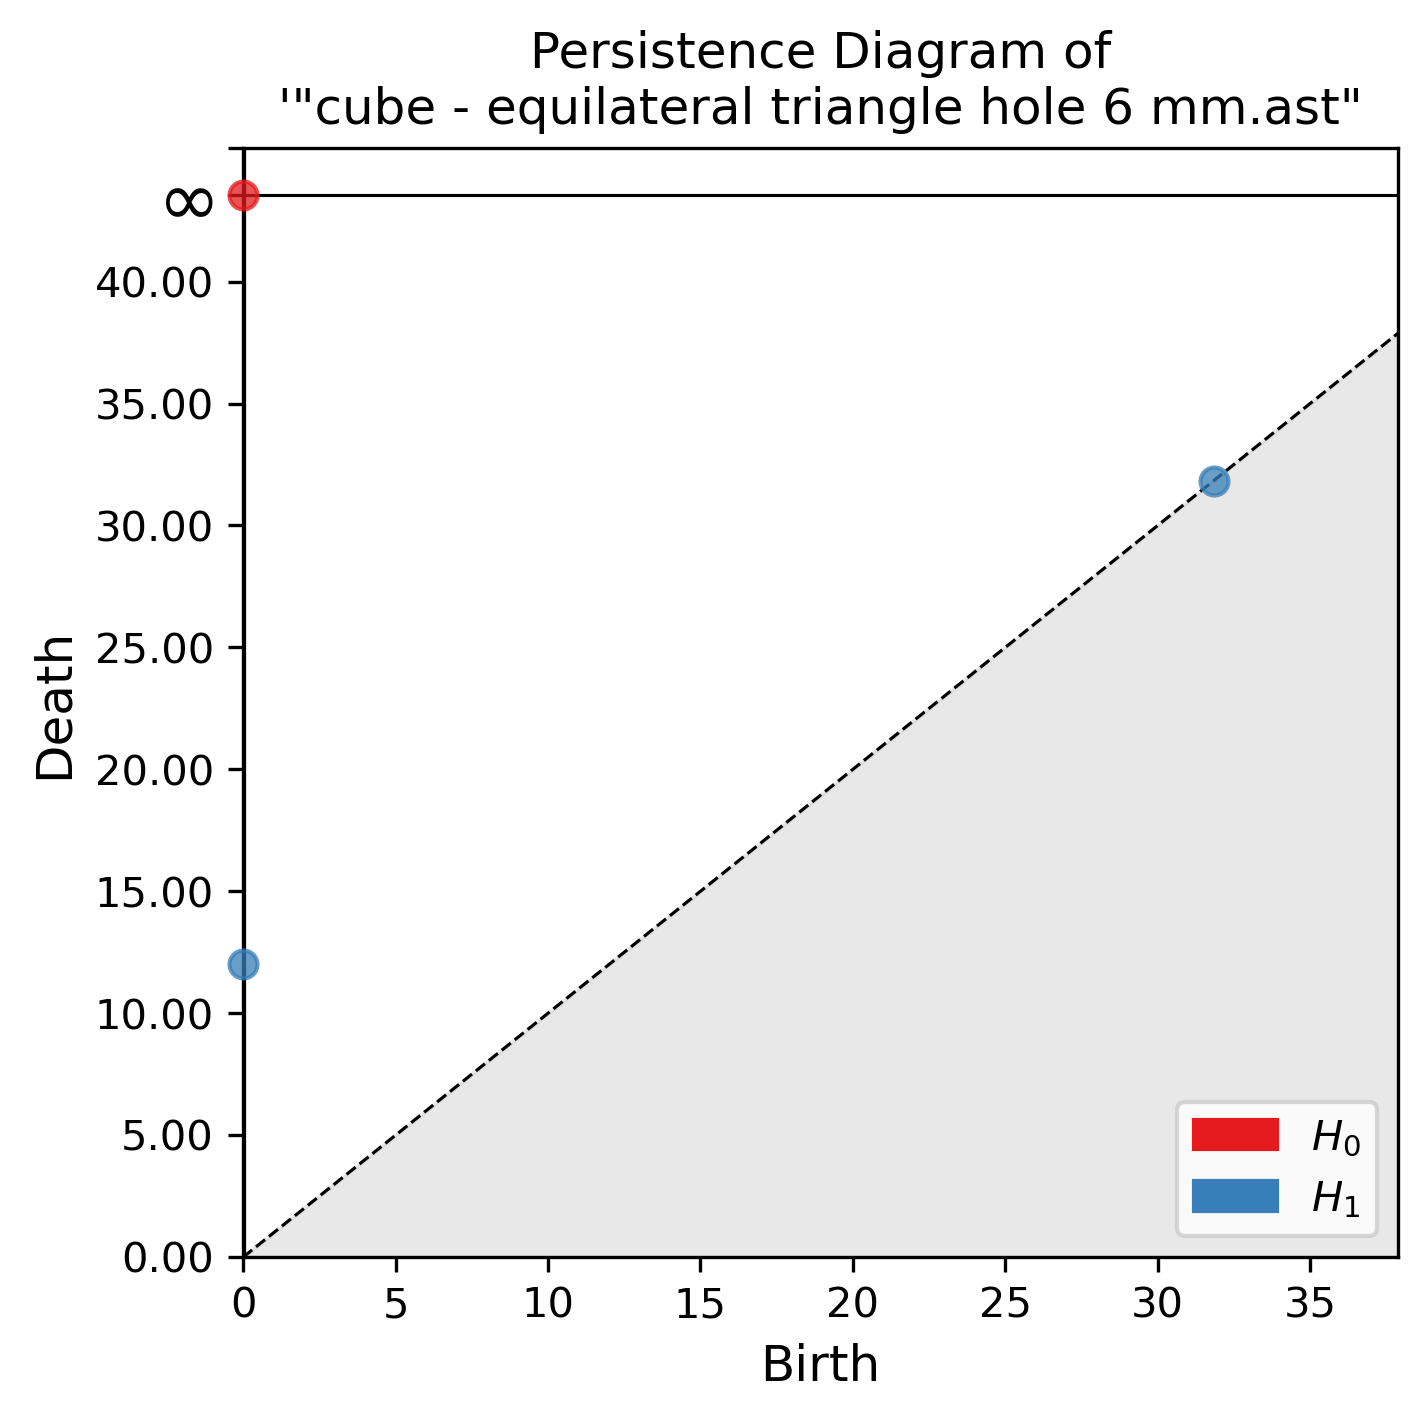
\includegraphics[width=1.875in]{Final Run, (cube - equilateral triangle hole 6 mm) persdia.png} \\
         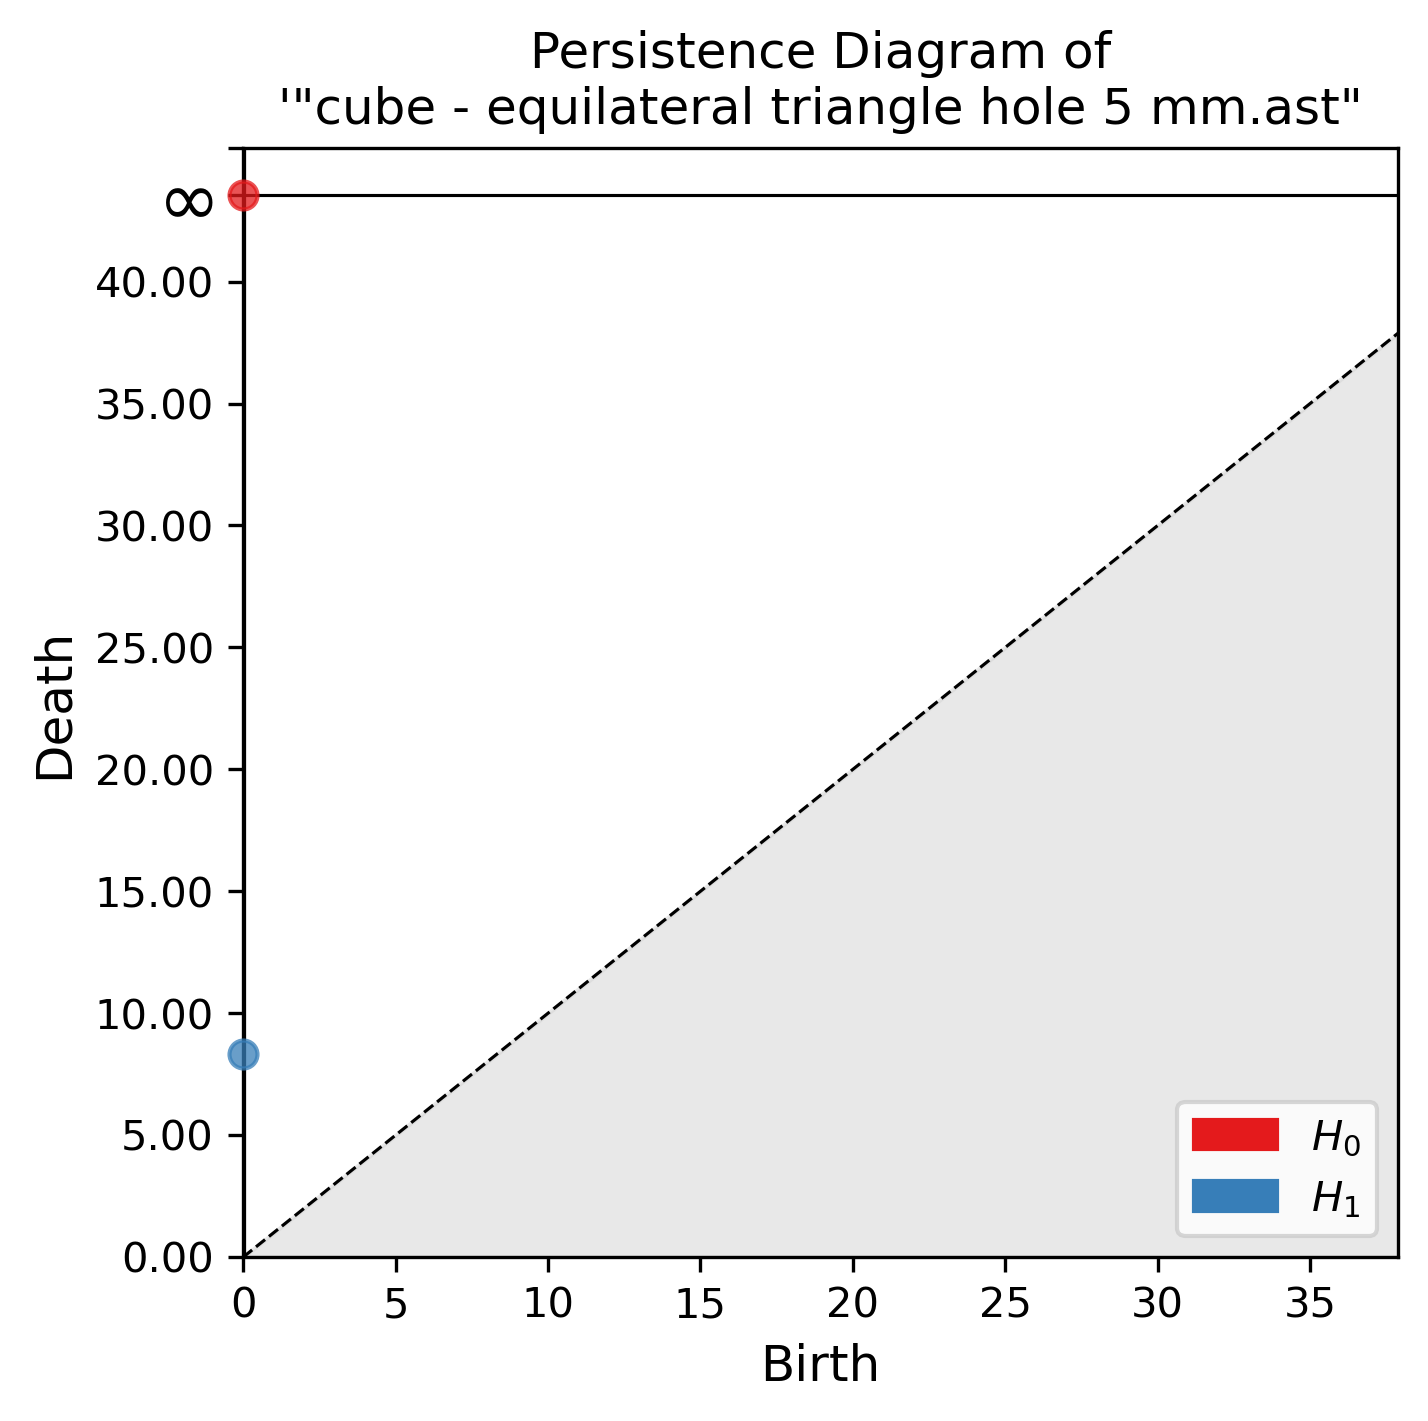
\includegraphics[width=1.875in]{Final Run, (cube - equilateral triangle hole 5 mm) persdia.png} & 
         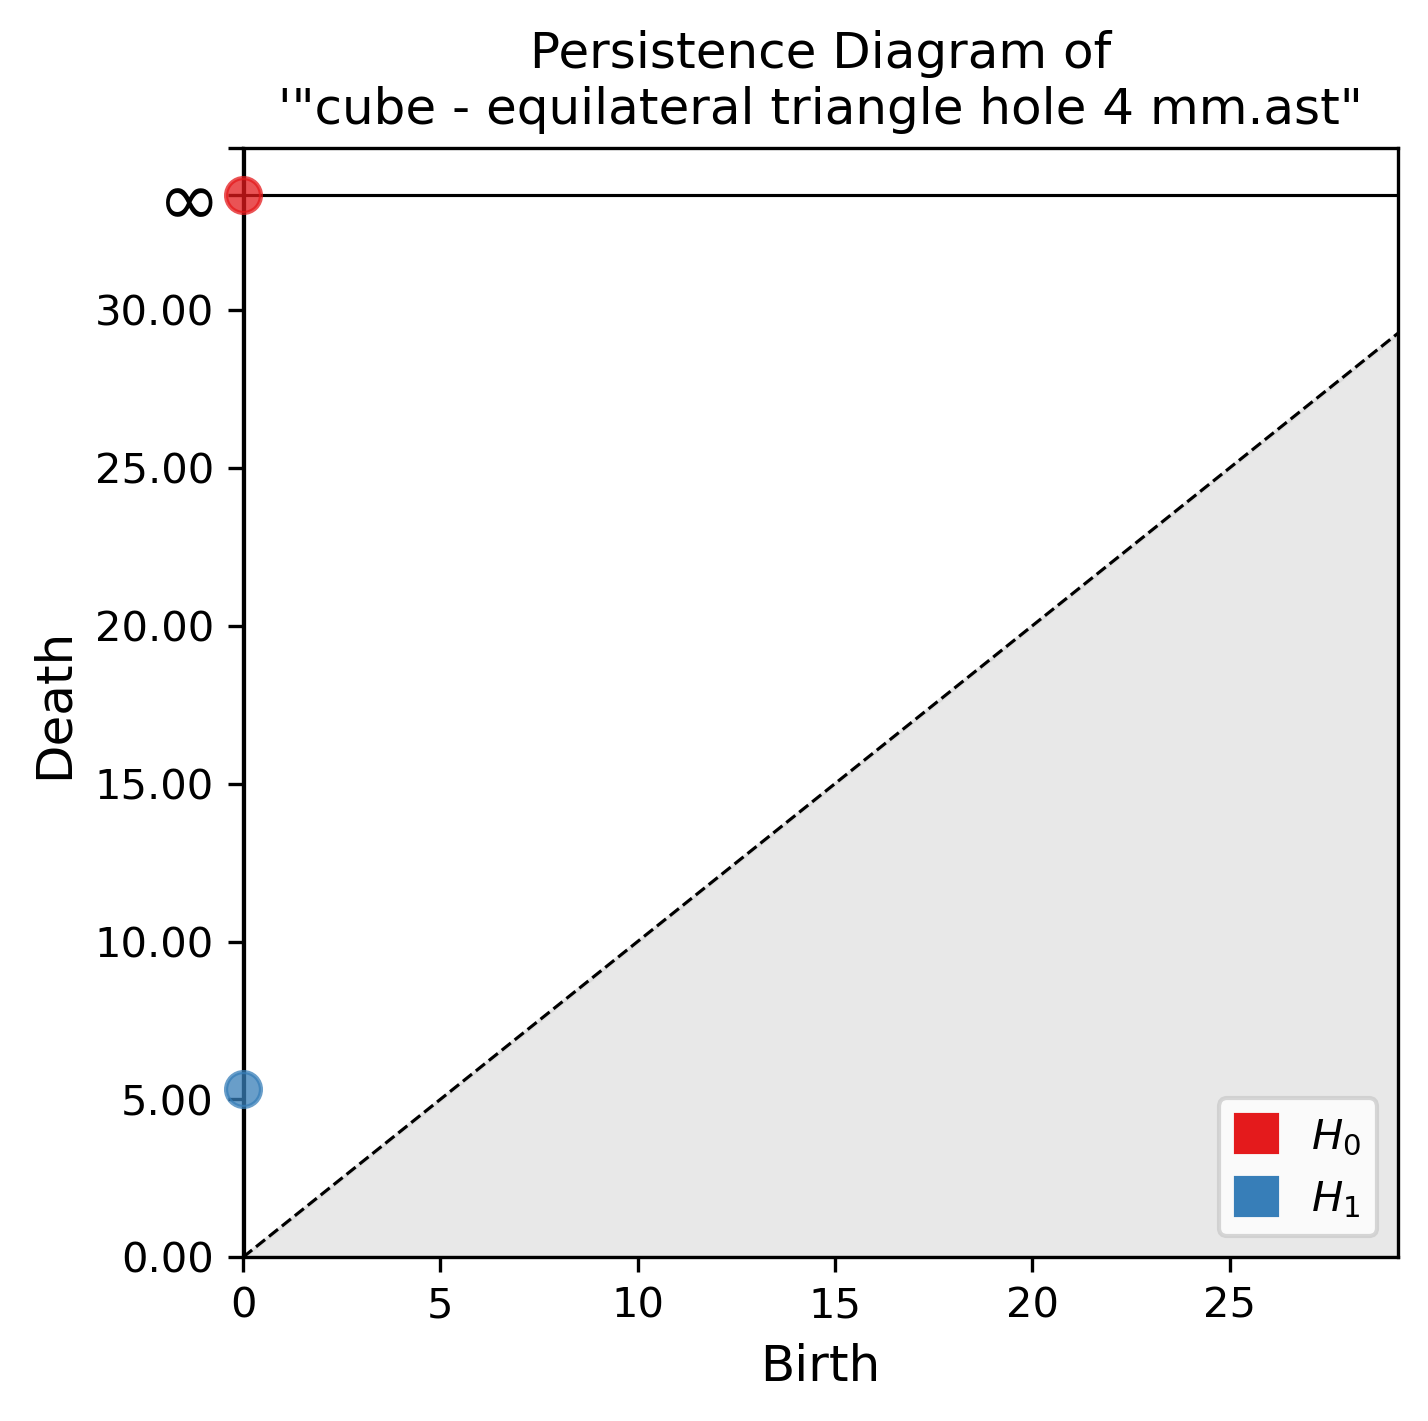
\includegraphics[width=1.875in]{Final Run, (cube - equilateral triangle hole 4 mm) persdia.png} & 
         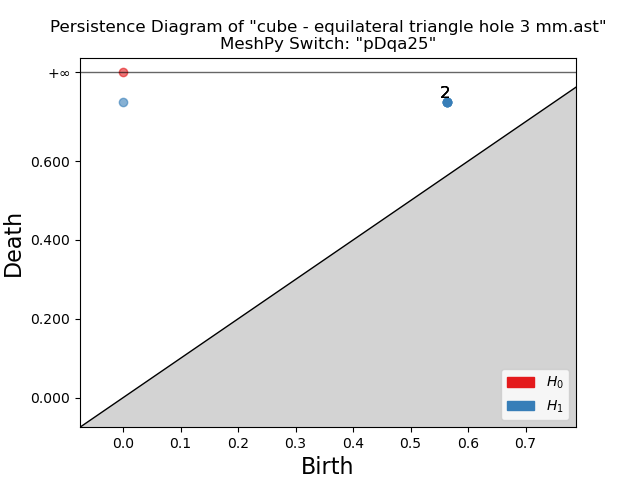
\includegraphics[width=1.875in]{Final Run, (cube - equilateral triangle hole 3 mm) persdia.png} \\
         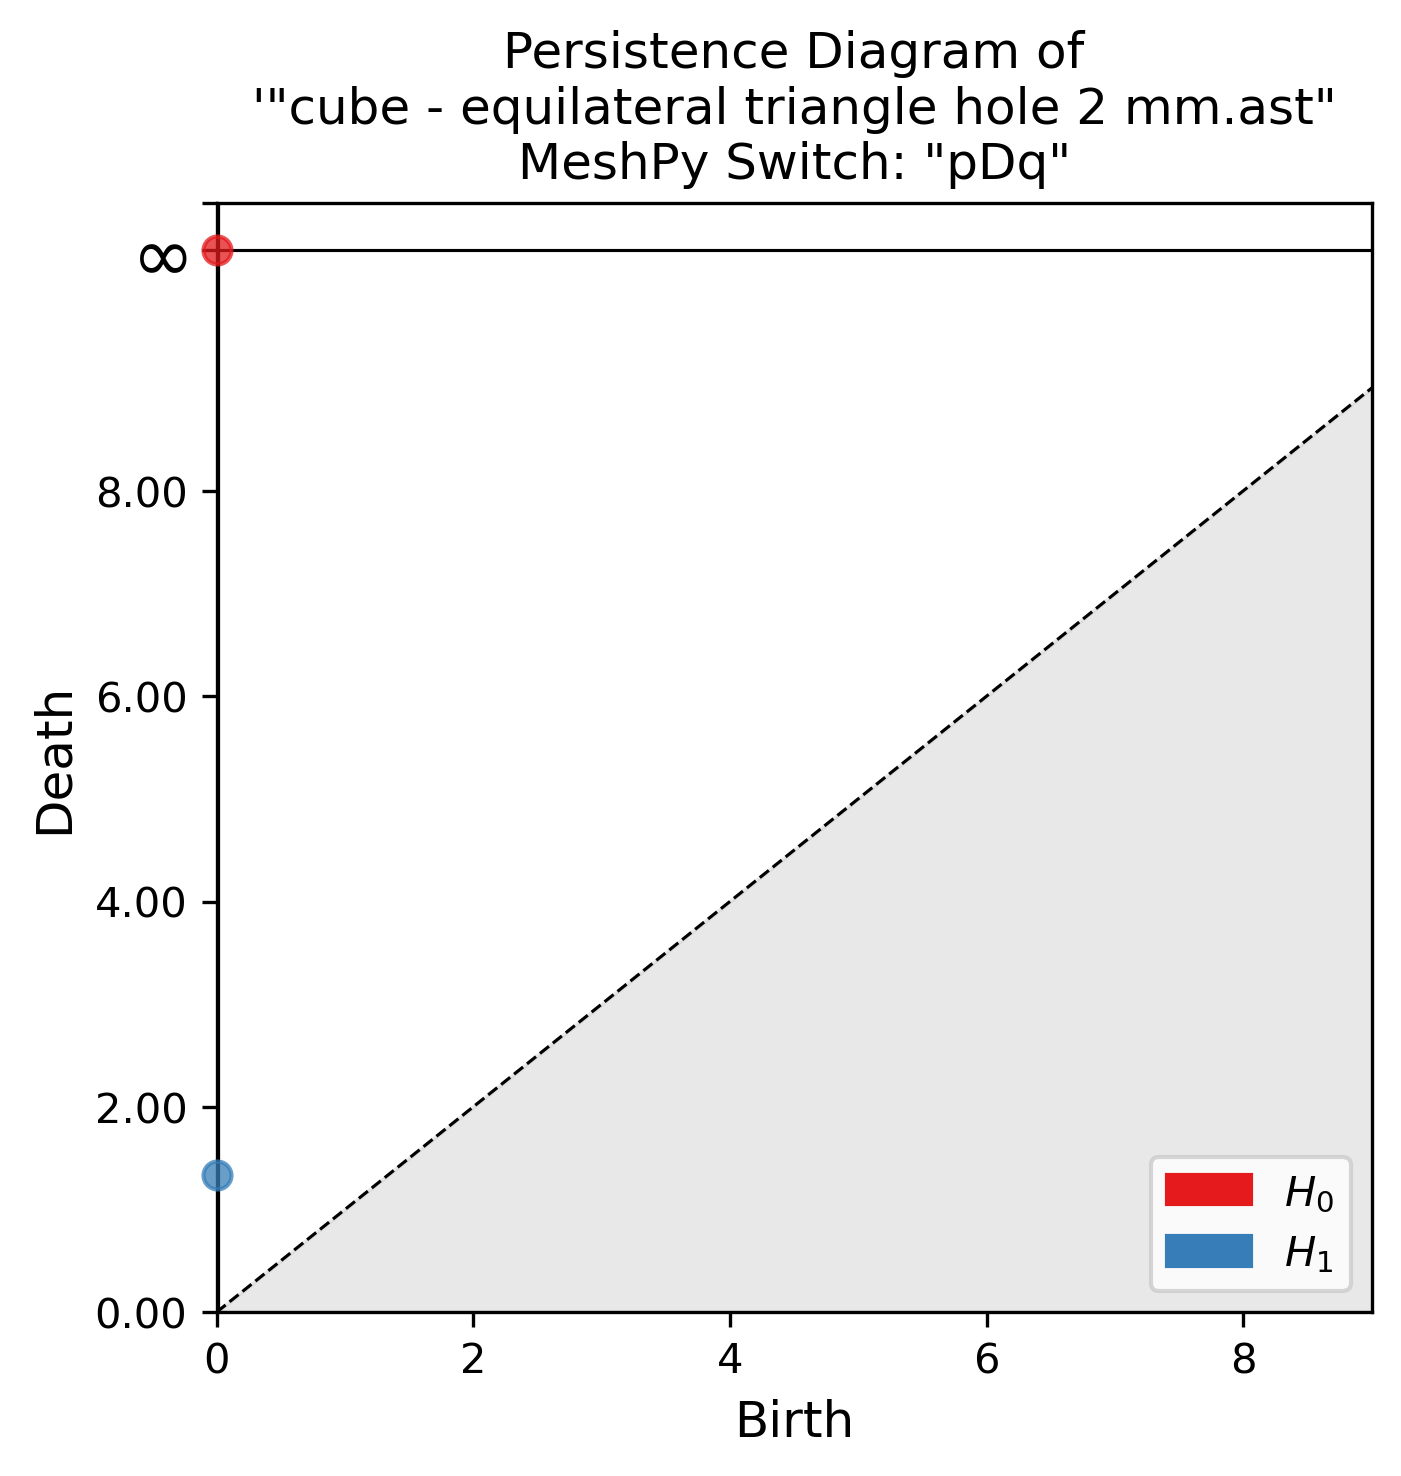
\includegraphics[width=1.875in]{Final Run, (cube - equilateral triangle hole 2 mm) persdia.png} & 
         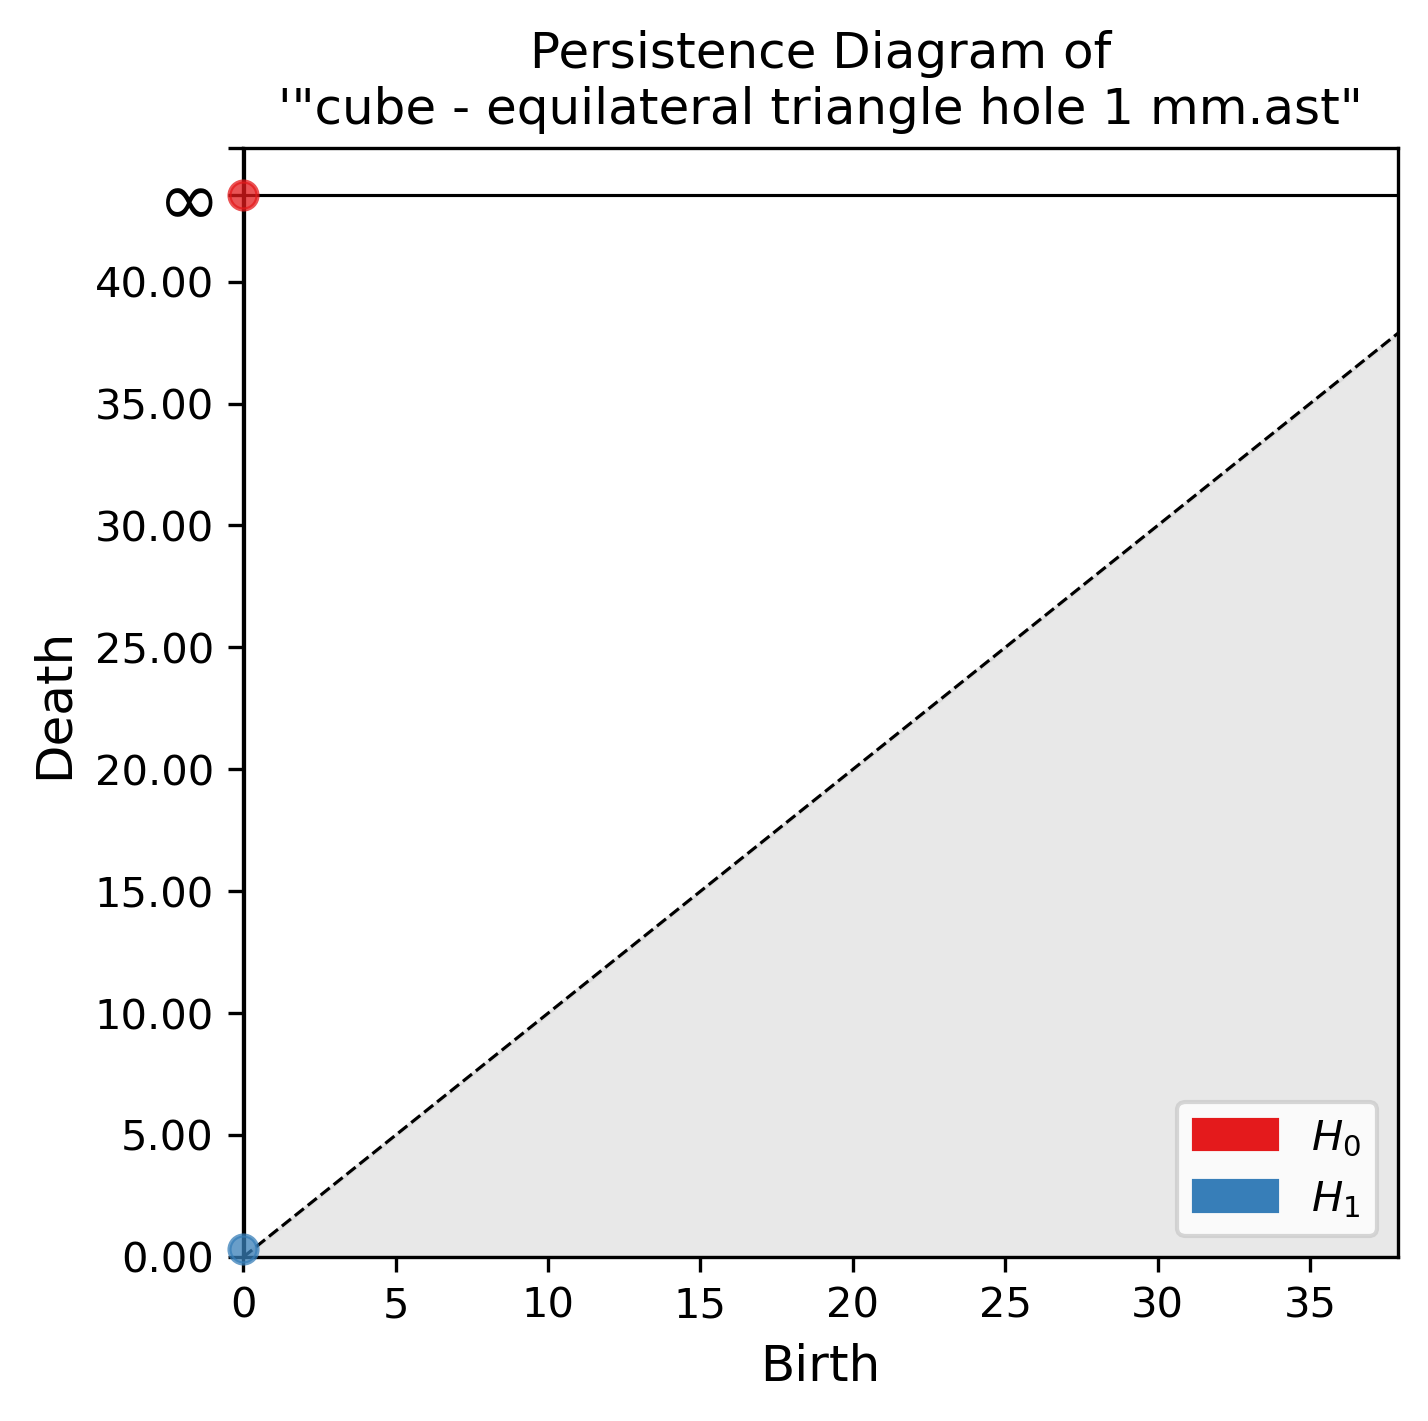
\includegraphics[width=1.875in]{Final Run, (cube - equilateral triangle hole 1 mm) persdia.png} & 
         \includegraphics[width=1.875in]{Final Run, (cube - equilateral triangle hole 0 mm) persdia.png} \\
    \end{tabular}
    \end{center}
    \caption{Persistence Diagrams of a cube with an equilateral triangle hole that decreases in size to the original shape.}
    \label{fig:cube_triangle_hole_persdia_table}
\end{table}

\newpage
\section{Rectangular Prism Ring with Cut}
A rectangular prism ring was created to model a solid torus with faster compute times from a more simple triangulation than a regular solid torus. The initial state has a 40mm cut which shrinks and dissapears.
\begin{table}[H]
\begin{center}
    \begin{tabular}{cccc}
    \toprule
         \tstack{\includegraphics[width=1.4in]{Final Run, (rect prism ring 40 mm cut) meshpy plotly screenshot.png}\\ {\fontsize{10}{12}\selectfont 40 mm cut}} &
         \tstack{\includegraphics[width=1.4in]{Final Run, (rect prism ring 35 mm cut) meshpy plotly screenshot.png}\\ {\fontsize{10}{12}\selectfont 35 mm cut}} &
         \tstack{\includegraphics[width=1.4in]{Final Run, (rect prism ring 30 mm cut) meshpy plotly screenshot.png}\\ {\fontsize{10}{12}\selectfont 30 mm cut}} &
         \tstack{\includegraphics[width=1.4in]{Final Run, (rect prism ring 25 mm cut) meshpy plotly screenshot.png}\\ {\fontsize{10}{12}\selectfont 25 mm cut}} \\ 
    \midrule
         \tstack{\includegraphics[width=1.4in]{Final Run, (rect prism ring 20 mm cut) meshpy plotly screenshot.png}\\ {\fontsize{10}{12}\selectfont 20 mm cut}} & 
         \tstack{\includegraphics[width=1.4in]{Final Run, (rect prism ring 15 mm cut) meshpy plotly screenshot.png}\\ {\fontsize{10}{12}\selectfont 15 mm cut}} &
         \tstack{\includegraphics[width=1.4in]{Final Run, (rect prism ring 10 mm cut) meshpy plotly screenshot.png}\\ {\fontsize{10}{12}\selectfont 10 mm cut}} & 
         \tstack{\includegraphics[width=1.4in]{Final Run, (rect prism ring 05 mm cut) meshpy plotly screenshot.png}\\ {\fontsize{10}{12}\selectfont 05 mm cut}} \\ 
    \midrule
         \tstack{\includegraphics[width=1.4in]{Final Run, (rect prism ring 03 mm cut) meshpy plotly screenshot.png}\\ {\fontsize{10}{12}\selectfont 03 mm cut}} &
         \tstack{\includegraphics[width=1.4in]{Final Run, (rect prism ring 02 mm cut) meshpy plotly screenshot.png}\\ {\fontsize{10}{12}\selectfont 02 mm cut}} &
         \tstack{\includegraphics[width=1.4in]{Final Run, (rect prism ring 01 mm cut) meshpy plotly screenshot.png}\\ {\fontsize{10}{12}\selectfont 01 mm cut}} &
         \tstack{\includegraphics[width=1.4in]{Final Run, (rect prism ring 00 mm cut) meshpy plotly screenshot.png}\\ {\fontsize{10}{12}\selectfont 00 mm cut}} \\
    \bottomrule
    \end{tabular}
    \end{center}
    \caption{MeshPy Plots displayed with Plotly of a rectangular prism ring with a cut that decreases to the original shape.}
    \label{fig:rect_prism_ring_meshpy_table}
\end{table}

\begin{table}[H]
\begin{center}
    \begin{tabular}{cccc}
         \includegraphics[width=0.24\textwidth]{Final Run, (rect prism ring 40 mm cut) persdia.png} &
         \includegraphics[width=0.24\textwidth]{Final Run, (rect prism ring 35 mm cut) persdia.png} &  
         \includegraphics[width=0.24\textwidth]{Final Run, (rect prism ring 30 mm cut) persdia.png} &
         \includegraphics[width=0.24\textwidth]{Final Run, (rect prism ring 25 mm cut) persdia.png} \\ 
         \includegraphics[width=0.24\textwidth]{Final Run, (rect prism ring 20 mm cut) persdia.png} & 
         \includegraphics[width=0.24\textwidth]{Final Run, (rect prism ring 15 mm cut) persdia.png} &
         \includegraphics[width=0.24\textwidth]{Final Run, (rect prism ring 10 mm cut) persdia.png} & 
         \includegraphics[width=0.24\textwidth]{Final Run, (rect prism ring 05 mm cut) persdia.png} \\ 
         \includegraphics[width=0.24\textwidth]{Final Run, (rect prism ring 03 mm cut) persdia.png} &
         \includegraphics[width=0.24\textwidth]{Final Run, (rect prism ring 02 mm cut) persdia.png} &
         \includegraphics[width=0.24\textwidth]{Final Run, (rect prism ring 01 mm cut) persdia.png} &
         \includegraphics[width=0.24\textwidth]{Final Run, (rect prism ring 00 mm cut) persdia.png} \\
    \end{tabular}
    \end{center}
    \caption{Persistence Diagrams of a rectangular prism ring with a cut that decreases to the original shape.}
    \label{fig:rect_prism_ring_persdia_table}
\end{table}

\subsection{Discussion}

\chapter{Conclusion}
\section{Future Work}
measure of topological stability - quantative measure
Do void things with better python code tetrahedralizing

\bibliography{thesis_bib}
\bibliographystyle{plain}
\backmatter
\end{document}
